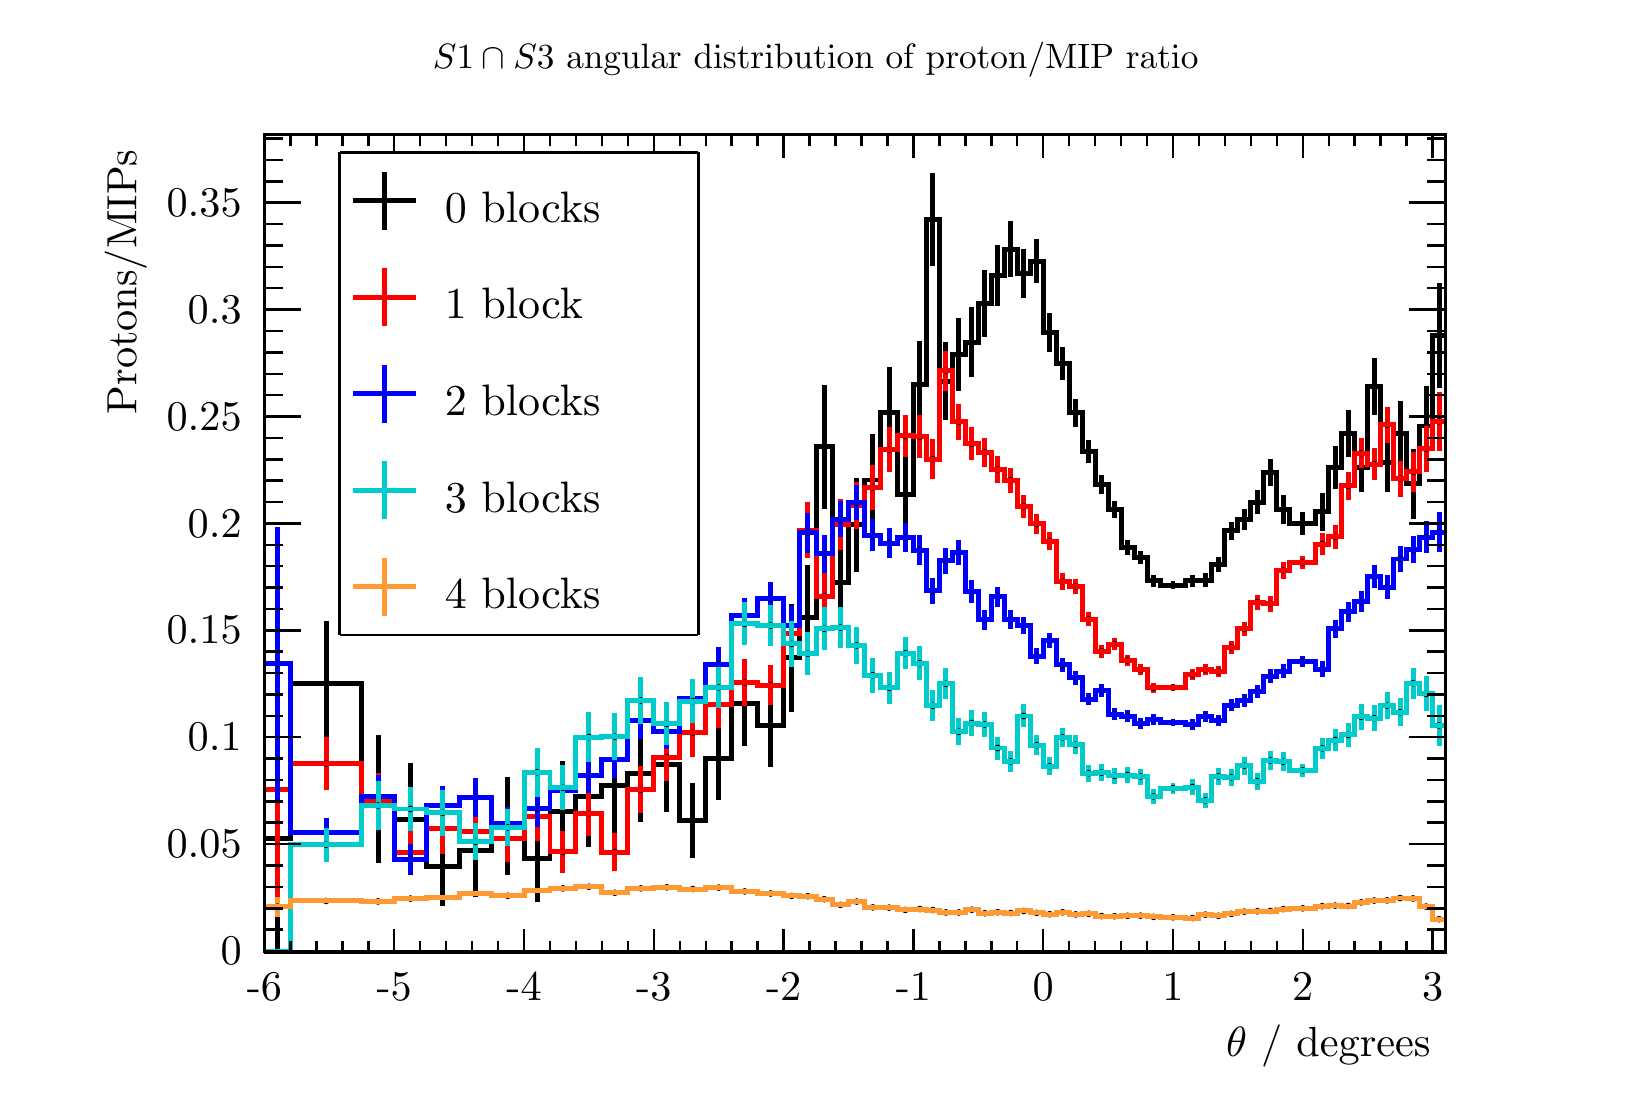
\begin{tikzpicture}
\pgfdeclareplotmark{cross} {
\pgfpathmoveto{\pgfpoint{-0.3\pgfplotmarksize}{\pgfplotmarksize}}
\pgfpathlineto{\pgfpoint{+0.3\pgfplotmarksize}{\pgfplotmarksize}}
\pgfpathlineto{\pgfpoint{+0.3\pgfplotmarksize}{0.3\pgfplotmarksize}}
\pgfpathlineto{\pgfpoint{+1\pgfplotmarksize}{0.3\pgfplotmarksize}}
\pgfpathlineto{\pgfpoint{+1\pgfplotmarksize}{-0.3\pgfplotmarksize}}
\pgfpathlineto{\pgfpoint{+0.3\pgfplotmarksize}{-0.3\pgfplotmarksize}}
\pgfpathlineto{\pgfpoint{+0.3\pgfplotmarksize}{-1.\pgfplotmarksize}}
\pgfpathlineto{\pgfpoint{-0.3\pgfplotmarksize}{-1.\pgfplotmarksize}}
\pgfpathlineto{\pgfpoint{-0.3\pgfplotmarksize}{-0.3\pgfplotmarksize}}
\pgfpathlineto{\pgfpoint{-1.\pgfplotmarksize}{-0.3\pgfplotmarksize}}
\pgfpathlineto{\pgfpoint{-1.\pgfplotmarksize}{0.3\pgfplotmarksize}}
\pgfpathlineto{\pgfpoint{-0.3\pgfplotmarksize}{0.3\pgfplotmarksize}}
\pgfpathclose
\pgfusepathqstroke
}
\pgfdeclareplotmark{cross*} {
\pgfpathmoveto{\pgfpoint{-0.3\pgfplotmarksize}{\pgfplotmarksize}}
\pgfpathlineto{\pgfpoint{+0.3\pgfplotmarksize}{\pgfplotmarksize}}
\pgfpathlineto{\pgfpoint{+0.3\pgfplotmarksize}{0.3\pgfplotmarksize}}
\pgfpathlineto{\pgfpoint{+1\pgfplotmarksize}{0.3\pgfplotmarksize}}
\pgfpathlineto{\pgfpoint{+1\pgfplotmarksize}{-0.3\pgfplotmarksize}}
\pgfpathlineto{\pgfpoint{+0.3\pgfplotmarksize}{-0.3\pgfplotmarksize}}
\pgfpathlineto{\pgfpoint{+0.3\pgfplotmarksize}{-1.\pgfplotmarksize}}
\pgfpathlineto{\pgfpoint{-0.3\pgfplotmarksize}{-1.\pgfplotmarksize}}
\pgfpathlineto{\pgfpoint{-0.3\pgfplotmarksize}{-0.3\pgfplotmarksize}}
\pgfpathlineto{\pgfpoint{-1.\pgfplotmarksize}{-0.3\pgfplotmarksize}}
\pgfpathlineto{\pgfpoint{-1.\pgfplotmarksize}{0.3\pgfplotmarksize}}
\pgfpathlineto{\pgfpoint{-0.3\pgfplotmarksize}{0.3\pgfplotmarksize}}
\pgfpathclose
\pgfusepathqfillstroke
}
\pgfdeclareplotmark{newstar} {
\pgfpathmoveto{\pgfqpoint{0pt}{\pgfplotmarksize}}
\pgfpathlineto{\pgfqpointpolar{44}{0.5\pgfplotmarksize}}
\pgfpathlineto{\pgfqpointpolar{18}{\pgfplotmarksize}}
\pgfpathlineto{\pgfqpointpolar{-20}{0.5\pgfplotmarksize}}
\pgfpathlineto{\pgfqpointpolar{-54}{\pgfplotmarksize}}
\pgfpathlineto{\pgfqpointpolar{-90}{0.5\pgfplotmarksize}}
\pgfpathlineto{\pgfqpointpolar{234}{\pgfplotmarksize}}
\pgfpathlineto{\pgfqpointpolar{198}{0.5\pgfplotmarksize}}
\pgfpathlineto{\pgfqpointpolar{162}{\pgfplotmarksize}}
\pgfpathlineto{\pgfqpointpolar{134}{0.5\pgfplotmarksize}}
\pgfpathclose
\pgfusepathqstroke
}
\pgfdeclareplotmark{newstar*} {
\pgfpathmoveto{\pgfqpoint{0pt}{\pgfplotmarksize}}
\pgfpathlineto{\pgfqpointpolar{44}{0.5\pgfplotmarksize}}
\pgfpathlineto{\pgfqpointpolar{18}{\pgfplotmarksize}}
\pgfpathlineto{\pgfqpointpolar{-20}{0.5\pgfplotmarksize}}
\pgfpathlineto{\pgfqpointpolar{-54}{\pgfplotmarksize}}
\pgfpathlineto{\pgfqpointpolar{-90}{0.5\pgfplotmarksize}}
\pgfpathlineto{\pgfqpointpolar{234}{\pgfplotmarksize}}
\pgfpathlineto{\pgfqpointpolar{198}{0.5\pgfplotmarksize}}
\pgfpathlineto{\pgfqpointpolar{162}{\pgfplotmarksize}}
\pgfpathlineto{\pgfqpointpolar{134}{0.5\pgfplotmarksize}}
\pgfpathclose
\pgfusepathqfillstroke
}
\definecolor{c}{rgb}{1,1,1};
\draw [color=c, fill=c] (0,0) rectangle (20,13.4957);
\draw [color=c, fill=c] (3,1.75444) rectangle (18,12.1461);
\definecolor{c}{rgb}{0,0,0};
\draw [c,line width=0.9] (3,1.75444) -- (3,12.1461) -- (18,12.1461) -- (18,1.75444) -- (3,1.75444);
\definecolor{c}{rgb}{1,1,1};
\draw [color=c, fill=c] (3,1.75444) rectangle (18,12.1461);
\definecolor{c}{rgb}{0,0,0};
\draw [c,line width=0.9] (3,1.75444) -- (3,12.1461) -- (18,12.1461) -- (18,1.75444) -- (3,1.75444);
\draw [c,line width=0.9] (3,1.77619) -- (3.32967,1.77619) -- (3.32967,1.77619) -- (4.23626,1.77619) -- (4.23626,1.77619) -- (4.64835,1.77619) -- (4.64835,1.77619) -- (5.06044,1.77619) -- (5.06044,1.77619) -- (5.47253,1.77619) -- (5.47253,1.77619) --
 (5.88462,1.77619) -- (5.88462,1.77619) -- (6.2967,1.77619) -- (6.2967,1.77619) -- (6.62637,1.77619) -- (6.62637,1.77619) -- (6.95604,1.77619) -- (6.95604,1.77619) -- (7.28571,1.77619) -- (7.28571,1.77619) -- (7.61538,1.77619) -- (7.61538,1.77619) --
 (7.94506,1.77619) -- (7.94506,1.77619) -- (8.27472,1.77619) -- (8.27472,1.77619) -- (8.6044,1.77619) -- (8.6044,1.77619) -- (8.93407,1.77619) -- (8.93407,1.77619) -- (9.26374,1.77619) -- (9.26374,1.77619) -- (9.59341,1.77619) -- (9.59341,1.77619) --
 (9.79945,1.77619) -- (9.79945,1.77619) -- (10.0055,1.77619) -- (10.0055,1.77619) -- (10.2115,1.77619) -- (10.2115,1.77619) -- (10.4176,1.77619) -- (10.4176,1.77619) -- (10.6236,1.77619) -- (10.6236,1.77619) -- (10.8297,1.77619) -- (10.8297,1.77619)
 -- (11.0357,1.77619) -- (11.0357,1.77619) -- (11.2418,1.77619) -- (11.2418,1.77619) -- (11.4066,1.77619) -- (11.4066,1.77619) -- (11.5714,1.77619) -- (11.5714,1.77619) -- (11.7363,1.77619) -- (11.7363,1.77619) -- (11.9011,1.77619) --
 (11.9011,1.77619) -- (12.0659,1.77619) -- (12.0659,1.77619) -- (12.2308,1.77619) -- (12.2308,1.77619) -- (12.3956,1.77619) -- (12.3956,1.77619) -- (12.5604,1.77619) -- (12.5604,1.77619) -- (12.7253,1.77619) -- (12.7253,1.77619) -- (12.8901,1.77619)
 -- (12.8901,1.77619) -- (13.0549,1.77619) -- (13.0549,1.77619) -- (13.2198,1.77619) -- (13.2198,1.77619) -- (13.3846,1.77619) -- (13.3846,1.77619) -- (13.5495,1.77619) -- (13.5495,1.77619) -- (13.7143,1.77619) -- (13.7143,1.77619) --
 (13.8791,1.77619) -- (13.8791,1.77619) -- (14.044,1.77619) -- (14.044,1.77619) -- (14.2088,1.77619) -- (14.2088,1.77619) -- (14.3736,1.77619) -- (14.3736,1.77619) -- (14.7033,1.77619) -- (14.7033,1.77619) -- (14.8681,1.77619) -- (14.8681,1.77619) --
 (15.033,1.77619) -- (15.033,1.77619) -- (15.1978,1.77619) -- (15.1978,1.77619) -- (15.3626,1.77619) -- (15.3626,1.77619) -- (15.5275,1.77619) -- (15.5275,1.77619) -- (15.6923,1.77619) -- (15.6923,1.77619) -- (15.8571,1.77619) -- (15.8571,1.77619) --
 (16.022,1.77619) -- (16.022,1.77619) -- (16.3516,1.77619) -- (16.3516,1.77619) -- (16.5165,1.77619) -- (16.5165,1.77619) -- (16.6813,1.77619) -- (16.6813,1.77619) -- (16.8462,1.77619) -- (16.8462,1.77619) -- (17.011,1.77619) -- (17.011,1.77619) --
 (17.1758,1.77619) -- (17.1758,1.77619) -- (17.3407,1.77619) -- (17.3407,1.77619) -- (17.5055,1.77619) -- (17.5055,1.77619) -- (17.6703,1.77619) -- (17.6703,1.77619) -- (17.8352,1.77619) -- (17.8352,1.77619) -- (18,1.77619);
\draw [c,line width=0.9] (3,1.75444) -- (18,1.75444);
\draw [c,line width=0.9] (3,2.05809) -- (3,1.75444);
\draw [c,line width=0.9] (3.32967,1.90627) -- (3.32967,1.75444);
\draw [c,line width=0.9] (3.65934,1.90627) -- (3.65934,1.75444);
\draw [c,line width=0.9] (3.98901,1.90627) -- (3.98901,1.75444);
\draw [c,line width=0.9] (4.31868,1.90627) -- (4.31868,1.75444);
\draw [c,line width=0.9] (4.64835,2.05809) -- (4.64835,1.75444);
\draw [c,line width=0.9] (4.97802,1.90627) -- (4.97802,1.75444);
\draw [c,line width=0.9] (5.30769,1.90627) -- (5.30769,1.75444);
\draw [c,line width=0.9] (5.63736,1.90627) -- (5.63736,1.75444);
\draw [c,line width=0.9] (5.96703,1.90627) -- (5.96703,1.75444);
\draw [c,line width=0.9] (6.2967,2.05809) -- (6.2967,1.75444);
\draw [c,line width=0.9] (6.62637,1.90627) -- (6.62637,1.75444);
\draw [c,line width=0.9] (6.95604,1.90627) -- (6.95604,1.75444);
\draw [c,line width=0.9] (7.28571,1.90627) -- (7.28571,1.75444);
\draw [c,line width=0.9] (7.61538,1.90627) -- (7.61538,1.75444);
\draw [c,line width=0.9] (7.94506,2.05809) -- (7.94506,1.75444);
\draw [c,line width=0.9] (8.27472,1.90627) -- (8.27472,1.75444);
\draw [c,line width=0.9] (8.6044,1.90627) -- (8.6044,1.75444);
\draw [c,line width=0.9] (8.93407,1.90627) -- (8.93407,1.75444);
\draw [c,line width=0.9] (9.26374,1.90627) -- (9.26374,1.75444);
\draw [c,line width=0.9] (9.59341,2.05809) -- (9.59341,1.75444);
\draw [c,line width=0.9] (9.92308,1.90627) -- (9.92308,1.75444);
\draw [c,line width=0.9] (10.2527,1.90627) -- (10.2527,1.75444);
\draw [c,line width=0.9] (10.5824,1.90627) -- (10.5824,1.75444);
\draw [c,line width=0.9] (10.9121,1.90627) -- (10.9121,1.75444);
\draw [c,line width=0.9] (11.2418,2.05809) -- (11.2418,1.75444);
\draw [c,line width=0.9] (11.5714,1.90627) -- (11.5714,1.75444);
\draw [c,line width=0.9] (11.9011,1.90627) -- (11.9011,1.75444);
\draw [c,line width=0.9] (12.2308,1.90627) -- (12.2308,1.75444);
\draw [c,line width=0.9] (12.5604,1.90627) -- (12.5604,1.75444);
\draw [c,line width=0.9] (12.8901,2.05809) -- (12.8901,1.75444);
\draw [c,line width=0.9] (13.2198,1.90627) -- (13.2198,1.75444);
\draw [c,line width=0.9] (13.5495,1.90627) -- (13.5495,1.75444);
\draw [c,line width=0.9] (13.8791,1.90627) -- (13.8791,1.75444);
\draw [c,line width=0.9] (14.2088,1.90627) -- (14.2088,1.75444);
\draw [c,line width=0.9] (14.5385,2.05809) -- (14.5385,1.75444);
\draw [c,line width=0.9] (14.8681,1.90627) -- (14.8681,1.75444);
\draw [c,line width=0.9] (15.1978,1.90627) -- (15.1978,1.75444);
\draw [c,line width=0.9] (15.5275,1.90627) -- (15.5275,1.75444);
\draw [c,line width=0.9] (15.8571,1.90627) -- (15.8571,1.75444);
\draw [c,line width=0.9] (16.1868,2.05809) -- (16.1868,1.75444);
\draw [c,line width=0.9] (16.5165,1.90627) -- (16.5165,1.75444);
\draw [c,line width=0.9] (16.8462,1.90627) -- (16.8462,1.75444);
\draw [c,line width=0.9] (17.1758,1.90627) -- (17.1758,1.75444);
\draw [c,line width=0.9] (17.5055,1.90627) -- (17.5055,1.75444);
\draw [c,line width=0.9] (17.8352,2.05809) -- (17.8352,1.75444);
\draw [c,line width=0.9] (17.8352,2.05809) -- (17.8352,1.75444);
\draw [anchor=base] (3,1.14713) node[scale=1.52731, color=c, rotate=0]{-6};
\draw [anchor=base] (4.64835,1.14713) node[scale=1.52731, color=c, rotate=0]{-5};
\draw [anchor=base] (6.2967,1.14713) node[scale=1.52731, color=c, rotate=0]{-4};
\draw [anchor=base] (7.94506,1.14713) node[scale=1.52731, color=c, rotate=0]{-3};
\draw [anchor=base] (9.59341,1.14713) node[scale=1.52731, color=c, rotate=0]{-2};
\draw [anchor=base] (11.2418,1.14713) node[scale=1.52731, color=c, rotate=0]{-1};
\draw [anchor=base] (12.8901,1.14713) node[scale=1.52731, color=c, rotate=0]{0};
\draw [anchor=base] (14.5385,1.14713) node[scale=1.52731, color=c, rotate=0]{1};
\draw [anchor=base] (16.1868,1.14713) node[scale=1.52731, color=c, rotate=0]{2};
\draw [anchor=base] (17.8352,1.14713) node[scale=1.52731, color=c, rotate=0]{3};
\draw [anchor= east] (18,0.566819) node[scale=1.52731, color=c, rotate=0]{$ \theta$ / degrees};
\draw [c,line width=0.9] (3,12.1461) -- (18,12.1461);
\draw [c,line width=0.9] (3,11.8425) -- (3,12.1461);
\draw [c,line width=0.9] (3.32967,11.9943) -- (3.32967,12.1461);
\draw [c,line width=0.9] (3.65934,11.9943) -- (3.65934,12.1461);
\draw [c,line width=0.9] (3.98901,11.9943) -- (3.98901,12.1461);
\draw [c,line width=0.9] (4.31868,11.9943) -- (4.31868,12.1461);
\draw [c,line width=0.9] (4.64835,11.8425) -- (4.64835,12.1461);
\draw [c,line width=0.9] (4.97802,11.9943) -- (4.97802,12.1461);
\draw [c,line width=0.9] (5.30769,11.9943) -- (5.30769,12.1461);
\draw [c,line width=0.9] (5.63736,11.9943) -- (5.63736,12.1461);
\draw [c,line width=0.9] (5.96703,11.9943) -- (5.96703,12.1461);
\draw [c,line width=0.9] (6.2967,11.8425) -- (6.2967,12.1461);
\draw [c,line width=0.9] (6.62637,11.9943) -- (6.62637,12.1461);
\draw [c,line width=0.9] (6.95604,11.9943) -- (6.95604,12.1461);
\draw [c,line width=0.9] (7.28571,11.9943) -- (7.28571,12.1461);
\draw [c,line width=0.9] (7.61538,11.9943) -- (7.61538,12.1461);
\draw [c,line width=0.9] (7.94506,11.8425) -- (7.94506,12.1461);
\draw [c,line width=0.9] (8.27472,11.9943) -- (8.27472,12.1461);
\draw [c,line width=0.9] (8.6044,11.9943) -- (8.6044,12.1461);
\draw [c,line width=0.9] (8.93407,11.9943) -- (8.93407,12.1461);
\draw [c,line width=0.9] (9.26374,11.9943) -- (9.26374,12.1461);
\draw [c,line width=0.9] (9.59341,11.8425) -- (9.59341,12.1461);
\draw [c,line width=0.9] (9.92308,11.9943) -- (9.92308,12.1461);
\draw [c,line width=0.9] (10.2527,11.9943) -- (10.2527,12.1461);
\draw [c,line width=0.9] (10.5824,11.9943) -- (10.5824,12.1461);
\draw [c,line width=0.9] (10.9121,11.9943) -- (10.9121,12.1461);
\draw [c,line width=0.9] (11.2418,11.8425) -- (11.2418,12.1461);
\draw [c,line width=0.9] (11.5714,11.9943) -- (11.5714,12.1461);
\draw [c,line width=0.9] (11.9011,11.9943) -- (11.9011,12.1461);
\draw [c,line width=0.9] (12.2308,11.9943) -- (12.2308,12.1461);
\draw [c,line width=0.9] (12.5604,11.9943) -- (12.5604,12.1461);
\draw [c,line width=0.9] (12.8901,11.8425) -- (12.8901,12.1461);
\draw [c,line width=0.9] (13.2198,11.9943) -- (13.2198,12.1461);
\draw [c,line width=0.9] (13.5495,11.9943) -- (13.5495,12.1461);
\draw [c,line width=0.9] (13.8791,11.9943) -- (13.8791,12.1461);
\draw [c,line width=0.9] (14.2088,11.9943) -- (14.2088,12.1461);
\draw [c,line width=0.9] (14.5385,11.8425) -- (14.5385,12.1461);
\draw [c,line width=0.9] (14.8681,11.9943) -- (14.8681,12.1461);
\draw [c,line width=0.9] (15.1978,11.9943) -- (15.1978,12.1461);
\draw [c,line width=0.9] (15.5275,11.9943) -- (15.5275,12.1461);
\draw [c,line width=0.9] (15.8571,11.9943) -- (15.8571,12.1461);
\draw [c,line width=0.9] (16.1868,11.8425) -- (16.1868,12.1461);
\draw [c,line width=0.9] (16.5165,11.9943) -- (16.5165,12.1461);
\draw [c,line width=0.9] (16.8462,11.9943) -- (16.8462,12.1461);
\draw [c,line width=0.9] (17.1758,11.9943) -- (17.1758,12.1461);
\draw [c,line width=0.9] (17.5055,11.9943) -- (17.5055,12.1461);
\draw [c,line width=0.9] (17.8352,11.8425) -- (17.8352,12.1461);
\draw [c,line width=0.9] (17.8352,11.8425) -- (17.8352,12.1461);
\draw [c,line width=0.9] (3,1.75444) -- (3,12.1461);
\draw [c,line width=0.9] (3.462,1.77619) -- (3,1.77619);
\draw [c,line width=0.9] (3.231,2.04772) -- (3,2.04772);
\draw [c,line width=0.9] (3.231,2.31924) -- (3,2.31924);
\draw [c,line width=0.9] (3.231,2.59077) -- (3,2.59077);
\draw [c,line width=0.9] (3.231,2.8623) -- (3,2.8623);
\draw [c,line width=0.9] (3.462,3.13382) -- (3,3.13382);
\draw [c,line width=0.9] (3.231,3.40535) -- (3,3.40535);
\draw [c,line width=0.9] (3.231,3.67687) -- (3,3.67687);
\draw [c,line width=0.9] (3.231,3.9484) -- (3,3.9484);
\draw [c,line width=0.9] (3.231,4.21993) -- (3,4.21993);
\draw [c,line width=0.9] (3.462,4.49145) -- (3,4.49145);
\draw [c,line width=0.9] (3.231,4.76298) -- (3,4.76298);
\draw [c,line width=0.9] (3.231,5.03451) -- (3,5.03451);
\draw [c,line width=0.9] (3.231,5.30603) -- (3,5.30603);
\draw [c,line width=0.9] (3.231,5.57756) -- (3,5.57756);
\draw [c,line width=0.9] (3.462,5.84908) -- (3,5.84908);
\draw [c,line width=0.9] (3.231,6.12061) -- (3,6.12061);
\draw [c,line width=0.9] (3.231,6.39214) -- (3,6.39214);
\draw [c,line width=0.9] (3.231,6.66366) -- (3,6.66366);
\draw [c,line width=0.9] (3.231,6.93519) -- (3,6.93519);
\draw [c,line width=0.9] (3.462,7.20672) -- (3,7.20672);
\draw [c,line width=0.9] (3.231,7.47824) -- (3,7.47824);
\draw [c,line width=0.9] (3.231,7.74977) -- (3,7.74977);
\draw [c,line width=0.9] (3.231,8.0213) -- (3,8.0213);
\draw [c,line width=0.9] (3.231,8.29282) -- (3,8.29282);
\draw [c,line width=0.9] (3.462,8.56435) -- (3,8.56435);
\draw [c,line width=0.9] (3.231,8.83587) -- (3,8.83587);
\draw [c,line width=0.9] (3.231,9.1074) -- (3,9.1074);
\draw [c,line width=0.9] (3.231,9.37893) -- (3,9.37893);
\draw [c,line width=0.9] (3.231,9.65045) -- (3,9.65045);
\draw [c,line width=0.9] (3.462,9.92198) -- (3,9.92198);
\draw [c,line width=0.9] (3.231,10.1935) -- (3,10.1935);
\draw [c,line width=0.9] (3.231,10.465) -- (3,10.465);
\draw [c,line width=0.9] (3.231,10.7366) -- (3,10.7366);
\draw [c,line width=0.9] (3.231,11.0081) -- (3,11.0081);
\draw [c,line width=0.9] (3.462,11.2796) -- (3,11.2796);
\draw [c,line width=0.9] (3.462,1.77619) -- (3,1.77619);
\draw [c,line width=0.9] (3.462,11.2796) -- (3,11.2796);
\draw [c,line width=0.9] (3.231,11.5511) -- (3,11.5511);
\draw [c,line width=0.9] (3.231,11.8227) -- (3,11.8227);
\draw [c,line width=0.9] (3.231,12.0942) -- (3,12.0942);
\draw [anchor= east] (2.9,1.77619) node[scale=1.52731, color=c, rotate=0]{0};
\draw [anchor= east] (2.9,3.13382) node[scale=1.52731, color=c, rotate=0]{0.05};
\draw [anchor= east] (2.9,4.49145) node[scale=1.52731, color=c, rotate=0]{0.1};
\draw [anchor= east] (2.9,5.84908) node[scale=1.52731, color=c, rotate=0]{0.15};
\draw [anchor= east] (2.9,7.20672) node[scale=1.52731, color=c, rotate=0]{0.2};
\draw [anchor= east] (2.9,8.56435) node[scale=1.52731, color=c, rotate=0]{0.25};
\draw [anchor= east] (2.9,9.92198) node[scale=1.52731, color=c, rotate=0]{0.3};
\draw [anchor= east] (2.9,11.2796) node[scale=1.52731, color=c, rotate=0]{0.35};
\draw [anchor= east] (1.24,12.1461) node[scale=1.52731, color=c, rotate=90]{  Protons/MIPs};
\draw [c,line width=0.9] (18,1.75444) -- (18,12.1461);
\draw [c,line width=0.9] (17.538,1.77619) -- (18,1.77619);
\draw [c,line width=0.9] (17.769,2.04772) -- (18,2.04772);
\draw [c,line width=0.9] (17.769,2.31924) -- (18,2.31924);
\draw [c,line width=0.9] (17.769,2.59077) -- (18,2.59077);
\draw [c,line width=0.9] (17.769,2.8623) -- (18,2.8623);
\draw [c,line width=0.9] (17.538,3.13382) -- (18,3.13382);
\draw [c,line width=0.9] (17.769,3.40535) -- (18,3.40535);
\draw [c,line width=0.9] (17.769,3.67687) -- (18,3.67687);
\draw [c,line width=0.9] (17.769,3.9484) -- (18,3.9484);
\draw [c,line width=0.9] (17.769,4.21993) -- (18,4.21993);
\draw [c,line width=0.9] (17.538,4.49145) -- (18,4.49145);
\draw [c,line width=0.9] (17.769,4.76298) -- (18,4.76298);
\draw [c,line width=0.9] (17.769,5.03451) -- (18,5.03451);
\draw [c,line width=0.9] (17.769,5.30603) -- (18,5.30603);
\draw [c,line width=0.9] (17.769,5.57756) -- (18,5.57756);
\draw [c,line width=0.9] (17.538,5.84908) -- (18,5.84908);
\draw [c,line width=0.9] (17.769,6.12061) -- (18,6.12061);
\draw [c,line width=0.9] (17.769,6.39214) -- (18,6.39214);
\draw [c,line width=0.9] (17.769,6.66366) -- (18,6.66366);
\draw [c,line width=0.9] (17.769,6.93519) -- (18,6.93519);
\draw [c,line width=0.9] (17.538,7.20672) -- (18,7.20672);
\draw [c,line width=0.9] (17.769,7.47824) -- (18,7.47824);
\draw [c,line width=0.9] (17.769,7.74977) -- (18,7.74977);
\draw [c,line width=0.9] (17.769,8.0213) -- (18,8.0213);
\draw [c,line width=0.9] (17.769,8.29282) -- (18,8.29282);
\draw [c,line width=0.9] (17.538,8.56435) -- (18,8.56435);
\draw [c,line width=0.9] (17.769,8.83587) -- (18,8.83587);
\draw [c,line width=0.9] (17.769,9.1074) -- (18,9.1074);
\draw [c,line width=0.9] (17.769,9.37893) -- (18,9.37893);
\draw [c,line width=0.9] (17.769,9.65045) -- (18,9.65045);
\draw [c,line width=0.9] (17.538,9.92198) -- (18,9.92198);
\draw [c,line width=0.9] (17.769,10.1935) -- (18,10.1935);
\draw [c,line width=0.9] (17.769,10.465) -- (18,10.465);
\draw [c,line width=0.9] (17.769,10.7366) -- (18,10.7366);
\draw [c,line width=0.9] (17.769,11.0081) -- (18,11.0081);
\draw [c,line width=0.9] (17.538,11.2796) -- (18,11.2796);
\draw [c,line width=0.9] (17.538,1.77619) -- (18,1.77619);
\draw [c,line width=0.9] (17.538,11.2796) -- (18,11.2796);
\draw [c,line width=0.9] (17.769,11.5511) -- (18,11.5511);
\draw [c,line width=0.9] (17.769,11.8227) -- (18,11.8227);
\draw [c,line width=0.9] (17.769,12.0942) -- (18,12.0942);
\draw [c,line width=1.8] (3.16484,1.75444) -- (3.16484,3.20912);
\draw [c,line width=1.8] (3.16484,3.20912) -- (3.16484,4.6638);
\foreach \P in {(3.16484,3.20912)}{\draw[mark options={color=c,fill=c},mark size=2.402402pt,mark=*,mark size=1pt] plot coordinates {\P};}
\draw [c,line width=1.8] (3.78297,4.37604) -- (3.78297,5.17447);
\draw [c,line width=1.8] (3.78297,5.17447) -- (3.78297,5.97289);
\foreach \P in {(3.78297,5.17447)}{\draw[mark options={color=c,fill=c},mark size=2.402402pt,mark=*,mark size=1pt] plot coordinates {\P};}
\draw [c,line width=1.8] (4.44231,2.89829) -- (4.44231,3.70942);
\draw [c,line width=1.8] (4.44231,3.70942) -- (4.44231,4.52055);
\foreach \P in {(4.44231,3.70942)}{\draw[mark options={color=c,fill=c},mark size=2.402402pt,mark=*,mark size=1pt] plot coordinates {\P};}
\draw [c,line width=1.8] (4.8544,2.74262) -- (4.8544,3.45223);
\draw [c,line width=1.8] (4.8544,3.45223) -- (4.8544,4.16183);
\foreach \P in {(4.8544,3.45223)}{\draw[mark options={color=c,fill=c},mark size=2.402402pt,mark=*,mark size=1pt] plot coordinates {\P};}
\draw [c,line width=1.8] (5.26648,2.34829) -- (5.26648,2.844);
\draw [c,line width=1.8] (5.26648,2.844) -- (5.26648,3.33972);
\foreach \P in {(5.26648,2.844)}{\draw[mark options={color=c,fill=c},mark size=2.402402pt,mark=*,mark size=1pt] plot coordinates {\P};}
\draw [c,line width=1.8] (5.67857,2.45775) -- (5.67857,3.04787);
\draw [c,line width=1.8] (5.67857,3.04787) -- (5.67857,3.63798);
\foreach \P in {(5.67857,3.04787)}{\draw[mark options={color=c,fill=c},mark size=2.402402pt,mark=*,mark size=1pt] plot coordinates {\P};}
\draw [c,line width=1.8] (6.09066,2.74605) -- (6.09066,3.36714);
\draw [c,line width=1.8] (6.09066,3.36714) -- (6.09066,3.98824);
\foreach \P in {(6.09066,3.36714)}{\draw[mark options={color=c,fill=c},mark size=2.402402pt,mark=*,mark size=1pt] plot coordinates {\P};}
\draw [c,line width=1.8] (6.46154,2.39944) -- (6.46154,2.94961);
\draw [c,line width=1.8] (6.46154,2.94961) -- (6.46154,3.49978);
\foreach \P in {(6.46154,2.94961)}{\draw[mark options={color=c,fill=c},mark size=2.402402pt,mark=*,mark size=1pt] plot coordinates {\P};}
\draw [c,line width=1.8] (6.79121,2.90625) -- (6.79121,3.55022);
\draw [c,line width=1.8] (6.79121,3.55022) -- (6.79121,4.19419);
\foreach \P in {(6.79121,3.55022)}{\draw[mark options={color=c,fill=c},mark size=2.402402pt,mark=*,mark size=1pt] plot coordinates {\P};}
\draw [c,line width=1.8] (7.12088,3.09905) -- (7.12088,3.73799);
\draw [c,line width=1.8] (7.12088,3.73799) -- (7.12088,4.37692);
\foreach \P in {(7.12088,3.73799)}{\draw[mark options={color=c,fill=c},mark size=2.402402pt,mark=*,mark size=1pt] plot coordinates {\P};}
\draw [c,line width=1.8] (7.45055,3.23179) -- (7.45055,3.88449);
\draw [c,line width=1.8] (7.45055,3.88449) -- (7.45055,4.53718);
\foreach \P in {(7.45055,3.88449)}{\draw[mark options={color=c,fill=c},mark size=2.402402pt,mark=*,mark size=1pt] plot coordinates {\P};}
\draw [c,line width=1.8] (7.78022,3.41476) -- (7.78022,4.02893);
\draw [c,line width=1.8] (7.78022,4.02893) -- (7.78022,4.6431);
\foreach \P in {(7.78022,4.02893)}{\draw[mark options={color=c,fill=c},mark size=2.402402pt,mark=*,mark size=1pt] plot coordinates {\P};}
\draw [c,line width=1.8] (8.10989,3.54221) -- (8.10989,4.14541);
\draw [c,line width=1.8] (8.10989,4.14541) -- (8.10989,4.74861);
\foreach \P in {(8.10989,4.14541)}{\draw[mark options={color=c,fill=c},mark size=2.402402pt,mark=*,mark size=1pt] plot coordinates {\P};}
\draw [c,line width=1.8] (8.43956,2.9522) -- (8.43956,3.4306);
\draw [c,line width=1.8] (8.43956,3.4306) -- (8.43956,3.90901);
\foreach \P in {(8.43956,3.4306)}{\draw[mark options={color=c,fill=c},mark size=2.402402pt,mark=*,mark size=1pt] plot coordinates {\P};}
\draw [c,line width=1.8] (8.76923,3.68882) -- (8.76923,4.21968);
\draw [c,line width=1.8] (8.76923,4.21968) -- (8.76923,4.75054);
\foreach \P in {(8.76923,4.21968)}{\draw[mark options={color=c,fill=c},mark size=2.402402pt,mark=*,mark size=1pt] plot coordinates {\P};}
\draw [c,line width=1.8] (9.0989,4.38268) -- (9.0989,4.9249);
\draw [c,line width=1.8] (9.0989,4.9249) -- (9.0989,5.46713);
\foreach \P in {(9.0989,4.9249)}{\draw[mark options={color=c,fill=c},mark size=2.402402pt,mark=*,mark size=1pt] plot coordinates {\P};}
\draw [c,line width=1.8] (9.42857,4.11873) -- (9.42857,4.63721);
\draw [c,line width=1.8] (9.42857,4.63721) -- (9.42857,5.1557);
\foreach \P in {(9.42857,4.63721)}{\draw[mark options={color=c,fill=c},mark size=2.402402pt,mark=*,mark size=1pt] plot coordinates {\P};}
\draw [c,line width=1.8] (9.69643,4.81614) -- (9.69643,5.50092);
\draw [c,line width=1.8] (9.69643,5.50092) -- (9.69643,6.18571);
\foreach \P in {(9.69643,5.50092)}{\draw[mark options={color=c,fill=c},mark size=2.402402pt,mark=*,mark size=1pt] plot coordinates {\P};}
\draw [c,line width=1.8] (9.90247,5.33262) -- (9.90247,6.00583);
\draw [c,line width=1.8] (9.90247,6.00583) -- (9.90247,6.67903);
\foreach \P in {(9.90247,6.00583)}{\draw[mark options={color=c,fill=c},mark size=2.402402pt,mark=*,mark size=1pt] plot coordinates {\P};}
\draw [c,line width=1.8] (10.1085,7.39191) -- (10.1085,8.17855);
\draw [c,line width=1.8] (10.1085,8.17855) -- (10.1085,8.9652);
\foreach \P in {(10.1085,8.17855)}{\draw[mark options={color=c,fill=c},mark size=2.402402pt,mark=*,mark size=1pt] plot coordinates {\P};}
\draw [c,line width=1.8] (10.3146,5.86012) -- (10.3146,6.45617);
\draw [c,line width=1.8] (10.3146,6.45617) -- (10.3146,7.05221);
\foreach \P in {(10.3146,6.45617)}{\draw[mark options={color=c,fill=c},mark size=2.402402pt,mark=*,mark size=1pt] plot coordinates {\P};}
\draw [c,line width=1.8] (10.5206,6.58582) -- (10.5206,7.18737);
\draw [c,line width=1.8] (10.5206,7.18737) -- (10.5206,7.78892);
\foreach \P in {(10.5206,7.18737)}{\draw[mark options={color=c,fill=c},mark size=2.402402pt,mark=*,mark size=1pt] plot coordinates {\P};}
\draw [c,line width=1.8] (10.7266,7.17049) -- (10.7266,7.75799);
\draw [c,line width=1.8] (10.7266,7.75799) -- (10.7266,8.34549);
\foreach \P in {(10.7266,7.75799)}{\draw[mark options={color=c,fill=c},mark size=2.402402pt,mark=*,mark size=1pt] plot coordinates {\P};}
\draw [c,line width=1.8] (10.9327,8.02728) -- (10.9327,8.61167);
\draw [c,line width=1.8] (10.9327,8.61167) -- (10.9327,9.19606);
\foreach \P in {(10.9327,8.61167)}{\draw[mark options={color=c,fill=c},mark size=2.402402pt,mark=*,mark size=1pt] plot coordinates {\P};}
\draw [c,line width=1.8] (11.1387,7.08319) -- (11.1387,7.57544);
\draw [c,line width=1.8] (11.1387,7.57544) -- (11.1387,8.06769);
\foreach \P in {(11.1387,7.57544)}{\draw[mark options={color=c,fill=c},mark size=2.402402pt,mark=*,mark size=1pt] plot coordinates {\P};}
\draw [c,line width=1.8] (11.3242,8.4207) -- (11.3242,8.97298);
\draw [c,line width=1.8] (11.3242,8.97298) -- (11.3242,9.52526);
\foreach \P in {(11.3242,8.97298)}{\draw[mark options={color=c,fill=c},mark size=2.402402pt,mark=*,mark size=1pt] plot coordinates {\P};}
\draw [c,line width=1.8] (11.489,10.4809) -- (11.489,11.0666);
\draw [c,line width=1.8] (11.489,11.0666) -- (11.489,11.6523);
\foreach \P in {(11.489,11.0666)}{\draw[mark options={color=c,fill=c},mark size=2.402402pt,mark=*,mark size=1pt] plot coordinates {\P};}
\draw [c,line width=1.8] (11.6538,8.52101) -- (11.6538,9.01368);
\draw [c,line width=1.8] (11.6538,9.01368) -- (11.6538,9.50634);
\foreach \P in {(11.6538,9.01368)}{\draw[mark options={color=c,fill=c},mark size=2.402402pt,mark=*,mark size=1pt] plot coordinates {\P};}
\draw [c,line width=1.8] (11.8187,8.89114) -- (11.8187,9.35548);
\draw [c,line width=1.8] (11.8187,9.35548) -- (11.8187,9.81981);
\foreach \P in {(11.8187,9.35548)}{\draw[mark options={color=c,fill=c},mark size=2.402402pt,mark=*,mark size=1pt] plot coordinates {\P};}
\draw [c,line width=1.8] (11.9835,9.06182) -- (11.9835,9.50924);
\draw [c,line width=1.8] (11.9835,9.50924) -- (11.9835,9.95667);
\foreach \P in {(11.9835,9.50924)}{\draw[mark options={color=c,fill=c},mark size=2.402402pt,mark=*,mark size=1pt] plot coordinates {\P};}
\draw [c,line width=1.8] (12.1484,9.57667) -- (12.1484,10.0004);
\draw [c,line width=1.8] (12.1484,10.0004) -- (12.1484,10.4241);
\foreach \P in {(12.1484,10.0004)}{\draw[mark options={color=c,fill=c},mark size=2.402402pt,mark=*,mark size=1pt] plot coordinates {\P};}
\draw [c,line width=1.8] (12.3132,9.96835) -- (12.3132,10.3536);
\draw [c,line width=1.8] (12.3132,10.3536) -- (12.3132,10.7388);
\foreach \P in {(12.3132,10.3536)}{\draw[mark options={color=c,fill=c},mark size=2.402402pt,mark=*,mark size=1pt] plot coordinates {\P};}
\draw [c,line width=1.8] (12.478,10.3311) -- (12.478,10.6887);
\draw [c,line width=1.8] (12.478,10.6887) -- (12.478,11.0462);
\foreach \P in {(12.478,10.6887)}{\draw[mark options={color=c,fill=c},mark size=2.402402pt,mark=*,mark size=1pt] plot coordinates {\P};}
\draw [c,line width=1.8] (12.6429,10.0635) -- (12.6429,10.379);
\draw [c,line width=1.8] (12.6429,10.379) -- (12.6429,10.6944);
\foreach \P in {(12.6429,10.379)}{\draw[mark options={color=c,fill=c},mark size=2.402402pt,mark=*,mark size=1pt] plot coordinates {\P};}
\draw [c,line width=1.8] (12.8077,10.2556) -- (12.8077,10.5358);
\draw [c,line width=1.8] (12.8077,10.5358) -- (12.8077,10.8159);
\foreach \P in {(12.8077,10.5358)}{\draw[mark options={color=c,fill=c},mark size=2.402402pt,mark=*,mark size=1pt] plot coordinates {\P};}
\draw [c,line width=1.8] (12.9725,9.38) -- (12.9725,9.62792);
\draw [c,line width=1.8] (12.9725,9.62792) -- (12.9725,9.87583);
\foreach \P in {(12.9725,9.62792)}{\draw[mark options={color=c,fill=c},mark size=2.402402pt,mark=*,mark size=1pt] plot coordinates {\P};}
\draw [c,line width=1.8] (13.1374,9.02621) -- (13.1374,9.23732);
\draw [c,line width=1.8] (13.1374,9.23732) -- (13.1374,9.44843);
\foreach \P in {(13.1374,9.23732)}{\draw[mark options={color=c,fill=c},mark size=2.402402pt,mark=*,mark size=1pt] plot coordinates {\P};}
\draw [c,line width=1.8] (13.3022,8.43561) -- (13.3022,8.61007);
\draw [c,line width=1.8] (13.3022,8.61007) -- (13.3022,8.78454);
\foreach \P in {(13.3022,8.61007)}{\draw[mark options={color=c,fill=c},mark size=2.402402pt,mark=*,mark size=1pt] plot coordinates {\P};}
\draw [c,line width=1.8] (13.467,7.97626) -- (13.467,8.12376);
\draw [c,line width=1.8] (13.467,8.12376) -- (13.467,8.27126);
\foreach \P in {(13.467,8.12376)}{\draw[mark options={color=c,fill=c},mark size=2.402402pt,mark=*,mark size=1pt] plot coordinates {\P};}
\draw [c,line width=1.8] (13.6319,7.57429) -- (13.6319,7.69935);
\draw [c,line width=1.8] (13.6319,7.69935) -- (13.6319,7.8244);
\foreach \P in {(13.6319,7.69935)}{\draw[mark options={color=c,fill=c},mark size=2.402402pt,mark=*,mark size=1pt] plot coordinates {\P};}
\draw [c,line width=1.8] (13.7967,7.27658) -- (13.7967,7.38564);
\draw [c,line width=1.8] (13.7967,7.38564) -- (13.7967,7.4947);
\foreach \P in {(13.7967,7.38564)}{\draw[mark options={color=c,fill=c},mark size=2.402402pt,mark=*,mark size=1pt] plot coordinates {\P};}
\draw [c,line width=1.8] (13.9615,6.80895) -- (13.9615,6.90378);
\draw [c,line width=1.8] (13.9615,6.90378) -- (13.9615,6.99861);
\foreach \P in {(13.9615,6.90378)}{\draw[mark options={color=c,fill=c},mark size=2.402402pt,mark=*,mark size=1pt] plot coordinates {\P};}
\draw [c,line width=1.8] (14.1264,6.68552) -- (14.1264,6.77071);
\draw [c,line width=1.8] (14.1264,6.77071) -- (14.1264,6.8559);
\foreach \P in {(14.1264,6.77071)}{\draw[mark options={color=c,fill=c},mark size=2.402402pt,mark=*,mark size=1pt] plot coordinates {\P};}
\draw [c,line width=1.8] (14.2912,6.40226) -- (14.2912,6.47932);
\draw [c,line width=1.8] (14.2912,6.47932) -- (14.2912,6.55638);
\foreach \P in {(14.2912,6.47932)}{\draw[mark options={color=c,fill=c},mark size=2.402402pt,mark=*,mark size=1pt] plot coordinates {\P};}
\draw [c,line width=1.8] (14.5385,6.36849) -- (14.5385,6.42114);
\draw [c,line width=1.8] (14.5385,6.42114) -- (14.5385,6.47379);
\foreach \P in {(14.5385,6.42114)}{\draw[mark options={color=c,fill=c},mark size=2.402402pt,mark=*,mark size=1pt] plot coordinates {\P};}
\draw [c,line width=1.8] (14.7857,6.39775) -- (14.7857,6.47651);
\draw [c,line width=1.8] (14.7857,6.47651) -- (14.7857,6.55527);
\foreach \P in {(14.7857,6.47651)}{\draw[mark options={color=c,fill=c},mark size=2.402402pt,mark=*,mark size=1pt] plot coordinates {\P};}
\draw [c,line width=1.8] (14.9505,6.40146) -- (14.9505,6.4869);
\draw [c,line width=1.8] (14.9505,6.4869) -- (14.9505,6.57234);
\foreach \P in {(14.9505,6.4869)}{\draw[mark options={color=c,fill=c},mark size=2.402402pt,mark=*,mark size=1pt] plot coordinates {\P};}
\draw [c,line width=1.8] (15.1154,6.58853) -- (15.1154,6.68621);
\draw [c,line width=1.8] (15.1154,6.68621) -- (15.1154,6.78389);
\foreach \P in {(15.1154,6.68621)}{\draw[mark options={color=c,fill=c},mark size=2.402402pt,mark=*,mark size=1pt] plot coordinates {\P};}
\draw [c,line width=1.8] (15.2802,6.99809) -- (15.2802,7.11346);
\draw [c,line width=1.8] (15.2802,7.11346) -- (15.2802,7.22883);
\foreach \P in {(15.2802,7.11346)}{\draw[mark options={color=c,fill=c},mark size=2.402402pt,mark=*,mark size=1pt] plot coordinates {\P};}
\draw [c,line width=1.8] (15.4451,7.12829) -- (15.4451,7.26062);
\draw [c,line width=1.8] (15.4451,7.26062) -- (15.4451,7.39296);
\foreach \P in {(15.4451,7.26062)}{\draw[mark options={color=c,fill=c},mark size=2.402402pt,mark=*,mark size=1pt] plot coordinates {\P};}
\draw [c,line width=1.8] (15.6099,7.32529) -- (15.6099,7.47844);
\draw [c,line width=1.8] (15.6099,7.47844) -- (15.6099,7.63159);
\foreach \P in {(15.6099,7.47844)}{\draw[mark options={color=c,fill=c},mark size=2.402402pt,mark=*,mark size=1pt] plot coordinates {\P};}
\draw [c,line width=1.8] (15.7747,7.6808) -- (15.7747,7.85327);
\draw [c,line width=1.8] (15.7747,7.85327) -- (15.7747,8.02574);
\foreach \P in {(15.7747,7.85327)}{\draw[mark options={color=c,fill=c},mark size=2.402402pt,mark=*,mark size=1pt] plot coordinates {\P};}
\draw [c,line width=1.8] (15.9396,7.20225) -- (15.9396,7.38755);
\draw [c,line width=1.8] (15.9396,7.38755) -- (15.9396,7.57284);
\foreach \P in {(15.9396,7.38755)}{\draw[mark options={color=c,fill=c},mark size=2.402402pt,mark=*,mark size=1pt] plot coordinates {\P};}
\draw [c,line width=1.8] (16.1868,7.05695) -- (16.1868,7.2039);
\draw [c,line width=1.8] (16.1868,7.2039) -- (16.1868,7.35085);
\foreach \P in {(16.1868,7.2039)}{\draw[mark options={color=c,fill=c},mark size=2.402402pt,mark=*,mark size=1pt] plot coordinates {\P};}
\draw [c,line width=1.8] (16.4341,7.11662) -- (16.4341,7.3537);
\draw [c,line width=1.8] (16.4341,7.3537) -- (16.4341,7.59079);
\foreach \P in {(16.4341,7.3537)}{\draw[mark options={color=c,fill=c},mark size=2.402402pt,mark=*,mark size=1pt] plot coordinates {\P};}
\draw [c,line width=1.8] (16.5989,7.64854) -- (16.5989,7.91856);
\draw [c,line width=1.8] (16.5989,7.91856) -- (16.5989,8.18858);
\foreach \P in {(16.5989,7.91856)}{\draw[mark options={color=c,fill=c},mark size=2.402402pt,mark=*,mark size=1pt] plot coordinates {\P};}
\draw [c,line width=1.8] (16.7637,8.04635) -- (16.7637,8.34986);
\draw [c,line width=1.8] (16.7637,8.34986) -- (16.7637,8.65337);
\foreach \P in {(16.7637,8.34986)}{\draw[mark options={color=c,fill=c},mark size=2.402402pt,mark=*,mark size=1pt] plot coordinates {\P};}
\draw [c,line width=1.8] (16.9286,7.60003) -- (16.9286,7.92283);
\draw [c,line width=1.8] (16.9286,7.92283) -- (16.9286,8.24562);
\foreach \P in {(16.9286,7.92283)}{\draw[mark options={color=c,fill=c},mark size=2.402402pt,mark=*,mark size=1pt] plot coordinates {\P};}
\draw [c,line width=1.8] (17.0934,8.58069) -- (17.0934,8.94689);
\draw [c,line width=1.8] (17.0934,8.94689) -- (17.0934,9.31309);
\foreach \P in {(17.0934,8.94689)}{\draw[mark options={color=c,fill=c},mark size=2.402402pt,mark=*,mark size=1pt] plot coordinates {\P};}
\draw [c,line width=1.8] (17.2582,7.60746) -- (17.2582,7.98536);
\draw [c,line width=1.8] (17.2582,7.98536) -- (17.2582,8.36325);
\foreach \P in {(17.2582,7.98536)}{\draw[mark options={color=c,fill=c},mark size=2.402402pt,mark=*,mark size=1pt] plot coordinates {\P};}
\draw [c,line width=1.8] (17.4231,7.93748) -- (17.4231,8.35245);
\draw [c,line width=1.8] (17.4231,8.35245) -- (17.4231,8.76743);
\foreach \P in {(17.4231,8.35245)}{\draw[mark options={color=c,fill=c},mark size=2.402402pt,mark=*,mark size=1pt] plot coordinates {\P};}
\draw [c,line width=1.8] (17.5879,7.26719) -- (17.5879,7.70952);
\draw [c,line width=1.8] (17.5879,7.70952) -- (17.5879,8.15185);
\foreach \P in {(17.5879,7.70952)}{\draw[mark options={color=c,fill=c},mark size=2.402402pt,mark=*,mark size=1pt] plot coordinates {\P};}
\draw [c,line width=1.8] (17.7527,7.93398) -- (17.7527,8.44387);
\draw [c,line width=1.8] (17.7527,8.44387) -- (17.7527,8.95375);
\foreach \P in {(17.7527,8.44387)}{\draw[mark options={color=c,fill=c},mark size=2.402402pt,mark=*,mark size=1pt] plot coordinates {\P};}
\draw [c,line width=1.8] (17.9176,8.92722) -- (17.9176,9.59498);
\draw [c,line width=1.8] (17.9176,9.59498) -- (17.9176,10.2627);
\foreach \P in {(17.9176,9.59498)}{\draw[mark options={color=c,fill=c},mark size=2.402402pt,mark=*,mark size=1pt] plot coordinates {\P};}
\draw [c,line width=1.8] (3,3.20912) -- (3.32967,3.20912) -- (3.32967,5.17447) -- (4.23626,5.17447) -- (4.23626,3.70942) -- (4.64835,3.70942) -- (4.64835,3.45223) -- (5.06044,3.45223) -- (5.06044,2.844) -- (5.47253,2.844) -- (5.47253,3.04787) --
 (5.88462,3.04787) -- (5.88462,3.36714) -- (6.2967,3.36714) -- (6.2967,2.94961) -- (6.62637,2.94961) -- (6.62637,3.55022) -- (6.95604,3.55022) -- (6.95604,3.73799) -- (7.28571,3.73799) -- (7.28571,3.88449) -- (7.61538,3.88449) -- (7.61538,4.02893) --
 (7.94506,4.02893) -- (7.94506,4.14541) -- (8.27472,4.14541) -- (8.27472,3.4306) -- (8.6044,3.4306) -- (8.6044,4.21968) -- (8.93407,4.21968) -- (8.93407,4.9249) -- (9.26374,4.9249) -- (9.26374,4.63721) -- (9.59341,4.63721) -- (9.59341,5.50092) --
 (9.79945,5.50092) -- (9.79945,6.00583) -- (10.0055,6.00583) -- (10.0055,8.17855) -- (10.2115,8.17855) -- (10.2115,6.45617) -- (10.4176,6.45617) -- (10.4176,7.18737) -- (10.6236,7.18737) -- (10.6236,7.75799) -- (10.8297,7.75799) -- (10.8297,8.61167)
 -- (11.0357,8.61167) -- (11.0357,7.57544) -- (11.2418,7.57544) -- (11.2418,8.97298) -- (11.4066,8.97298) -- (11.4066,11.0666) -- (11.5714,11.0666) -- (11.5714,9.01368) -- (11.7363,9.01368) -- (11.7363,9.35548) -- (11.9011,9.35548) --
 (11.9011,9.50924) -- (12.0659,9.50924) -- (12.0659,10.0004) -- (12.2308,10.0004) -- (12.2308,10.3536) -- (12.3956,10.3536) -- (12.3956,10.6887) -- (12.5604,10.6887) -- (12.5604,10.379) -- (12.7253,10.379) -- (12.7253,10.5358) -- (12.8901,10.5358) --
 (12.8901,9.62792) -- (13.0549,9.62792) -- (13.0549,9.23732) -- (13.2198,9.23732) -- (13.2198,8.61007) -- (13.3846,8.61007) -- (13.3846,8.12376) -- (13.5495,8.12376) -- (13.5495,7.69935) -- (13.7143,7.69935) -- (13.7143,7.38564) -- (13.8791,7.38564)
 -- (13.8791,6.90378) -- (14.044,6.90378) -- (14.044,6.77071) -- (14.2088,6.77071) -- (14.2088,6.47932) -- (14.3736,6.47932) -- (14.3736,6.42114) -- (14.7033,6.42114) -- (14.7033,6.47651) -- (14.8681,6.47651) -- (14.8681,6.4869) -- (15.033,6.4869) --
 (15.033,6.68621) -- (15.1978,6.68621) -- (15.1978,7.11346) -- (15.3626,7.11346) -- (15.3626,7.26062) -- (15.5275,7.26062) -- (15.5275,7.47844) -- (15.6923,7.47844) -- (15.6923,7.85327) -- (15.8571,7.85327) -- (15.8571,7.38755) -- (16.022,7.38755) --
 (16.022,7.2039) -- (16.3516,7.2039) -- (16.3516,7.3537) -- (16.5165,7.3537) -- (16.5165,7.91856) -- (16.6813,7.91856) -- (16.6813,8.34986) -- (16.8462,8.34986) -- (16.8462,7.92283) -- (17.011,7.92283) -- (17.011,8.94689) -- (17.1758,8.94689) --
 (17.1758,7.98536) -- (17.3407,7.98536) -- (17.3407,8.35245) -- (17.5055,8.35245) -- (17.5055,7.70952) -- (17.6703,7.70952) -- (17.6703,8.44387) -- (17.8352,8.44387) -- (17.8352,9.59498) -- (18,9.59498);
\definecolor{c}{rgb}{1,0,0};
\draw [c,line width=1.8] (3.16484,2.38826) -- (3.16484,3.83366);
\draw [c,line width=1.8] (3.16484,3.83366) -- (3.16484,5.27907);
\definecolor{c}{rgb}{0,0,0};
\foreach \P in {(3.16484,3.83366)}{\draw[mark options={color=c,fill=c},mark size=2.402402pt,mark=*,mark size=1pt] plot coordinates {\P};}
\definecolor{c}{rgb}{1,0,0};
\draw [c,line width=1.8] (3.78297,3.81791) -- (3.78297,4.15604);
\draw [c,line width=1.8] (3.78297,4.15604) -- (3.78297,4.49417);
\definecolor{c}{rgb}{0,0,0};
\foreach \P in {(3.78297,4.15604)}{\draw[mark options={color=c,fill=c},mark size=2.402402pt,mark=*,mark size=1pt] plot coordinates {\P};}
\definecolor{c}{rgb}{1,0,0};
\draw [c,line width=1.8] (4.44231,3.33262) -- (4.44231,3.68382);
\draw [c,line width=1.8] (4.44231,3.68382) -- (4.44231,4.03502);
\definecolor{c}{rgb}{0,0,0};
\foreach \P in {(4.44231,3.68382)}{\draw[mark options={color=c,fill=c},mark size=2.402402pt,mark=*,mark size=1pt] plot coordinates {\P};}
\definecolor{c}{rgb}{1,0,0};
\draw [c,line width=1.8] (4.8544,2.75082) -- (4.8544,3.03232);
\draw [c,line width=1.8] (4.8544,3.03232) -- (4.8544,3.31382);
\definecolor{c}{rgb}{0,0,0};
\foreach \P in {(4.8544,3.03232)}{\draw[mark options={color=c,fill=c},mark size=2.402402pt,mark=*,mark size=1pt] plot coordinates {\P};}
\definecolor{c}{rgb}{1,0,0};
\draw [c,line width=1.8] (5.26648,3.01343) -- (5.26648,3.3364);
\draw [c,line width=1.8] (5.26648,3.3364) -- (5.26648,3.65938);
\definecolor{c}{rgb}{0,0,0};
\foreach \P in {(5.26648,3.3364)}{\draw[mark options={color=c,fill=c},mark size=2.402402pt,mark=*,mark size=1pt] plot coordinates {\P};}
\definecolor{c}{rgb}{1,0,0};
\draw [c,line width=1.8] (5.67857,3.00079) -- (5.67857,3.29899);
\draw [c,line width=1.8] (5.67857,3.29899) -- (5.67857,3.59719);
\definecolor{c}{rgb}{0,0,0};
\foreach \P in {(5.67857,3.29899)}{\draw[mark options={color=c,fill=c},mark size=2.402402pt,mark=*,mark size=1pt] plot coordinates {\P};}
\definecolor{c}{rgb}{1,0,0};
\draw [c,line width=1.8] (6.09066,2.90578) -- (6.09066,3.20598);
\draw [c,line width=1.8] (6.09066,3.20598) -- (6.09066,3.50618);
\definecolor{c}{rgb}{0,0,0};
\foreach \P in {(6.09066,3.20598)}{\draw[mark options={color=c,fill=c},mark size=2.402402pt,mark=*,mark size=1pt] plot coordinates {\P};}
\definecolor{c}{rgb}{1,0,0};
\draw [c,line width=1.8] (6.46154,3.16892) -- (6.46154,3.48546);
\draw [c,line width=1.8] (6.46154,3.48546) -- (6.46154,3.80201);
\definecolor{c}{rgb}{0,0,0};
\foreach \P in {(6.46154,3.48546)}{\draw[mark options={color=c,fill=c},mark size=2.402402pt,mark=*,mark size=1pt] plot coordinates {\P};}
\definecolor{c}{rgb}{1,0,0};
\draw [c,line width=1.8] (6.79121,2.77197) -- (6.79121,3.03436);
\draw [c,line width=1.8] (6.79121,3.03436) -- (6.79121,3.29675);
\definecolor{c}{rgb}{0,0,0};
\foreach \P in {(6.79121,3.03436)}{\draw[mark options={color=c,fill=c},mark size=2.402402pt,mark=*,mark size=1pt] plot coordinates {\P};}
\definecolor{c}{rgb}{1,0,0};
\draw [c,line width=1.8] (7.12088,3.23274) -- (7.12088,3.52329);
\draw [c,line width=1.8] (7.12088,3.52329) -- (7.12088,3.81384);
\definecolor{c}{rgb}{0,0,0};
\foreach \P in {(7.12088,3.52329)}{\draw[mark options={color=c,fill=c},mark size=2.402402pt,mark=*,mark size=1pt] plot coordinates {\P};}
\definecolor{c}{rgb}{1,0,0};
\draw [c,line width=1.8] (7.45055,2.79542) -- (7.45055,3.03357);
\draw [c,line width=1.8] (7.45055,3.03357) -- (7.45055,3.27171);
\definecolor{c}{rgb}{0,0,0};
\foreach \P in {(7.45055,3.03357)}{\draw[mark options={color=c,fill=c},mark size=2.402402pt,mark=*,mark size=1pt] plot coordinates {\P};}
\definecolor{c}{rgb}{1,0,0};
\draw [c,line width=1.8] (7.78022,3.52768) -- (7.78022,3.82548);
\draw [c,line width=1.8] (7.78022,3.82548) -- (7.78022,4.12328);
\definecolor{c}{rgb}{0,0,0};
\foreach \P in {(7.78022,3.82548)}{\draw[mark options={color=c,fill=c},mark size=2.402402pt,mark=*,mark size=1pt] plot coordinates {\P};}
\definecolor{c}{rgb}{1,0,0};
\draw [c,line width=1.8] (8.10989,3.9398) -- (8.10989,4.23959);
\draw [c,line width=1.8] (8.10989,4.23959) -- (8.10989,4.53938);
\definecolor{c}{rgb}{0,0,0};
\foreach \P in {(8.10989,4.23959)}{\draw[mark options={color=c,fill=c},mark size=2.402402pt,mark=*,mark size=1pt] plot coordinates {\P};}
\definecolor{c}{rgb}{1,0,0};
\draw [c,line width=1.8] (8.43956,4.24635) -- (8.43956,4.54767);
\draw [c,line width=1.8] (8.43956,4.54767) -- (8.43956,4.84899);
\definecolor{c}{rgb}{0,0,0};
\foreach \P in {(8.43956,4.54767)}{\draw[mark options={color=c,fill=c},mark size=2.402402pt,mark=*,mark size=1pt] plot coordinates {\P};}
\definecolor{c}{rgb}{1,0,0};
\draw [c,line width=1.8] (8.76923,4.60688) -- (8.76923,4.9129);
\draw [c,line width=1.8] (8.76923,4.9129) -- (8.76923,5.21892);
\definecolor{c}{rgb}{0,0,0};
\foreach \P in {(8.76923,4.9129)}{\draw[mark options={color=c,fill=c},mark size=2.402402pt,mark=*,mark size=1pt] plot coordinates {\P};}
\definecolor{c}{rgb}{1,0,0};
\draw [c,line width=1.8] (9.0989,4.88958) -- (9.0989,5.18539);
\draw [c,line width=1.8] (9.0989,5.18539) -- (9.0989,5.4812);
\definecolor{c}{rgb}{0,0,0};
\foreach \P in {(9.0989,5.18539)}{\draw[mark options={color=c,fill=c},mark size=2.402402pt,mark=*,mark size=1pt] plot coordinates {\P};}
\definecolor{c}{rgb}{1,0,0};
\draw [c,line width=1.8] (9.42857,4.89435) -- (9.42857,5.15236);
\draw [c,line width=1.8] (9.42857,5.15236) -- (9.42857,5.41036);
\definecolor{c}{rgb}{0,0,0};
\foreach \P in {(9.42857,5.15236)}{\draw[mark options={color=c,fill=c},mark size=2.402402pt,mark=*,mark size=1pt] plot coordinates {\P};}
\definecolor{c}{rgb}{1,0,0};
\draw [c,line width=1.8] (9.69643,5.47885) -- (9.69643,5.81327);
\draw [c,line width=1.8] (9.69643,5.81327) -- (9.69643,6.14769);
\definecolor{c}{rgb}{0,0,0};
\foreach \P in {(9.69643,5.81327)}{\draw[mark options={color=c,fill=c},mark size=2.402402pt,mark=*,mark size=1pt] plot coordinates {\P};}
\definecolor{c}{rgb}{1,0,0};
\draw [c,line width=1.8] (9.90247,6.76119) -- (9.90247,7.11938);
\draw [c,line width=1.8] (9.90247,7.11938) -- (9.90247,7.47757);
\definecolor{c}{rgb}{0,0,0};
\foreach \P in {(9.90247,7.11938)}{\draw[mark options={color=c,fill=c},mark size=2.402402pt,mark=*,mark size=1pt] plot coordinates {\P};}
\definecolor{c}{rgb}{1,0,0};
\draw [c,line width=1.8] (10.1085,5.96733) -- (10.1085,6.28395);
\draw [c,line width=1.8] (10.1085,6.28395) -- (10.1085,6.60056);
\definecolor{c}{rgb}{0,0,0};
\foreach \P in {(10.1085,6.28395)}{\draw[mark options={color=c,fill=c},mark size=2.402402pt,mark=*,mark size=1pt] plot coordinates {\P};}
\definecolor{c}{rgb}{1,0,0};
\draw [c,line width=1.8] (10.3146,6.86603) -- (10.3146,7.19108);
\draw [c,line width=1.8] (10.3146,7.19108) -- (10.3146,7.51614);
\definecolor{c}{rgb}{0,0,0};
\foreach \P in {(10.3146,7.19108)}{\draw[mark options={color=c,fill=c},mark size=2.402402pt,mark=*,mark size=1pt] plot coordinates {\P};}
\definecolor{c}{rgb}{1,0,0};
\draw [c,line width=1.8] (10.5206,7.13049) -- (10.5206,7.4329);
\draw [c,line width=1.8] (10.5206,7.4329) -- (10.5206,7.7353);
\definecolor{c}{rgb}{0,0,0};
\foreach \P in {(10.5206,7.4329)}{\draw[mark options={color=c,fill=c},mark size=2.402402pt,mark=*,mark size=1pt] plot coordinates {\P};}
\definecolor{c}{rgb}{1,0,0};
\draw [c,line width=1.8] (10.7266,7.37227) -- (10.7266,7.6633);
\draw [c,line width=1.8] (10.7266,7.6633) -- (10.7266,7.95433);
\definecolor{c}{rgb}{0,0,0};
\foreach \P in {(10.7266,7.6633)}{\draw[mark options={color=c,fill=c},mark size=2.402402pt,mark=*,mark size=1pt] plot coordinates {\P};}
\definecolor{c}{rgb}{1,0,0};
\draw [c,line width=1.8] (10.9327,7.85942) -- (10.9327,8.14459);
\draw [c,line width=1.8] (10.9327,8.14459) -- (10.9327,8.42976);
\definecolor{c}{rgb}{0,0,0};
\foreach \P in {(10.9327,8.14459)}{\draw[mark options={color=c,fill=c},mark size=2.402402pt,mark=*,mark size=1pt] plot coordinates {\P};}
\definecolor{c}{rgb}{1,0,0};
\draw [c,line width=1.8] (11.1387,8.0558) -- (11.1387,8.31712);
\draw [c,line width=1.8] (11.1387,8.31712) -- (11.1387,8.57843);
\definecolor{c}{rgb}{0,0,0};
\foreach \P in {(11.1387,8.31712)}{\draw[mark options={color=c,fill=c},mark size=2.402402pt,mark=*,mark size=1pt] plot coordinates {\P};}
\definecolor{c}{rgb}{1,0,0};
\draw [c,line width=1.8] (11.3242,8.03125) -- (11.3242,8.30522);
\draw [c,line width=1.8] (11.3242,8.30522) -- (11.3242,8.57919);
\definecolor{c}{rgb}{0,0,0};
\foreach \P in {(11.3242,8.30522)}{\draw[mark options={color=c,fill=c},mark size=2.402402pt,mark=*,mark size=1pt] plot coordinates {\P};}
\definecolor{c}{rgb}{1,0,0};
\draw [c,line width=1.8] (11.489,7.76522) -- (11.489,8.02136);
\draw [c,line width=1.8] (11.489,8.02136) -- (11.489,8.27749);
\definecolor{c}{rgb}{0,0,0};
\foreach \P in {(11.489,8.02136)}{\draw[mark options={color=c,fill=c},mark size=2.402402pt,mark=*,mark size=1pt] plot coordinates {\P};}
\definecolor{c}{rgb}{1,0,0};
\draw [c,line width=1.8] (11.6538,8.88788) -- (11.6538,9.14455);
\draw [c,line width=1.8] (11.6538,9.14455) -- (11.6538,9.40122);
\definecolor{c}{rgb}{0,0,0};
\foreach \P in {(11.6538,9.14455)}{\draw[mark options={color=c,fill=c},mark size=2.402402pt,mark=*,mark size=1pt] plot coordinates {\P};}
\definecolor{c}{rgb}{1,0,0};
\draw [c,line width=1.8] (11.8187,8.26699) -- (11.8187,8.49792);
\draw [c,line width=1.8] (11.8187,8.49792) -- (11.8187,8.72886);
\definecolor{c}{rgb}{0,0,0};
\foreach \P in {(11.8187,8.49792)}{\draw[mark options={color=c,fill=c},mark size=2.402402pt,mark=*,mark size=1pt] plot coordinates {\P};}
\definecolor{c}{rgb}{1,0,0};
\draw [c,line width=1.8] (11.9835,8.00767) -- (11.9835,8.21661);
\draw [c,line width=1.8] (11.9835,8.21661) -- (11.9835,8.42555);
\definecolor{c}{rgb}{0,0,0};
\foreach \P in {(11.9835,8.21661)}{\draw[mark options={color=c,fill=c},mark size=2.402402pt,mark=*,mark size=1pt] plot coordinates {\P};}
\definecolor{c}{rgb}{1,0,0};
\draw [c,line width=1.8] (12.1484,7.92014) -- (12.1484,8.1087);
\draw [c,line width=1.8] (12.1484,8.1087) -- (12.1484,8.29726);
\definecolor{c}{rgb}{0,0,0};
\foreach \P in {(12.1484,8.1087)}{\draw[mark options={color=c,fill=c},mark size=2.402402pt,mark=*,mark size=1pt] plot coordinates {\P};}
\definecolor{c}{rgb}{1,0,0};
\draw [c,line width=1.8] (12.3132,7.71948) -- (12.3132,7.89397);
\draw [c,line width=1.8] (12.3132,7.89397) -- (12.3132,8.06846);
\definecolor{c}{rgb}{0,0,0};
\foreach \P in {(12.3132,7.89397)}{\draw[mark options={color=c,fill=c},mark size=2.402402pt,mark=*,mark size=1pt] plot coordinates {\P};}
\definecolor{c}{rgb}{1,0,0};
\draw [c,line width=1.8] (12.478,7.59545) -- (12.478,7.75527);
\draw [c,line width=1.8] (12.478,7.75527) -- (12.478,7.9151);
\definecolor{c}{rgb}{0,0,0};
\foreach \P in {(12.478,7.75527)}{\draw[mark options={color=c,fill=c},mark size=2.402402pt,mark=*,mark size=1pt] plot coordinates {\P};}
\definecolor{c}{rgb}{1,0,0};
\draw [c,line width=1.8] (12.6429,7.27966) -- (12.6429,7.42222);
\draw [c,line width=1.8] (12.6429,7.42222) -- (12.6429,7.56477);
\definecolor{c}{rgb}{0,0,0};
\foreach \P in {(12.6429,7.42222)}{\draw[mark options={color=c,fill=c},mark size=2.402402pt,mark=*,mark size=1pt] plot coordinates {\P};}
\definecolor{c}{rgb}{1,0,0};
\draw [c,line width=1.8] (12.8077,7.07223) -- (12.8077,7.20011);
\draw [c,line width=1.8] (12.8077,7.20011) -- (12.8077,7.32799);
\definecolor{c}{rgb}{0,0,0};
\foreach \P in {(12.8077,7.20011)}{\draw[mark options={color=c,fill=c},mark size=2.402402pt,mark=*,mark size=1pt] plot coordinates {\P};}
\definecolor{c}{rgb}{1,0,0};
\draw [c,line width=1.8] (12.9725,6.86485) -- (12.9725,6.98267);
\draw [c,line width=1.8] (12.9725,6.98267) -- (12.9725,7.1005);
\definecolor{c}{rgb}{0,0,0};
\foreach \P in {(12.9725,6.98267)}{\draw[mark options={color=c,fill=c},mark size=2.402402pt,mark=*,mark size=1pt] plot coordinates {\P};}
\definecolor{c}{rgb}{1,0,0};
\draw [c,line width=1.8] (13.1374,6.36626) -- (13.1374,6.47054);
\draw [c,line width=1.8] (13.1374,6.47054) -- (13.1374,6.57481);
\definecolor{c}{rgb}{0,0,0};
\foreach \P in {(13.1374,6.47054)}{\draw[mark options={color=c,fill=c},mark size=2.402402pt,mark=*,mark size=1pt] plot coordinates {\P};}
\definecolor{c}{rgb}{1,0,0};
\draw [c,line width=1.8] (13.3022,6.30776) -- (13.3022,6.40514);
\draw [c,line width=1.8] (13.3022,6.40514) -- (13.3022,6.50253);
\definecolor{c}{rgb}{0,0,0};
\foreach \P in {(13.3022,6.40514)}{\draw[mark options={color=c,fill=c},mark size=2.402402pt,mark=*,mark size=1pt] plot coordinates {\P};}
\definecolor{c}{rgb}{1,0,0};
\draw [c,line width=1.8] (13.467,5.90155) -- (13.467,5.98966);
\draw [c,line width=1.8] (13.467,5.98966) -- (13.467,6.07778);
\definecolor{c}{rgb}{0,0,0};
\foreach \P in {(13.467,5.98966)}{\draw[mark options={color=c,fill=c},mark size=2.402402pt,mark=*,mark size=1pt] plot coordinates {\P};}
\definecolor{c}{rgb}{1,0,0};
\draw [c,line width=1.8] (13.6319,5.50361) -- (13.6319,5.58351);
\draw [c,line width=1.8] (13.6319,5.58351) -- (13.6319,5.6634);
\definecolor{c}{rgb}{0,0,0};
\foreach \P in {(13.6319,5.58351)}{\draw[mark options={color=c,fill=c},mark size=2.402402pt,mark=*,mark size=1pt] plot coordinates {\P};}
\definecolor{c}{rgb}{1,0,0};
\draw [c,line width=1.8] (13.7967,5.59353) -- (13.7967,5.67119);
\draw [c,line width=1.8] (13.7967,5.67119) -- (13.7967,5.74885);
\definecolor{c}{rgb}{0,0,0};
\foreach \P in {(13.7967,5.67119)}{\draw[mark options={color=c,fill=c},mark size=2.402402pt,mark=*,mark size=1pt] plot coordinates {\P};}
\definecolor{c}{rgb}{1,0,0};
\draw [c,line width=1.8] (13.9615,5.39244) -- (13.9615,5.46557);
\draw [c,line width=1.8] (13.9615,5.46557) -- (13.9615,5.53869);
\definecolor{c}{rgb}{0,0,0};
\foreach \P in {(13.9615,5.46557)}{\draw[mark options={color=c,fill=c},mark size=2.402402pt,mark=*,mark size=1pt] plot coordinates {\P};}
\definecolor{c}{rgb}{1,0,0};
\draw [c,line width=1.8] (14.1264,5.28039) -- (14.1264,5.35013);
\draw [c,line width=1.8] (14.1264,5.35013) -- (14.1264,5.41987);
\definecolor{c}{rgb}{0,0,0};
\foreach \P in {(14.1264,5.35013)}{\draw[mark options={color=c,fill=c},mark size=2.402402pt,mark=*,mark size=1pt] plot coordinates {\P};}
\definecolor{c}{rgb}{1,0,0};
\draw [c,line width=1.8] (14.2912,5.05123) -- (14.2912,5.11789);
\draw [c,line width=1.8] (14.2912,5.11789) -- (14.2912,5.18456);
\definecolor{c}{rgb}{0,0,0};
\foreach \P in {(14.2912,5.11789)}{\draw[mark options={color=c,fill=c},mark size=2.402402pt,mark=*,mark size=1pt] plot coordinates {\P};}
\definecolor{c}{rgb}{1,0,0};
\draw [c,line width=1.8] (14.5385,5.07639) -- (14.5385,5.12313);
\draw [c,line width=1.8] (14.5385,5.12313) -- (14.5385,5.16988);
\definecolor{c}{rgb}{0,0,0};
\foreach \P in {(14.5385,5.12313)}{\draw[mark options={color=c,fill=c},mark size=2.402402pt,mark=*,mark size=1pt] plot coordinates {\P};}
\definecolor{c}{rgb}{1,0,0};
\draw [c,line width=1.8] (14.7857,5.21686) -- (14.7857,5.28576);
\draw [c,line width=1.8] (14.7857,5.28576) -- (14.7857,5.35467);
\definecolor{c}{rgb}{0,0,0};
\foreach \P in {(14.7857,5.28576)}{\draw[mark options={color=c,fill=c},mark size=2.402402pt,mark=*,mark size=1pt] plot coordinates {\P};}
\definecolor{c}{rgb}{1,0,0};
\draw [c,line width=1.8] (14.9505,5.27899) -- (14.9505,5.35053);
\draw [c,line width=1.8] (14.9505,5.35053) -- (14.9505,5.42207);
\definecolor{c}{rgb}{0,0,0};
\foreach \P in {(14.9505,5.35053)}{\draw[mark options={color=c,fill=c},mark size=2.402402pt,mark=*,mark size=1pt] plot coordinates {\P};}
\definecolor{c}{rgb}{1,0,0};
\draw [c,line width=1.8] (15.1154,5.2521) -- (15.1154,5.32606);
\draw [c,line width=1.8] (15.1154,5.32606) -- (15.1154,5.40001);
\definecolor{c}{rgb}{0,0,0};
\foreach \P in {(15.1154,5.32606)}{\draw[mark options={color=c,fill=c},mark size=2.402402pt,mark=*,mark size=1pt] plot coordinates {\P};}
\definecolor{c}{rgb}{1,0,0};
\draw [c,line width=1.8] (15.2802,5.55288) -- (15.2802,5.63317);
\draw [c,line width=1.8] (15.2802,5.63317) -- (15.2802,5.71347);
\definecolor{c}{rgb}{0,0,0};
\foreach \P in {(15.2802,5.63317)}{\draw[mark options={color=c,fill=c},mark size=2.402402pt,mark=*,mark size=1pt] plot coordinates {\P};}
\definecolor{c}{rgb}{1,0,0};
\draw [c,line width=1.8] (15.4451,5.78085) -- (15.4451,5.86812);
\draw [c,line width=1.8] (15.4451,5.86812) -- (15.4451,5.95539);
\definecolor{c}{rgb}{0,0,0};
\foreach \P in {(15.4451,5.86812)}{\draw[mark options={color=c,fill=c},mark size=2.402402pt,mark=*,mark size=1pt] plot coordinates {\P};}
\definecolor{c}{rgb}{1,0,0};
\draw [c,line width=1.8] (15.6099,6.11242) -- (15.6099,6.20796);
\draw [c,line width=1.8] (15.6099,6.20796) -- (15.6099,6.30351);
\definecolor{c}{rgb}{0,0,0};
\foreach \P in {(15.6099,6.20796)}{\draw[mark options={color=c,fill=c},mark size=2.402402pt,mark=*,mark size=1pt] plot coordinates {\P};}
\definecolor{c}{rgb}{1,0,0};
\draw [c,line width=1.8] (15.7747,6.08711) -- (15.7747,6.18804);
\draw [c,line width=1.8] (15.7747,6.18804) -- (15.7747,6.28896);
\definecolor{c}{rgb}{0,0,0};
\foreach \P in {(15.7747,6.18804)}{\draw[mark options={color=c,fill=c},mark size=2.402402pt,mark=*,mark size=1pt] plot coordinates {\P};}
\definecolor{c}{rgb}{1,0,0};
\draw [c,line width=1.8] (15.9396,6.49737) -- (15.9396,6.6095);
\draw [c,line width=1.8] (15.9396,6.6095) -- (15.9396,6.72164);
\definecolor{c}{rgb}{0,0,0};
\foreach \P in {(15.9396,6.6095)}{\draw[mark options={color=c,fill=c},mark size=2.402402pt,mark=*,mark size=1pt] plot coordinates {\P};}
\definecolor{c}{rgb}{1,0,0};
\draw [c,line width=1.8] (16.1868,6.62223) -- (16.1868,6.70948);
\draw [c,line width=1.8] (16.1868,6.70948) -- (16.1868,6.79673);
\definecolor{c}{rgb}{0,0,0};
\foreach \P in {(16.1868,6.70948)}{\draw[mark options={color=c,fill=c},mark size=2.402402pt,mark=*,mark size=1pt] plot coordinates {\P};}
\definecolor{c}{rgb}{1,0,0};
\draw [c,line width=1.8] (16.4341,6.80233) -- (16.4341,6.94461);
\draw [c,line width=1.8] (16.4341,6.94461) -- (16.4341,7.08689);
\definecolor{c}{rgb}{0,0,0};
\foreach \P in {(16.4341,6.94461)}{\draw[mark options={color=c,fill=c},mark size=2.402402pt,mark=*,mark size=1pt] plot coordinates {\P};}
\definecolor{c}{rgb}{1,0,0};
\draw [c,line width=1.8] (16.5989,6.88327) -- (16.5989,7.03646);
\draw [c,line width=1.8] (16.5989,7.03646) -- (16.5989,7.18964);
\definecolor{c}{rgb}{0,0,0};
\foreach \P in {(16.5989,7.03646)}{\draw[mark options={color=c,fill=c},mark size=2.402402pt,mark=*,mark size=1pt] plot coordinates {\P};}
\definecolor{c}{rgb}{1,0,0};
\draw [c,line width=1.8] (16.7637,7.51037) -- (16.7637,7.68399);
\draw [c,line width=1.8] (16.7637,7.68399) -- (16.7637,7.85762);
\definecolor{c}{rgb}{0,0,0};
\foreach \P in {(16.7637,7.68399)}{\draw[mark options={color=c,fill=c},mark size=2.402402pt,mark=*,mark size=1pt] plot coordinates {\P};}
\definecolor{c}{rgb}{1,0,0};
\draw [c,line width=1.8] (16.9286,7.90702) -- (16.9286,8.10003);
\draw [c,line width=1.8] (16.9286,8.10003) -- (16.9286,8.29303);
\definecolor{c}{rgb}{0,0,0};
\foreach \P in {(16.9286,8.10003)}{\draw[mark options={color=c,fill=c},mark size=2.402402pt,mark=*,mark size=1pt] plot coordinates {\P};}
\definecolor{c}{rgb}{1,0,0};
\draw [c,line width=1.8] (17.0934,7.75728) -- (17.0934,7.95975);
\draw [c,line width=1.8] (17.0934,7.95975) -- (17.0934,8.16222);
\definecolor{c}{rgb}{0,0,0};
\foreach \P in {(17.0934,7.95975)}{\draw[mark options={color=c,fill=c},mark size=2.402402pt,mark=*,mark size=1pt] plot coordinates {\P};}
\definecolor{c}{rgb}{1,0,0};
\draw [c,line width=1.8] (17.2582,8.23422) -- (17.2582,8.45818);
\draw [c,line width=1.8] (17.2582,8.45818) -- (17.2582,8.68213);
\definecolor{c}{rgb}{0,0,0};
\foreach \P in {(17.2582,8.45818)}{\draw[mark options={color=c,fill=c},mark size=2.402402pt,mark=*,mark size=1pt] plot coordinates {\P};}
\definecolor{c}{rgb}{1,0,0};
\draw [c,line width=1.8] (17.4231,7.54701) -- (17.4231,7.77631);
\draw [c,line width=1.8] (17.4231,7.77631) -- (17.4231,8.00562);
\definecolor{c}{rgb}{0,0,0};
\foreach \P in {(17.4231,7.77631)}{\draw[mark options={color=c,fill=c},mark size=2.402402pt,mark=*,mark size=1pt] plot coordinates {\P};}
\definecolor{c}{rgb}{1,0,0};
\draw [c,line width=1.8] (17.5879,7.61034) -- (17.5879,7.86205);
\draw [c,line width=1.8] (17.5879,7.86205) -- (17.5879,8.11376);
\definecolor{c}{rgb}{0,0,0};
\foreach \P in {(17.5879,7.86205)}{\draw[mark options={color=c,fill=c},mark size=2.402402pt,mark=*,mark size=1pt] plot coordinates {\P};}
\definecolor{c}{rgb}{1,0,0};
\draw [c,line width=1.8] (17.7527,7.8564) -- (17.7527,8.15283);
\draw [c,line width=1.8] (17.7527,8.15283) -- (17.7527,8.44927);
\definecolor{c}{rgb}{0,0,0};
\foreach \P in {(17.7527,8.15283)}{\draw[mark options={color=c,fill=c},mark size=2.402402pt,mark=*,mark size=1pt] plot coordinates {\P};}
\definecolor{c}{rgb}{1,0,0};
\draw [c,line width=1.8] (17.9176,8.12475) -- (17.9176,8.50308);
\draw [c,line width=1.8] (17.9176,8.50308) -- (17.9176,8.8814);
\definecolor{c}{rgb}{0,0,0};
\foreach \P in {(17.9176,8.50308)}{\draw[mark options={color=c,fill=c},mark size=2.402402pt,mark=*,mark size=1pt] plot coordinates {\P};}
\definecolor{c}{rgb}{1,0,0};
\draw [c,line width=1.8] (3,3.83366) -- (3.32967,3.83366) -- (3.32967,4.15604) -- (4.23626,4.15604) -- (4.23626,3.68382) -- (4.64835,3.68382) -- (4.64835,3.03232) -- (5.06044,3.03232) -- (5.06044,3.3364) -- (5.47253,3.3364) -- (5.47253,3.29899) --
 (5.88462,3.29899) -- (5.88462,3.20598) -- (6.2967,3.20598) -- (6.2967,3.48546) -- (6.62637,3.48546) -- (6.62637,3.03436) -- (6.95604,3.03436) -- (6.95604,3.52329) -- (7.28571,3.52329) -- (7.28571,3.03357) -- (7.61538,3.03357) -- (7.61538,3.82548) --
 (7.94506,3.82548) -- (7.94506,4.23959) -- (8.27472,4.23959) -- (8.27472,4.54767) -- (8.6044,4.54767) -- (8.6044,4.9129) -- (8.93407,4.9129) -- (8.93407,5.18539) -- (9.26374,5.18539) -- (9.26374,5.15236) -- (9.59341,5.15236) -- (9.59341,5.81327) --
 (9.79945,5.81327) -- (9.79945,7.11938) -- (10.0055,7.11938) -- (10.0055,6.28395) -- (10.2115,6.28395) -- (10.2115,7.19108) -- (10.4176,7.19108) -- (10.4176,7.4329) -- (10.6236,7.4329) -- (10.6236,7.6633) -- (10.8297,7.6633) -- (10.8297,8.14459) --
 (11.0357,8.14459) -- (11.0357,8.31712) -- (11.2418,8.31712) -- (11.2418,8.30522) -- (11.4066,8.30522) -- (11.4066,8.02136) -- (11.5714,8.02136) -- (11.5714,9.14455) -- (11.7363,9.14455) -- (11.7363,8.49792) -- (11.9011,8.49792) -- (11.9011,8.21661)
 -- (12.0659,8.21661) -- (12.0659,8.1087) -- (12.2308,8.1087) -- (12.2308,7.89397) -- (12.3956,7.89397) -- (12.3956,7.75527) -- (12.5604,7.75527) -- (12.5604,7.42222) -- (12.7253,7.42222) -- (12.7253,7.20011) -- (12.8901,7.20011) -- (12.8901,6.98267)
 -- (13.0549,6.98267) -- (13.0549,6.47054) -- (13.2198,6.47054) -- (13.2198,6.40514) -- (13.3846,6.40514) -- (13.3846,5.98966) -- (13.5495,5.98966) -- (13.5495,5.58351) -- (13.7143,5.58351) -- (13.7143,5.67119) -- (13.8791,5.67119) --
 (13.8791,5.46557) -- (14.044,5.46557) -- (14.044,5.35013) -- (14.2088,5.35013) -- (14.2088,5.11789) -- (14.3736,5.11789) -- (14.3736,5.12313) -- (14.7033,5.12313) -- (14.7033,5.28576) -- (14.8681,5.28576) -- (14.8681,5.35053) -- (15.033,5.35053) --
 (15.033,5.32606) -- (15.1978,5.32606) -- (15.1978,5.63317) -- (15.3626,5.63317) -- (15.3626,5.86812) -- (15.5275,5.86812) -- (15.5275,6.20796) -- (15.6923,6.20796) -- (15.6923,6.18804) -- (15.8571,6.18804) -- (15.8571,6.6095) -- (16.022,6.6095) --
 (16.022,6.70948) -- (16.3516,6.70948) -- (16.3516,6.94461) -- (16.5165,6.94461) -- (16.5165,7.03646) -- (16.6813,7.03646) -- (16.6813,7.68399) -- (16.8462,7.68399) -- (16.8462,8.10003) -- (17.011,8.10003) -- (17.011,7.95975) -- (17.1758,7.95975) --
 (17.1758,8.45818) -- (17.3407,8.45818) -- (17.3407,7.77631) -- (17.5055,7.77631) -- (17.5055,7.86205) -- (17.6703,7.86205) -- (17.6703,8.15283) -- (17.8352,8.15283) -- (17.8352,8.50308) -- (18,8.50308);
\definecolor{c}{rgb}{0,0,1};
\draw [c,line width=1.8] (3.16484,3.68887) -- (3.16484,5.42655);
\draw [c,line width=1.8] (3.16484,5.42655) -- (3.16484,7.16423);
\definecolor{c}{rgb}{0,0,0};
\foreach \P in {(3.16484,5.42655)}{\draw[mark options={color=c,fill=c},mark size=2.402402pt,mark=*,mark size=1pt] plot coordinates {\P};}
\definecolor{c}{rgb}{0,0,1};
\draw [c,line width=1.8] (3.78297,3.10365) -- (3.78297,3.28516);
\draw [c,line width=1.8] (3.78297,3.28516) -- (3.78297,3.46667);
\definecolor{c}{rgb}{0,0,0};
\foreach \P in {(3.78297,3.28516)}{\draw[mark options={color=c,fill=c},mark size=2.402402pt,mark=*,mark size=1pt] plot coordinates {\P};}
\definecolor{c}{rgb}{0,0,1};
\draw [c,line width=1.8] (4.44231,3.46508) -- (4.44231,3.73519);
\draw [c,line width=1.8] (4.44231,3.73519) -- (4.44231,4.0053);
\definecolor{c}{rgb}{0,0,0};
\foreach \P in {(4.44231,3.73519)}{\draw[mark options={color=c,fill=c},mark size=2.402402pt,mark=*,mark size=1pt] plot coordinates {\P};}
\definecolor{c}{rgb}{0,0,1};
\draw [c,line width=1.8] (4.8544,2.74846) -- (4.8544,2.94364);
\draw [c,line width=1.8] (4.8544,2.94364) -- (4.8544,3.13883);
\definecolor{c}{rgb}{0,0,0};
\foreach \P in {(4.8544,2.94364)}{\draw[mark options={color=c,fill=c},mark size=2.402402pt,mark=*,mark size=1pt] plot coordinates {\P};}
\definecolor{c}{rgb}{0,0,1};
\draw [c,line width=1.8] (5.26648,3.37814) -- (5.26648,3.62439);
\draw [c,line width=1.8] (5.26648,3.62439) -- (5.26648,3.87064);
\definecolor{c}{rgb}{0,0,0};
\foreach \P in {(5.26648,3.62439)}{\draw[mark options={color=c,fill=c},mark size=2.402402pt,mark=*,mark size=1pt] plot coordinates {\P};}
\definecolor{c}{rgb}{0,0,1};
\draw [c,line width=1.8] (5.67857,3.4834) -- (5.67857,3.72573);
\draw [c,line width=1.8] (5.67857,3.72573) -- (5.67857,3.96807);
\definecolor{c}{rgb}{0,0,0};
\foreach \P in {(5.67857,3.72573)}{\draw[mark options={color=c,fill=c},mark size=2.402402pt,mark=*,mark size=1pt] plot coordinates {\P};}
\definecolor{c}{rgb}{0,0,1};
\draw [c,line width=1.8] (6.09066,3.18692) -- (6.09066,3.39625);
\draw [c,line width=1.8] (6.09066,3.39625) -- (6.09066,3.60558);
\definecolor{c}{rgb}{0,0,0};
\foreach \P in {(6.09066,3.39625)}{\draw[mark options={color=c,fill=c},mark size=2.402402pt,mark=*,mark size=1pt] plot coordinates {\P};}
\definecolor{c}{rgb}{0,0,1};
\draw [c,line width=1.8] (6.46154,3.35262) -- (6.46154,3.58044);
\draw [c,line width=1.8] (6.46154,3.58044) -- (6.46154,3.80827);
\definecolor{c}{rgb}{0,0,0};
\foreach \P in {(6.46154,3.58044)}{\draw[mark options={color=c,fill=c},mark size=2.402402pt,mark=*,mark size=1pt] plot coordinates {\P};}
\definecolor{c}{rgb}{0,0,1};
\draw [c,line width=1.8] (6.79121,3.58367) -- (6.79121,3.81609);
\draw [c,line width=1.8] (6.79121,3.81609) -- (6.79121,4.04851);
\definecolor{c}{rgb}{0,0,0};
\foreach \P in {(6.79121,3.81609)}{\draw[mark options={color=c,fill=c},mark size=2.402402pt,mark=*,mark size=1pt] plot coordinates {\P};}
\definecolor{c}{rgb}{0,0,1};
\draw [c,line width=1.8] (7.12088,3.77715) -- (7.12088,4.00667);
\draw [c,line width=1.8] (7.12088,4.00667) -- (7.12088,4.2362);
\definecolor{c}{rgb}{0,0,0};
\foreach \P in {(7.12088,4.00667)}{\draw[mark options={color=c,fill=c},mark size=2.402402pt,mark=*,mark size=1pt] plot coordinates {\P};}
\definecolor{c}{rgb}{0,0,1};
\draw [c,line width=1.8] (7.45055,3.97803) -- (7.45055,4.2126);
\draw [c,line width=1.8] (7.45055,4.2126) -- (7.45055,4.44717);
\definecolor{c}{rgb}{0,0,0};
\foreach \P in {(7.45055,4.2126)}{\draw[mark options={color=c,fill=c},mark size=2.402402pt,mark=*,mark size=1pt] plot coordinates {\P};}
\definecolor{c}{rgb}{0,0,1};
\draw [c,line width=1.8] (7.78022,4.46416) -- (7.78022,4.71);
\draw [c,line width=1.8] (7.78022,4.71) -- (7.78022,4.95584);
\definecolor{c}{rgb}{0,0,0};
\foreach \P in {(7.78022,4.71)}{\draw[mark options={color=c,fill=c},mark size=2.402402pt,mark=*,mark size=1pt] plot coordinates {\P};}
\definecolor{c}{rgb}{0,0,1};
\draw [c,line width=1.8] (8.10989,4.34016) -- (8.10989,4.56138);
\draw [c,line width=1.8] (8.10989,4.56138) -- (8.10989,4.7826);
\definecolor{c}{rgb}{0,0,0};
\foreach \P in {(8.10989,4.56138)}{\draw[mark options={color=c,fill=c},mark size=2.402402pt,mark=*,mark size=1pt] plot coordinates {\P};}
\definecolor{c}{rgb}{0,0,1};
\draw [c,line width=1.8] (8.43956,4.76377) -- (8.43956,4.98112);
\draw [c,line width=1.8] (8.43956,4.98112) -- (8.43956,5.19848);
\definecolor{c}{rgb}{0,0,0};
\foreach \P in {(8.43956,4.98112)}{\draw[mark options={color=c,fill=c},mark size=2.402402pt,mark=*,mark size=1pt] plot coordinates {\P};}
\definecolor{c}{rgb}{0,0,1};
\draw [c,line width=1.8] (8.76923,5.19975) -- (8.76923,5.41854);
\draw [c,line width=1.8] (8.76923,5.41854) -- (8.76923,5.63733);
\definecolor{c}{rgb}{0,0,0};
\foreach \P in {(8.76923,5.41854)}{\draw[mark options={color=c,fill=c},mark size=2.402402pt,mark=*,mark size=1pt] plot coordinates {\P};}
\definecolor{c}{rgb}{0,0,1};
\draw [c,line width=1.8] (9.0989,5.81985) -- (9.0989,6.04216);
\draw [c,line width=1.8] (9.0989,6.04216) -- (9.0989,6.26446);
\definecolor{c}{rgb}{0,0,0};
\foreach \P in {(9.0989,6.04216)}{\draw[mark options={color=c,fill=c},mark size=2.402402pt,mark=*,mark size=1pt] plot coordinates {\P};}
\definecolor{c}{rgb}{0,0,1};
\draw [c,line width=1.8] (9.42857,6.03999) -- (9.42857,6.25078);
\draw [c,line width=1.8] (9.42857,6.25078) -- (9.42857,6.46158);
\definecolor{c}{rgb}{0,0,0};
\foreach \P in {(9.42857,6.25078)}{\draw[mark options={color=c,fill=c},mark size=2.402402pt,mark=*,mark size=1pt] plot coordinates {\P};}
\definecolor{c}{rgb}{0,0,1};
\draw [c,line width=1.8] (9.69643,5.6739) -- (9.69643,5.91332);
\draw [c,line width=1.8] (9.69643,5.91332) -- (9.69643,6.15274);
\definecolor{c}{rgb}{0,0,0};
\foreach \P in {(9.69643,5.91332)}{\draw[mark options={color=c,fill=c},mark size=2.402402pt,mark=*,mark size=1pt] plot coordinates {\P};}
\definecolor{c}{rgb}{0,0,1};
\draw [c,line width=1.8] (9.90247,6.83623) -- (9.90247,7.08819);
\draw [c,line width=1.8] (9.90247,7.08819) -- (9.90247,7.34015);
\definecolor{c}{rgb}{0,0,0};
\foreach \P in {(9.90247,7.08819)}{\draw[mark options={color=c,fill=c},mark size=2.402402pt,mark=*,mark size=1pt] plot coordinates {\P};}
\definecolor{c}{rgb}{0,0,1};
\draw [c,line width=1.8] (10.1085,6.58282) -- (10.1085,6.82386);
\draw [c,line width=1.8] (10.1085,6.82386) -- (10.1085,7.0649);
\definecolor{c}{rgb}{0,0,0};
\foreach \P in {(10.1085,6.82386)}{\draw[mark options={color=c,fill=c},mark size=2.402402pt,mark=*,mark size=1pt] plot coordinates {\P};}
\definecolor{c}{rgb}{0,0,1};
\draw [c,line width=1.8] (10.3146,7.02926) -- (10.3146,7.26083);
\draw [c,line width=1.8] (10.3146,7.26083) -- (10.3146,7.49239);
\definecolor{c}{rgb}{0,0,0};
\foreach \P in {(10.3146,7.26083)}{\draw[mark options={color=c,fill=c},mark size=2.402402pt,mark=*,mark size=1pt] plot coordinates {\P};}
\definecolor{c}{rgb}{0,0,1};
\draw [c,line width=1.8] (10.5206,7.24524) -- (10.5206,7.46749);
\draw [c,line width=1.8] (10.5206,7.46749) -- (10.5206,7.68974);
\definecolor{c}{rgb}{0,0,0};
\foreach \P in {(10.5206,7.46749)}{\draw[mark options={color=c,fill=c},mark size=2.402402pt,mark=*,mark size=1pt] plot coordinates {\P};}
\definecolor{c}{rgb}{0,0,1};
\draw [c,line width=1.8] (10.7266,6.85129) -- (10.7266,7.05506);
\draw [c,line width=1.8] (10.7266,7.05506) -- (10.7266,7.25882);
\definecolor{c}{rgb}{0,0,0};
\foreach \P in {(10.7266,7.05506)}{\draw[mark options={color=c,fill=c},mark size=2.402402pt,mark=*,mark size=1pt] plot coordinates {\P};}
\definecolor{c}{rgb}{0,0,1};
\draw [c,line width=1.8] (10.9327,6.76796) -- (10.9327,6.95573);
\draw [c,line width=1.8] (10.9327,6.95573) -- (10.9327,7.14351);
\definecolor{c}{rgb}{0,0,0};
\foreach \P in {(10.9327,6.95573)}{\draw[mark options={color=c,fill=c},mark size=2.402402pt,mark=*,mark size=1pt] plot coordinates {\P};}
\definecolor{c}{rgb}{0,0,1};
\draw [c,line width=1.8] (11.1387,6.8456) -- (11.1387,7.02563);
\draw [c,line width=1.8] (11.1387,7.02563) -- (11.1387,7.20566);
\definecolor{c}{rgb}{0,0,0};
\foreach \P in {(11.1387,7.02563)}{\draw[mark options={color=c,fill=c},mark size=2.402402pt,mark=*,mark size=1pt] plot coordinates {\P};}
\definecolor{c}{rgb}{0,0,1};
\draw [c,line width=1.8] (11.3242,6.68342) -- (11.3242,6.86865);
\draw [c,line width=1.8] (11.3242,6.86865) -- (11.3242,7.05389);
\definecolor{c}{rgb}{0,0,0};
\foreach \P in {(11.3242,6.86865)}{\draw[mark options={color=c,fill=c},mark size=2.402402pt,mark=*,mark size=1pt] plot coordinates {\P};}
\definecolor{c}{rgb}{0,0,1};
\draw [c,line width=1.8] (11.489,6.18427) -- (11.489,6.3518);
\draw [c,line width=1.8] (11.489,6.3518) -- (11.489,6.51934);
\definecolor{c}{rgb}{0,0,0};
\foreach \P in {(11.489,6.3518)}{\draw[mark options={color=c,fill=c},mark size=2.402402pt,mark=*,mark size=1pt] plot coordinates {\P};}
\definecolor{c}{rgb}{0,0,1};
\draw [c,line width=1.8] (11.6538,6.56676) -- (11.6538,6.73298);
\draw [c,line width=1.8] (11.6538,6.73298) -- (11.6538,6.8992);
\definecolor{c}{rgb}{0,0,0};
\foreach \P in {(11.6538,6.73298)}{\draw[mark options={color=c,fill=c},mark size=2.402402pt,mark=*,mark size=1pt] plot coordinates {\P};}
\definecolor{c}{rgb}{0,0,1};
\draw [c,line width=1.8] (11.8187,6.68392) -- (11.8187,6.84276);
\draw [c,line width=1.8] (11.8187,6.84276) -- (11.8187,7.00161);
\definecolor{c}{rgb}{0,0,0};
\foreach \P in {(11.8187,6.84276)}{\draw[mark options={color=c,fill=c},mark size=2.402402pt,mark=*,mark size=1pt] plot coordinates {\P};}
\definecolor{c}{rgb}{0,0,1};
\draw [c,line width=1.8] (11.9835,6.19766) -- (11.9835,6.34106);
\draw [c,line width=1.8] (11.9835,6.34106) -- (11.9835,6.48446);
\definecolor{c}{rgb}{0,0,0};
\foreach \P in {(11.9835,6.34106)}{\draw[mark options={color=c,fill=c},mark size=2.402402pt,mark=*,mark size=1pt] plot coordinates {\P};}
\definecolor{c}{rgb}{0,0,1};
\draw [c,line width=1.8] (12.1484,5.84928) -- (12.1484,5.98082);
\draw [c,line width=1.8] (12.1484,5.98082) -- (12.1484,6.11236);
\definecolor{c}{rgb}{0,0,0};
\foreach \P in {(12.1484,5.98082)}{\draw[mark options={color=c,fill=c},mark size=2.402402pt,mark=*,mark size=1pt] plot coordinates {\P};}
\definecolor{c}{rgb}{0,0,1};
\draw [c,line width=1.8] (12.3132,6.14937) -- (12.3132,6.27717);
\draw [c,line width=1.8] (12.3132,6.27717) -- (12.3132,6.40498);
\definecolor{c}{rgb}{0,0,0};
\foreach \P in {(12.3132,6.27717)}{\draw[mark options={color=c,fill=c},mark size=2.402402pt,mark=*,mark size=1pt] plot coordinates {\P};}
\definecolor{c}{rgb}{0,0,1};
\draw [c,line width=1.8] (12.478,5.87044) -- (12.478,5.98879);
\draw [c,line width=1.8] (12.478,5.98879) -- (12.478,6.10714);
\definecolor{c}{rgb}{0,0,0};
\foreach \P in {(12.478,5.98879)}{\draw[mark options={color=c,fill=c},mark size=2.402402pt,mark=*,mark size=1pt] plot coordinates {\P};}
\definecolor{c}{rgb}{0,0,1};
\draw [c,line width=1.8] (12.6429,5.79923) -- (12.6429,5.90834);
\draw [c,line width=1.8] (12.6429,5.90834) -- (12.6429,6.01744);
\definecolor{c}{rgb}{0,0,0};
\foreach \P in {(12.6429,5.90834)}{\draw[mark options={color=c,fill=c},mark size=2.402402pt,mark=*,mark size=1pt] plot coordinates {\P};}
\definecolor{c}{rgb}{0,0,1};
\draw [c,line width=1.8] (12.8077,5.42121) -- (12.8077,5.5207);
\draw [c,line width=1.8] (12.8077,5.5207) -- (12.8077,5.6202);
\definecolor{c}{rgb}{0,0,0};
\foreach \P in {(12.8077,5.5207)}{\draw[mark options={color=c,fill=c},mark size=2.402402pt,mark=*,mark size=1pt] plot coordinates {\P};}
\definecolor{c}{rgb}{0,0,1};
\draw [c,line width=1.8] (12.9725,5.62048) -- (12.9725,5.71812);
\draw [c,line width=1.8] (12.9725,5.71812) -- (12.9725,5.81577);
\definecolor{c}{rgb}{0,0,0};
\foreach \P in {(12.9725,5.71812)}{\draw[mark options={color=c,fill=c},mark size=2.402402pt,mark=*,mark size=1pt] plot coordinates {\P};}
\definecolor{c}{rgb}{0,0,1};
\draw [c,line width=1.8] (13.1374,5.32013) -- (13.1374,5.40902);
\draw [c,line width=1.8] (13.1374,5.40902) -- (13.1374,5.49792);
\definecolor{c}{rgb}{0,0,0};
\foreach \P in {(13.1374,5.40902)}{\draw[mark options={color=c,fill=c},mark size=2.402402pt,mark=*,mark size=1pt] plot coordinates {\P};}
\definecolor{c}{rgb}{0,0,1};
\draw [c,line width=1.8] (13.3022,5.16065) -- (13.3022,5.24521);
\draw [c,line width=1.8] (13.3022,5.24521) -- (13.3022,5.32978);
\definecolor{c}{rgb}{0,0,0};
\foreach \P in {(13.3022,5.24521)}{\draw[mark options={color=c,fill=c},mark size=2.402402pt,mark=*,mark size=1pt] plot coordinates {\P};}
\definecolor{c}{rgb}{0,0,1};
\draw [c,line width=1.8] (13.467,4.89444) -- (13.467,4.97275);
\draw [c,line width=1.8] (13.467,4.97275) -- (13.467,5.05107);
\definecolor{c}{rgb}{0,0,0};
\foreach \P in {(13.467,4.97275)}{\draw[mark options={color=c,fill=c},mark size=2.402402pt,mark=*,mark size=1pt] plot coordinates {\P};}
\definecolor{c}{rgb}{0,0,1};
\draw [c,line width=1.8] (13.6319,5.00651) -- (13.6319,5.08523);
\draw [c,line width=1.8] (13.6319,5.08523) -- (13.6319,5.16395);
\definecolor{c}{rgb}{0,0,0};
\foreach \P in {(13.6319,5.08523)}{\draw[mark options={color=c,fill=c},mark size=2.402402pt,mark=*,mark size=1pt] plot coordinates {\P};}
\definecolor{c}{rgb}{0,0,1};
\draw [c,line width=1.8] (13.7967,4.71096) -- (13.7967,4.78472);
\draw [c,line width=1.8] (13.7967,4.78472) -- (13.7967,4.85849);
\definecolor{c}{rgb}{0,0,0};
\foreach \P in {(13.7967,4.78472)}{\draw[mark options={color=c,fill=c},mark size=2.402402pt,mark=*,mark size=1pt] plot coordinates {\P};}
\definecolor{c}{rgb}{0,0,1};
\draw [c,line width=1.8] (13.9615,4.689) -- (13.9615,4.76022);
\draw [c,line width=1.8] (13.9615,4.76022) -- (13.9615,4.83144);
\definecolor{c}{rgb}{0,0,0};
\foreach \P in {(13.9615,4.76022)}{\draw[mark options={color=c,fill=c},mark size=2.402402pt,mark=*,mark size=1pt] plot coordinates {\P};}
\definecolor{c}{rgb}{0,0,1};
\draw [c,line width=1.8] (14.1264,4.59612) -- (14.1264,4.66508);
\draw [c,line width=1.8] (14.1264,4.66508) -- (14.1264,4.73404);
\definecolor{c}{rgb}{0,0,0};
\foreach \P in {(14.1264,4.66508)}{\draw[mark options={color=c,fill=c},mark size=2.402402pt,mark=*,mark size=1pt] plot coordinates {\P};}
\definecolor{c}{rgb}{0,0,1};
\draw [c,line width=1.8] (14.2912,4.64459) -- (14.2912,4.71422);
\draw [c,line width=1.8] (14.2912,4.71422) -- (14.2912,4.78384);
\definecolor{c}{rgb}{0,0,0};
\foreach \P in {(14.2912,4.71422)}{\draw[mark options={color=c,fill=c},mark size=2.402402pt,mark=*,mark size=1pt] plot coordinates {\P};}
\definecolor{c}{rgb}{0,0,1};
\draw [c,line width=1.8] (14.5385,4.63018) -- (14.5385,4.67874);
\draw [c,line width=1.8] (14.5385,4.67874) -- (14.5385,4.72731);
\definecolor{c}{rgb}{0,0,0};
\foreach \P in {(14.5385,4.67874)}{\draw[mark options={color=c,fill=c},mark size=2.402402pt,mark=*,mark size=1pt] plot coordinates {\P};}
\definecolor{c}{rgb}{0,0,1};
\draw [c,line width=1.8] (14.7857,4.5798) -- (14.7857,4.64896);
\draw [c,line width=1.8] (14.7857,4.64896) -- (14.7857,4.71811);
\definecolor{c}{rgb}{0,0,0};
\foreach \P in {(14.7857,4.64896)}{\draw[mark options={color=c,fill=c},mark size=2.402402pt,mark=*,mark size=1pt] plot coordinates {\P};}
\definecolor{c}{rgb}{0,0,1};
\draw [c,line width=1.8] (14.9505,4.68714) -- (14.9505,4.75875);
\draw [c,line width=1.8] (14.9505,4.75875) -- (14.9505,4.83037);
\definecolor{c}{rgb}{0,0,0};
\foreach \P in {(14.9505,4.75875)}{\draw[mark options={color=c,fill=c},mark size=2.402402pt,mark=*,mark size=1pt] plot coordinates {\P};}
\definecolor{c}{rgb}{0,0,1};
\draw [c,line width=1.8] (15.1154,4.63303) -- (15.1154,4.70523);
\draw [c,line width=1.8] (15.1154,4.70523) -- (15.1154,4.77743);
\definecolor{c}{rgb}{0,0,0};
\foreach \P in {(15.1154,4.70523)}{\draw[mark options={color=c,fill=c},mark size=2.402402pt,mark=*,mark size=1pt] plot coordinates {\P};}
\definecolor{c}{rgb}{0,0,1};
\draw [c,line width=1.8] (15.2802,4.81964) -- (15.2802,4.89639);
\draw [c,line width=1.8] (15.2802,4.89639) -- (15.2802,4.97315);
\definecolor{c}{rgb}{0,0,0};
\foreach \P in {(15.2802,4.89639)}{\draw[mark options={color=c,fill=c},mark size=2.402402pt,mark=*,mark size=1pt] plot coordinates {\P};}
\definecolor{c}{rgb}{0,0,1};
\draw [c,line width=1.8] (15.4451,4.87931) -- (15.4451,4.9599);
\draw [c,line width=1.8] (15.4451,4.9599) -- (15.4451,5.04049);
\definecolor{c}{rgb}{0,0,0};
\foreach \P in {(15.4451,4.9599)}{\draw[mark options={color=c,fill=c},mark size=2.402402pt,mark=*,mark size=1pt] plot coordinates {\P};}
\definecolor{c}{rgb}{0,0,1};
\draw [c,line width=1.8] (15.6099,4.99246) -- (15.6099,5.07608);
\draw [c,line width=1.8] (15.6099,5.07608) -- (15.6099,5.1597);
\definecolor{c}{rgb}{0,0,0};
\foreach \P in {(15.6099,5.07608)}{\draw[mark options={color=c,fill=c},mark size=2.402402pt,mark=*,mark size=1pt] plot coordinates {\P};}
\definecolor{c}{rgb}{0,0,1};
\draw [c,line width=1.8] (15.7747,5.17692) -- (15.7747,5.26649);
\draw [c,line width=1.8] (15.7747,5.26649) -- (15.7747,5.35606);
\definecolor{c}{rgb}{0,0,0};
\foreach \P in {(15.7747,5.26649)}{\draw[mark options={color=c,fill=c},mark size=2.402402pt,mark=*,mark size=1pt] plot coordinates {\P};}
\definecolor{c}{rgb}{0,0,1};
\draw [c,line width=1.8] (15.9396,5.23827) -- (15.9396,5.33012);
\draw [c,line width=1.8] (15.9396,5.33012) -- (15.9396,5.42196);
\definecolor{c}{rgb}{0,0,0};
\foreach \P in {(15.9396,5.33012)}{\draw[mark options={color=c,fill=c},mark size=2.402402pt,mark=*,mark size=1pt] plot coordinates {\P};}
\definecolor{c}{rgb}{0,0,1};
\draw [c,line width=1.8] (16.1868,5.38764) -- (16.1868,5.45787);
\draw [c,line width=1.8] (16.1868,5.45787) -- (16.1868,5.5281);
\definecolor{c}{rgb}{0,0,0};
\foreach \P in {(16.1868,5.45787)}{\draw[mark options={color=c,fill=c},mark size=2.402402pt,mark=*,mark size=1pt] plot coordinates {\P};}
\definecolor{c}{rgb}{0,0,1};
\draw [c,line width=1.8] (16.4341,5.25058) -- (16.4341,5.35444);
\draw [c,line width=1.8] (16.4341,5.35444) -- (16.4341,5.45829);
\definecolor{c}{rgb}{0,0,0};
\foreach \P in {(16.4341,5.35444)}{\draw[mark options={color=c,fill=c},mark size=2.402402pt,mark=*,mark size=1pt] plot coordinates {\P};}
\definecolor{c}{rgb}{0,0,1};
\draw [c,line width=1.8] (16.5989,5.75114) -- (16.5989,5.86809);
\draw [c,line width=1.8] (16.5989,5.86809) -- (16.5989,5.98505);
\definecolor{c}{rgb}{0,0,0};
\foreach \P in {(16.5989,5.86809)}{\draw[mark options={color=c,fill=c},mark size=2.402402pt,mark=*,mark size=1pt] plot coordinates {\P};}
\definecolor{c}{rgb}{0,0,1};
\draw [c,line width=1.8] (16.7637,5.95572) -- (16.7637,6.08281);
\draw [c,line width=1.8] (16.7637,6.08281) -- (16.7637,6.20989);
\definecolor{c}{rgb}{0,0,0};
\foreach \P in {(16.7637,6.08281)}{\draw[mark options={color=c,fill=c},mark size=2.402402pt,mark=*,mark size=1pt] plot coordinates {\P};}
\definecolor{c}{rgb}{0,0,1};
\draw [c,line width=1.8] (16.9286,6.07895) -- (16.9286,6.21285);
\draw [c,line width=1.8] (16.9286,6.21285) -- (16.9286,6.34675);
\definecolor{c}{rgb}{0,0,0};
\foreach \P in {(16.9286,6.21285)}{\draw[mark options={color=c,fill=c},mark size=2.402402pt,mark=*,mark size=1pt] plot coordinates {\P};}
\definecolor{c}{rgb}{0,0,1};
\draw [c,line width=1.8] (17.0934,6.38652) -- (17.0934,6.53084);
\draw [c,line width=1.8] (17.0934,6.53084) -- (17.0934,6.67517);
\definecolor{c}{rgb}{0,0,0};
\foreach \P in {(17.0934,6.53084)}{\draw[mark options={color=c,fill=c},mark size=2.402402pt,mark=*,mark size=1pt] plot coordinates {\P};}
\definecolor{c}{rgb}{0,0,1};
\draw [c,line width=1.8] (17.2582,6.24769) -- (17.2582,6.39713);
\draw [c,line width=1.8] (17.2582,6.39713) -- (17.2582,6.54658);
\definecolor{c}{rgb}{0,0,0};
\foreach \P in {(17.2582,6.39713)}{\draw[mark options={color=c,fill=c},mark size=2.402402pt,mark=*,mark size=1pt] plot coordinates {\P};}
\definecolor{c}{rgb}{0,0,1};
\draw [c,line width=1.8] (17.4231,6.59126) -- (17.4231,6.75478);
\draw [c,line width=1.8] (17.4231,6.75478) -- (17.4231,6.9183);
\definecolor{c}{rgb}{0,0,0};
\foreach \P in {(17.4231,6.75478)}{\draw[mark options={color=c,fill=c},mark size=2.402402pt,mark=*,mark size=1pt] plot coordinates {\P};}
\definecolor{c}{rgb}{0,0,1};
\draw [c,line width=1.8] (17.5879,6.69839) -- (17.5879,6.87337);
\draw [c,line width=1.8] (17.5879,6.87337) -- (17.5879,7.04836);
\definecolor{c}{rgb}{0,0,0};
\foreach \P in {(17.5879,6.87337)}{\draw[mark options={color=c,fill=c},mark size=2.402402pt,mark=*,mark size=1pt] plot coordinates {\P};}
\definecolor{c}{rgb}{0,0,1};
\draw [c,line width=1.8] (17.7527,6.82748) -- (17.7527,7.03098);
\draw [c,line width=1.8] (17.7527,7.03098) -- (17.7527,7.23448);
\definecolor{c}{rgb}{0,0,0};
\foreach \P in {(17.7527,7.03098)}{\draw[mark options={color=c,fill=c},mark size=2.402402pt,mark=*,mark size=1pt] plot coordinates {\P};}
\definecolor{c}{rgb}{0,0,1};
\draw [c,line width=1.8] (17.9176,6.8389) -- (17.9176,7.09509);
\draw [c,line width=1.8] (17.9176,7.09509) -- (17.9176,7.35128);
\definecolor{c}{rgb}{0,0,0};
\foreach \P in {(17.9176,7.09509)}{\draw[mark options={color=c,fill=c},mark size=2.402402pt,mark=*,mark size=1pt] plot coordinates {\P};}
\definecolor{c}{rgb}{0,0,1};
\draw [c,line width=1.8] (3,5.42655) -- (3.32967,5.42655) -- (3.32967,3.28516) -- (4.23626,3.28516) -- (4.23626,3.73519) -- (4.64835,3.73519) -- (4.64835,2.94364) -- (5.06044,2.94364) -- (5.06044,3.62439) -- (5.47253,3.62439) -- (5.47253,3.72573) --
 (5.88462,3.72573) -- (5.88462,3.39625) -- (6.2967,3.39625) -- (6.2967,3.58044) -- (6.62637,3.58044) -- (6.62637,3.81609) -- (6.95604,3.81609) -- (6.95604,4.00667) -- (7.28571,4.00667) -- (7.28571,4.2126) -- (7.61538,4.2126) -- (7.61538,4.71) --
 (7.94506,4.71) -- (7.94506,4.56138) -- (8.27472,4.56138) -- (8.27472,4.98112) -- (8.6044,4.98112) -- (8.6044,5.41854) -- (8.93407,5.41854) -- (8.93407,6.04216) -- (9.26374,6.04216) -- (9.26374,6.25078) -- (9.59341,6.25078) -- (9.59341,5.91332) --
 (9.79945,5.91332) -- (9.79945,7.08819) -- (10.0055,7.08819) -- (10.0055,6.82386) -- (10.2115,6.82386) -- (10.2115,7.26083) -- (10.4176,7.26083) -- (10.4176,7.46749) -- (10.6236,7.46749) -- (10.6236,7.05506) -- (10.8297,7.05506) -- (10.8297,6.95573)
 -- (11.0357,6.95573) -- (11.0357,7.02563) -- (11.2418,7.02563) -- (11.2418,6.86865) -- (11.4066,6.86865) -- (11.4066,6.3518) -- (11.5714,6.3518) -- (11.5714,6.73298) -- (11.7363,6.73298) -- (11.7363,6.84276) -- (11.9011,6.84276) -- (11.9011,6.34106)
 -- (12.0659,6.34106) -- (12.0659,5.98082) -- (12.2308,5.98082) -- (12.2308,6.27717) -- (12.3956,6.27717) -- (12.3956,5.98879) -- (12.5604,5.98879) -- (12.5604,5.90834) -- (12.7253,5.90834) -- (12.7253,5.5207) -- (12.8901,5.5207) -- (12.8901,5.71812)
 -- (13.0549,5.71812) -- (13.0549,5.40902) -- (13.2198,5.40902) -- (13.2198,5.24521) -- (13.3846,5.24521) -- (13.3846,4.97275) -- (13.5495,4.97275) -- (13.5495,5.08523) -- (13.7143,5.08523) -- (13.7143,4.78472) -- (13.8791,4.78472) --
 (13.8791,4.76022) -- (14.044,4.76022) -- (14.044,4.66508) -- (14.2088,4.66508) -- (14.2088,4.71422) -- (14.3736,4.71422) -- (14.3736,4.67874) -- (14.7033,4.67874) -- (14.7033,4.64896) -- (14.8681,4.64896) -- (14.8681,4.75875) -- (15.033,4.75875) --
 (15.033,4.70523) -- (15.1978,4.70523) -- (15.1978,4.89639) -- (15.3626,4.89639) -- (15.3626,4.9599) -- (15.5275,4.9599) -- (15.5275,5.07608) -- (15.6923,5.07608) -- (15.6923,5.26649) -- (15.8571,5.26649) -- (15.8571,5.33012) -- (16.022,5.33012) --
 (16.022,5.45787) -- (16.3516,5.45787) -- (16.3516,5.35444) -- (16.5165,5.35444) -- (16.5165,5.86809) -- (16.6813,5.86809) -- (16.6813,6.08281) -- (16.8462,6.08281) -- (16.8462,6.21285) -- (17.011,6.21285) -- (17.011,6.53084) -- (17.1758,6.53084) --
 (17.1758,6.39713) -- (17.3407,6.39713) -- (17.3407,6.75478) -- (17.5055,6.75478) -- (17.5055,6.87337) -- (17.6703,6.87337) -- (17.6703,7.03098) -- (17.8352,7.03098) -- (17.8352,7.09509) -- (18,7.09509);
\definecolor{c}{rgb}{0,0.8,0.8};
\draw [c,line width=1.8] (3.78297,2.90861) -- (3.78297,3.12614);
\draw [c,line width=1.8] (3.78297,3.12614) -- (3.78297,3.34367);
\definecolor{c}{rgb}{0,0,0};
\foreach \P in {(3.78297,3.12614)}{\draw[mark options={color=c,fill=c},mark size=2.402402pt,mark=*,mark size=1pt] plot coordinates {\P};}
\definecolor{c}{rgb}{0,0.8,0.8};
\draw [c,line width=1.8] (4.44231,3.31194) -- (4.44231,3.62486);
\draw [c,line width=1.8] (4.44231,3.62486) -- (4.44231,3.93778);
\definecolor{c}{rgb}{0,0,0};
\foreach \P in {(4.44231,3.62486)}{\draw[mark options={color=c,fill=c},mark size=2.402402pt,mark=*,mark size=1pt] plot coordinates {\P};}
\definecolor{c}{rgb}{0,0.8,0.8};
\draw [c,line width=1.8] (4.8544,3.29449) -- (4.8544,3.57985);
\draw [c,line width=1.8] (4.8544,3.57985) -- (4.8544,3.86521);
\definecolor{c}{rgb}{0,0,0};
\foreach \P in {(4.8544,3.57985)}{\draw[mark options={color=c,fill=c},mark size=2.402402pt,mark=*,mark size=1pt] plot coordinates {\P};}
\definecolor{c}{rgb}{0,0.8,0.8};
\draw [c,line width=1.8] (5.26648,3.23812) -- (5.26648,3.53118);
\draw [c,line width=1.8] (5.26648,3.53118) -- (5.26648,3.82424);
\definecolor{c}{rgb}{0,0,0};
\foreach \P in {(5.26648,3.53118)}{\draw[mark options={color=c,fill=c},mark size=2.402402pt,mark=*,mark size=1pt] plot coordinates {\P};}
\definecolor{c}{rgb}{0,0.8,0.8};
\draw [c,line width=1.8] (5.67857,2.92603) -- (5.67857,3.16242);
\draw [c,line width=1.8] (5.67857,3.16242) -- (5.67857,3.3988);
\definecolor{c}{rgb}{0,0,0};
\foreach \P in {(5.67857,3.16242)}{\draw[mark options={color=c,fill=c},mark size=2.402402pt,mark=*,mark size=1pt] plot coordinates {\P};}
\definecolor{c}{rgb}{0,0.8,0.8};
\draw [c,line width=1.8] (6.09066,3.11068) -- (6.09066,3.3455);
\draw [c,line width=1.8] (6.09066,3.3455) -- (6.09066,3.58033);
\definecolor{c}{rgb}{0,0,0};
\foreach \P in {(6.09066,3.3455)}{\draw[mark options={color=c,fill=c},mark size=2.402402pt,mark=*,mark size=1pt] plot coordinates {\P};}
\definecolor{c}{rgb}{0,0.8,0.8};
\draw [c,line width=1.8] (6.46154,3.73784) -- (6.46154,4.04645);
\draw [c,line width=1.8] (6.46154,4.04645) -- (6.46154,4.35506);
\definecolor{c}{rgb}{0,0,0};
\foreach \P in {(6.46154,4.04645)}{\draw[mark options={color=c,fill=c},mark size=2.402402pt,mark=*,mark size=1pt] plot coordinates {\P};}
\definecolor{c}{rgb}{0,0.8,0.8};
\draw [c,line width=1.8] (6.79121,3.56133) -- (6.79121,3.84882);
\draw [c,line width=1.8] (6.79121,3.84882) -- (6.79121,4.1363);
\definecolor{c}{rgb}{0,0,0};
\foreach \P in {(6.79121,3.84882)}{\draw[mark options={color=c,fill=c},mark size=2.402402pt,mark=*,mark size=1pt] plot coordinates {\P};}
\definecolor{c}{rgb}{0,0.8,0.8};
\draw [c,line width=1.8] (7.12088,4.17856) -- (7.12088,4.49366);
\draw [c,line width=1.8] (7.12088,4.49366) -- (7.12088,4.80877);
\definecolor{c}{rgb}{0,0,0};
\foreach \P in {(7.12088,4.49366)}{\draw[mark options={color=c,fill=c},mark size=2.402402pt,mark=*,mark size=1pt] plot coordinates {\P};}
\definecolor{c}{rgb}{0,0.8,0.8};
\draw [c,line width=1.8] (7.45055,4.1984) -- (7.45055,4.49751);
\draw [c,line width=1.8] (7.45055,4.49751) -- (7.45055,4.79662);
\definecolor{c}{rgb}{0,0,0};
\foreach \P in {(7.45055,4.49751)}{\draw[mark options={color=c,fill=c},mark size=2.402402pt,mark=*,mark size=1pt] plot coordinates {\P};}
\definecolor{c}{rgb}{0,0.8,0.8};
\draw [c,line width=1.8] (7.78022,4.65991) -- (7.78022,4.95831);
\draw [c,line width=1.8] (7.78022,4.95831) -- (7.78022,5.25671);
\definecolor{c}{rgb}{0,0,0};
\foreach \P in {(7.78022,4.95831)}{\draw[mark options={color=c,fill=c},mark size=2.402402pt,mark=*,mark size=1pt] plot coordinates {\P};}
\definecolor{c}{rgb}{0,0.8,0.8};
\draw [c,line width=1.8] (8.10989,4.38692) -- (8.10989,4.66002);
\draw [c,line width=1.8] (8.10989,4.66002) -- (8.10989,4.93312);
\definecolor{c}{rgb}{0,0,0};
\foreach \P in {(8.10989,4.66002)}{\draw[mark options={color=c,fill=c},mark size=2.402402pt,mark=*,mark size=1pt] plot coordinates {\P};}
\definecolor{c}{rgb}{0,0.8,0.8};
\draw [c,line width=1.8] (8.43956,4.6747) -- (8.43956,4.95124);
\draw [c,line width=1.8] (8.43956,4.95124) -- (8.43956,5.22778);
\definecolor{c}{rgb}{0,0,0};
\foreach \P in {(8.43956,4.95124)}{\draw[mark options={color=c,fill=c},mark size=2.402402pt,mark=*,mark size=1pt] plot coordinates {\P};}
\definecolor{c}{rgb}{0,0.8,0.8};
\draw [c,line width=1.8] (8.76923,4.86222) -- (8.76923,5.12373);
\draw [c,line width=1.8] (8.76923,5.12373) -- (8.76923,5.38523);
\definecolor{c}{rgb}{0,0,0};
\foreach \P in {(8.76923,5.12373)}{\draw[mark options={color=c,fill=c},mark size=2.402402pt,mark=*,mark size=1pt] plot coordinates {\P};}
\definecolor{c}{rgb}{0,0.8,0.8};
\draw [c,line width=1.8] (9.0989,5.65815) -- (9.0989,5.93035);
\draw [c,line width=1.8] (9.0989,5.93035) -- (9.0989,6.20254);
\definecolor{c}{rgb}{0,0,0};
\foreach \P in {(9.0989,5.93035)}{\draw[mark options={color=c,fill=c},mark size=2.402402pt,mark=*,mark size=1pt] plot coordinates {\P};}
\definecolor{c}{rgb}{0,0.8,0.8};
\draw [c,line width=1.8] (9.42857,5.65454) -- (9.42857,5.9096);
\draw [c,line width=1.8] (9.42857,5.9096) -- (9.42857,6.16466);
\definecolor{c}{rgb}{0,0,0};
\foreach \P in {(9.42857,5.9096)}{\draw[mark options={color=c,fill=c},mark size=2.402402pt,mark=*,mark size=1pt] plot coordinates {\P};}
\definecolor{c}{rgb}{0,0.8,0.8};
\draw [c,line width=1.8] (9.69643,5.38119) -- (9.69643,5.67633);
\draw [c,line width=1.8] (9.69643,5.67633) -- (9.69643,5.97148);
\definecolor{c}{rgb}{0,0,0};
\foreach \P in {(9.69643,5.67633)}{\draw[mark options={color=c,fill=c},mark size=2.402402pt,mark=*,mark size=1pt] plot coordinates {\P};}
\definecolor{c}{rgb}{0,0.8,0.8};
\draw [c,line width=1.8] (9.90247,5.27637) -- (9.90247,5.55202);
\draw [c,line width=1.8] (9.90247,5.55202) -- (9.90247,5.82767);
\definecolor{c}{rgb}{0,0,0};
\foreach \P in {(9.90247,5.55202)}{\draw[mark options={color=c,fill=c},mark size=2.402402pt,mark=*,mark size=1pt] plot coordinates {\P};}
\definecolor{c}{rgb}{0,0.8,0.8};
\draw [c,line width=1.8] (10.1085,5.59703) -- (10.1085,5.86905);
\draw [c,line width=1.8] (10.1085,5.86905) -- (10.1085,6.14107);
\definecolor{c}{rgb}{0,0,0};
\foreach \P in {(10.1085,5.86905)}{\draw[mark options={color=c,fill=c},mark size=2.402402pt,mark=*,mark size=1pt] plot coordinates {\P};}
\definecolor{c}{rgb}{0,0.8,0.8};
\draw [c,line width=1.8] (10.3146,5.62286) -- (10.3146,5.88389);
\draw [c,line width=1.8] (10.3146,5.88389) -- (10.3146,6.14492);
\definecolor{c}{rgb}{0,0,0};
\foreach \P in {(10.3146,5.88389)}{\draw[mark options={color=c,fill=c},mark size=2.402402pt,mark=*,mark size=1pt] plot coordinates {\P};}
\definecolor{c}{rgb}{0,0.8,0.8};
\draw [c,line width=1.8] (10.5206,5.42089) -- (10.5206,5.65704);
\draw [c,line width=1.8] (10.5206,5.65704) -- (10.5206,5.89319);
\definecolor{c}{rgb}{0,0,0};
\foreach \P in {(10.5206,5.65704)}{\draw[mark options={color=c,fill=c},mark size=2.402402pt,mark=*,mark size=1pt] plot coordinates {\P};}
\definecolor{c}{rgb}{0,0.8,0.8};
\draw [c,line width=1.8] (10.7266,5.05727) -- (10.7266,5.27883);
\draw [c,line width=1.8] (10.7266,5.27883) -- (10.7266,5.50038);
\definecolor{c}{rgb}{0,0,0};
\foreach \P in {(10.7266,5.27883)}{\draw[mark options={color=c,fill=c},mark size=2.402402pt,mark=*,mark size=1pt] plot coordinates {\P};}
\definecolor{c}{rgb}{0,0.8,0.8};
\draw [c,line width=1.8] (10.9327,4.91343) -- (10.9327,5.11873);
\draw [c,line width=1.8] (10.9327,5.11873) -- (10.9327,5.32404);
\definecolor{c}{rgb}{0,0,0};
\foreach \P in {(10.9327,5.11873)}{\draw[mark options={color=c,fill=c},mark size=2.402402pt,mark=*,mark size=1pt] plot coordinates {\P};}
\definecolor{c}{rgb}{0,0.8,0.8};
\draw [c,line width=1.8] (11.1387,5.35389) -- (11.1387,5.55938);
\draw [c,line width=1.8] (11.1387,5.55938) -- (11.1387,5.76488);
\definecolor{c}{rgb}{0,0,0};
\foreach \P in {(11.1387,5.55938)}{\draw[mark options={color=c,fill=c},mark size=2.402402pt,mark=*,mark size=1pt] plot coordinates {\P};}
\definecolor{c}{rgb}{0,0.8,0.8};
\draw [c,line width=1.8] (11.3242,5.21296) -- (11.3242,5.43184);
\draw [c,line width=1.8] (11.3242,5.43184) -- (11.3242,5.65072);
\definecolor{c}{rgb}{0,0,0};
\foreach \P in {(11.3242,5.43184)}{\draw[mark options={color=c,fill=c},mark size=2.402402pt,mark=*,mark size=1pt] plot coordinates {\P};}
\definecolor{c}{rgb}{0,0.8,0.8};
\draw [c,line width=1.8] (11.489,4.69431) -- (11.489,4.89035);
\draw [c,line width=1.8] (11.489,4.89035) -- (11.489,5.0864);
\definecolor{c}{rgb}{0,0,0};
\foreach \P in {(11.489,4.89035)}{\draw[mark options={color=c,fill=c},mark size=2.402402pt,mark=*,mark size=1pt] plot coordinates {\P};}
\definecolor{c}{rgb}{0,0.8,0.8};
\draw [c,line width=1.8] (11.6538,4.97118) -- (11.6538,5.17034);
\draw [c,line width=1.8] (11.6538,5.17034) -- (11.6538,5.36951);
\definecolor{c}{rgb}{0,0,0};
\foreach \P in {(11.6538,5.17034)}{\draw[mark options={color=c,fill=c},mark size=2.402402pt,mark=*,mark size=1pt] plot coordinates {\P};}
\definecolor{c}{rgb}{0,0.8,0.8};
\draw [c,line width=1.8] (11.8187,4.38988) -- (11.8187,4.56062);
\draw [c,line width=1.8] (11.8187,4.56062) -- (11.8187,4.73136);
\definecolor{c}{rgb}{0,0,0};
\foreach \P in {(11.8187,4.56062)}{\draw[mark options={color=c,fill=c},mark size=2.402402pt,mark=*,mark size=1pt] plot coordinates {\P};}
\definecolor{c}{rgb}{0,0.8,0.8};
\draw [c,line width=1.8] (11.9835,4.50469) -- (11.9835,4.67098);
\draw [c,line width=1.8] (11.9835,4.67098) -- (11.9835,4.83726);
\definecolor{c}{rgb}{0,0,0};
\foreach \P in {(11.9835,4.67098)}{\draw[mark options={color=c,fill=c},mark size=2.402402pt,mark=*,mark size=1pt] plot coordinates {\P};}
\definecolor{c}{rgb}{0,0.8,0.8};
\draw [c,line width=1.8] (12.1484,4.49215) -- (12.1484,4.65234);
\draw [c,line width=1.8] (12.1484,4.65234) -- (12.1484,4.81253);
\definecolor{c}{rgb}{0,0,0};
\foreach \P in {(12.1484,4.65234)}{\draw[mark options={color=c,fill=c},mark size=2.402402pt,mark=*,mark size=1pt] plot coordinates {\P};}
\definecolor{c}{rgb}{0,0.8,0.8};
\draw [c,line width=1.8] (12.3132,4.20837) -- (12.3132,4.35445);
\draw [c,line width=1.8] (12.3132,4.35445) -- (12.3132,4.50052);
\definecolor{c}{rgb}{0,0,0};
\foreach \P in {(12.3132,4.35445)}{\draw[mark options={color=c,fill=c},mark size=2.402402pt,mark=*,mark size=1pt] plot coordinates {\P};}
\definecolor{c}{rgb}{0,0.8,0.8};
\draw [c,line width=1.8] (12.478,4.05105) -- (12.478,4.18478);
\draw [c,line width=1.8] (12.478,4.18478) -- (12.478,4.31851);
\definecolor{c}{rgb}{0,0,0};
\foreach \P in {(12.478,4.18478)}{\draw[mark options={color=c,fill=c},mark size=2.402402pt,mark=*,mark size=1pt] plot coordinates {\P};}
\definecolor{c}{rgb}{0,0.8,0.8};
\draw [c,line width=1.8] (12.6429,4.61506) -- (12.6429,4.76103);
\draw [c,line width=1.8] (12.6429,4.76103) -- (12.6429,4.907);
\definecolor{c}{rgb}{0,0,0};
\foreach \P in {(12.6429,4.76103)}{\draw[mark options={color=c,fill=c},mark size=2.402402pt,mark=*,mark size=1pt] plot coordinates {\P};}
\definecolor{c}{rgb}{0,0.8,0.8};
\draw [c,line width=1.8] (12.8077,4.26048) -- (12.8077,4.39);
\draw [c,line width=1.8] (12.8077,4.39) -- (12.8077,4.51952);
\definecolor{c}{rgb}{0,0,0};
\foreach \P in {(12.8077,4.39)}{\draw[mark options={color=c,fill=c},mark size=2.402402pt,mark=*,mark size=1pt] plot coordinates {\P};}
\definecolor{c}{rgb}{0,0.8,0.8};
\draw [c,line width=1.8] (12.9725,4.00575) -- (12.9725,4.12367);
\draw [c,line width=1.8] (12.9725,4.12367) -- (12.9725,4.24158);
\definecolor{c}{rgb}{0,0,0};
\foreach \P in {(12.9725,4.12367)}{\draw[mark options={color=c,fill=c},mark size=2.402402pt,mark=*,mark size=1pt] plot coordinates {\P};}
\definecolor{c}{rgb}{0,0.8,0.8};
\draw [c,line width=1.8] (13.1374,4.36751) -- (13.1374,4.48948);
\draw [c,line width=1.8] (13.1374,4.48948) -- (13.1374,4.61145);
\definecolor{c}{rgb}{0,0,0};
\foreach \P in {(13.1374,4.48948)}{\draw[mark options={color=c,fill=c},mark size=2.402402pt,mark=*,mark size=1pt] plot coordinates {\P};}
\definecolor{c}{rgb}{0,0.8,0.8};
\draw [c,line width=1.8] (13.3022,4.27708) -- (13.3022,4.39568);
\draw [c,line width=1.8] (13.3022,4.39568) -- (13.3022,4.51429);
\definecolor{c}{rgb}{0,0,0};
\foreach \P in {(13.3022,4.39568)}{\draw[mark options={color=c,fill=c},mark size=2.402402pt,mark=*,mark size=1pt] plot coordinates {\P};}
\definecolor{c}{rgb}{0,0.8,0.8};
\draw [c,line width=1.8] (13.467,3.92528) -- (13.467,4.03343);
\draw [c,line width=1.8] (13.467,4.03343) -- (13.467,4.14159);
\definecolor{c}{rgb}{0,0,0};
\foreach \P in {(13.467,4.03343)}{\draw[mark options={color=c,fill=c},mark size=2.402402pt,mark=*,mark size=1pt] plot coordinates {\P};}
\definecolor{c}{rgb}{0,0.8,0.8};
\draw [c,line width=1.8] (13.6319,3.93472) -- (13.6319,4.04136);
\draw [c,line width=1.8] (13.6319,4.04136) -- (13.6319,4.148);
\definecolor{c}{rgb}{0,0,0};
\foreach \P in {(13.6319,4.04136)}{\draw[mark options={color=c,fill=c},mark size=2.402402pt,mark=*,mark size=1pt] plot coordinates {\P};}
\definecolor{c}{rgb}{0,0.8,0.8};
\draw [c,line width=1.8] (13.7967,3.89692) -- (13.7967,4.00136);
\draw [c,line width=1.8] (13.7967,4.00136) -- (13.7967,4.1058);
\definecolor{c}{rgb}{0,0,0};
\foreach \P in {(13.7967,4.00136)}{\draw[mark options={color=c,fill=c},mark size=2.402402pt,mark=*,mark size=1pt] plot coordinates {\P};}
\definecolor{c}{rgb}{0,0.8,0.8};
\draw [c,line width=1.8] (13.9615,3.90742) -- (13.9615,4.01132);
\draw [c,line width=1.8] (13.9615,4.01132) -- (13.9615,4.11522);
\definecolor{c}{rgb}{0,0,0};
\foreach \P in {(13.9615,4.01132)}{\draw[mark options={color=c,fill=c},mark size=2.402402pt,mark=*,mark size=1pt] plot coordinates {\P};}
\definecolor{c}{rgb}{0,0.8,0.8};
\draw [c,line width=1.8] (14.1264,3.8901) -- (14.1264,3.99191);
\draw [c,line width=1.8] (14.1264,3.99191) -- (14.1264,4.09371);
\definecolor{c}{rgb}{0,0,0};
\foreach \P in {(14.1264,3.99191)}{\draw[mark options={color=c,fill=c},mark size=2.402402pt,mark=*,mark size=1pt] plot coordinates {\P};}
\definecolor{c}{rgb}{0,0.8,0.8};
\draw [c,line width=1.8] (14.2912,3.64536) -- (14.2912,3.73979);
\draw [c,line width=1.8] (14.2912,3.73979) -- (14.2912,3.83422);
\definecolor{c}{rgb}{0,0,0};
\foreach \P in {(14.2912,3.73979)}{\draw[mark options={color=c,fill=c},mark size=2.402402pt,mark=*,mark size=1pt] plot coordinates {\P};}
\definecolor{c}{rgb}{0,0.8,0.8};
\draw [c,line width=1.8] (14.5385,3.77621) -- (14.5385,3.84454);
\draw [c,line width=1.8] (14.5385,3.84454) -- (14.5385,3.91287);
\definecolor{c}{rgb}{0,0,0};
\foreach \P in {(14.5385,3.84454)}{\draw[mark options={color=c,fill=c},mark size=2.402402pt,mark=*,mark size=1pt] plot coordinates {\P};}
\definecolor{c}{rgb}{0,0.8,0.8};
\draw [c,line width=1.8] (14.7857,3.75844) -- (14.7857,3.85804);
\draw [c,line width=1.8] (14.7857,3.85804) -- (14.7857,3.95764);
\definecolor{c}{rgb}{0,0,0};
\foreach \P in {(14.7857,3.85804)}{\draw[mark options={color=c,fill=c},mark size=2.402402pt,mark=*,mark size=1pt] plot coordinates {\P};}
\definecolor{c}{rgb}{0,0.8,0.8};
\draw [c,line width=1.8] (14.9505,3.59458) -- (14.9505,3.69022);
\draw [c,line width=1.8] (14.9505,3.69022) -- (14.9505,3.78586);
\definecolor{c}{rgb}{0,0,0};
\foreach \P in {(14.9505,3.69022)}{\draw[mark options={color=c,fill=c},mark size=2.402402pt,mark=*,mark size=1pt] plot coordinates {\P};}
\definecolor{c}{rgb}{0,0.8,0.8};
\draw [c,line width=1.8] (15.1154,3.88938) -- (15.1154,3.99391);
\draw [c,line width=1.8] (15.1154,3.99391) -- (15.1154,4.09844);
\definecolor{c}{rgb}{0,0,0};
\foreach \P in {(15.1154,3.99391)}{\draw[mark options={color=c,fill=c},mark size=2.402402pt,mark=*,mark size=1pt] plot coordinates {\P};}
\definecolor{c}{rgb}{0,0.8,0.8};
\draw [c,line width=1.8] (15.2802,3.87522) -- (15.2802,3.98219);
\draw [c,line width=1.8] (15.2802,3.98219) -- (15.2802,4.08915);
\definecolor{c}{rgb}{0,0,0};
\foreach \P in {(15.2802,3.98219)}{\draw[mark options={color=c,fill=c},mark size=2.402402pt,mark=*,mark size=1pt] plot coordinates {\P};}
\definecolor{c}{rgb}{0,0.8,0.8};
\draw [c,line width=1.8] (15.4451,4.01673) -- (15.4451,4.13035);
\draw [c,line width=1.8] (15.4451,4.13035) -- (15.4451,4.24397);
\definecolor{c}{rgb}{0,0,0};
\foreach \P in {(15.4451,4.13035)}{\draw[mark options={color=c,fill=c},mark size=2.402402pt,mark=*,mark size=1pt] plot coordinates {\P};}
\definecolor{c}{rgb}{0,0.8,0.8};
\draw [c,line width=1.8] (15.6099,3.82182) -- (15.6099,3.93237);
\draw [c,line width=1.8] (15.6099,3.93237) -- (15.6099,4.04293);
\definecolor{c}{rgb}{0,0,0};
\foreach \P in {(15.6099,3.93237)}{\draw[mark options={color=c,fill=c},mark size=2.402402pt,mark=*,mark size=1pt] plot coordinates {\P};}
\definecolor{c}{rgb}{0,0.8,0.8};
\draw [c,line width=1.8] (15.7747,4.07614) -- (15.7747,4.19544);
\draw [c,line width=1.8] (15.7747,4.19544) -- (15.7747,4.31474);
\definecolor{c}{rgb}{0,0,0};
\foreach \P in {(15.7747,4.19544)}{\draw[mark options={color=c,fill=c},mark size=2.402402pt,mark=*,mark size=1pt] plot coordinates {\P};}
\definecolor{c}{rgb}{0,0.8,0.8};
\draw [c,line width=1.8] (15.9396,4.0589) -- (15.9396,4.18061);
\draw [c,line width=1.8] (15.9396,4.18061) -- (15.9396,4.30233);
\definecolor{c}{rgb}{0,0,0};
\foreach \P in {(15.9396,4.18061)}{\draw[mark options={color=c,fill=c},mark size=2.402402pt,mark=*,mark size=1pt] plot coordinates {\P};}
\definecolor{c}{rgb}{0,0.8,0.8};
\draw [c,line width=1.8] (16.1868,3.98499) -- (16.1868,4.07046);
\draw [c,line width=1.8] (16.1868,4.07046) -- (16.1868,4.15593);
\definecolor{c}{rgb}{0,0,0};
\foreach \P in {(16.1868,4.07046)}{\draw[mark options={color=c,fill=c},mark size=2.402402pt,mark=*,mark size=1pt] plot coordinates {\P};}
\definecolor{c}{rgb}{0,0.8,0.8};
\draw [c,line width=1.8] (16.4341,4.21739) -- (16.4341,4.34972);
\draw [c,line width=1.8] (16.4341,4.34972) -- (16.4341,4.48205);
\definecolor{c}{rgb}{0,0,0};
\foreach \P in {(16.4341,4.34972)}{\draw[mark options={color=c,fill=c},mark size=2.402402pt,mark=*,mark size=1pt] plot coordinates {\P};}
\definecolor{c}{rgb}{0,0.8,0.8};
\draw [c,line width=1.8] (16.5989,4.31233) -- (16.5989,4.45552);
\draw [c,line width=1.8] (16.5989,4.45552) -- (16.5989,4.59871);
\definecolor{c}{rgb}{0,0,0};
\foreach \P in {(16.5989,4.45552)}{\draw[mark options={color=c,fill=c},mark size=2.402402pt,mark=*,mark size=1pt] plot coordinates {\P};}
\definecolor{c}{rgb}{0,0.8,0.8};
\draw [c,line width=1.8] (16.7637,4.37005) -- (16.7637,4.52084);
\draw [c,line width=1.8] (16.7637,4.52084) -- (16.7637,4.67164);
\definecolor{c}{rgb}{0,0,0};
\foreach \P in {(16.7637,4.52084)}{\draw[mark options={color=c,fill=c},mark size=2.402402pt,mark=*,mark size=1pt] plot coordinates {\P};}
\definecolor{c}{rgb}{0,0.8,0.8};
\draw [c,line width=1.8] (16.9286,4.58863) -- (16.9286,4.75018);
\draw [c,line width=1.8] (16.9286,4.75018) -- (16.9286,4.91172);
\definecolor{c}{rgb}{0,0,0};
\foreach \P in {(16.9286,4.75018)}{\draw[mark options={color=c,fill=c},mark size=2.402402pt,mark=*,mark size=1pt] plot coordinates {\P};}
\definecolor{c}{rgb}{0,0.8,0.8};
\draw [c,line width=1.8] (17.0934,4.5667) -- (17.0934,4.73379);
\draw [c,line width=1.8] (17.0934,4.73379) -- (17.0934,4.90088);
\definecolor{c}{rgb}{0,0,0};
\foreach \P in {(17.0934,4.73379)}{\draw[mark options={color=c,fill=c},mark size=2.402402pt,mark=*,mark size=1pt] plot coordinates {\P};}
\definecolor{c}{rgb}{0,0.8,0.8};
\draw [c,line width=1.8] (17.2582,4.71794) -- (17.2582,4.8922);
\draw [c,line width=1.8] (17.2582,4.8922) -- (17.2582,5.06646);
\definecolor{c}{rgb}{0,0,0};
\foreach \P in {(17.2582,4.8922)}{\draw[mark options={color=c,fill=c},mark size=2.402402pt,mark=*,mark size=1pt] plot coordinates {\P};}
\definecolor{c}{rgb}{0,0.8,0.8};
\draw [c,line width=1.8] (17.4231,4.62758) -- (17.4231,4.80815);
\draw [c,line width=1.8] (17.4231,4.80815) -- (17.4231,4.98872);
\definecolor{c}{rgb}{0,0,0};
\foreach \P in {(17.4231,4.80815)}{\draw[mark options={color=c,fill=c},mark size=2.402402pt,mark=*,mark size=1pt] plot coordinates {\P};}
\definecolor{c}{rgb}{0,0.8,0.8};
\draw [c,line width=1.8] (17.5879,4.97811) -- (17.5879,5.17727);
\draw [c,line width=1.8] (17.5879,5.17727) -- (17.5879,5.37643);
\definecolor{c}{rgb}{0,0,0};
\foreach \P in {(17.5879,5.17727)}{\draw[mark options={color=c,fill=c},mark size=2.402402pt,mark=*,mark size=1pt] plot coordinates {\P};}
\definecolor{c}{rgb}{0,0.8,0.8};
\draw [c,line width=1.8] (17.7527,4.81986) -- (17.7527,5.04174);
\draw [c,line width=1.8] (17.7527,5.04174) -- (17.7527,5.26363);
\definecolor{c}{rgb}{0,0,0};
\foreach \P in {(17.7527,5.04174)}{\draw[mark options={color=c,fill=c},mark size=2.402402pt,mark=*,mark size=1pt] plot coordinates {\P};}
\definecolor{c}{rgb}{0,0.8,0.8};
\draw [c,line width=1.8] (17.9176,4.37756) -- (17.9176,4.64082);
\draw [c,line width=1.8] (17.9176,4.64082) -- (17.9176,4.90409);
\definecolor{c}{rgb}{0,0,0};
\foreach \P in {(17.9176,4.64082)}{\draw[mark options={color=c,fill=c},mark size=2.402402pt,mark=*,mark size=1pt] plot coordinates {\P};}
\definecolor{c}{rgb}{0,0.8,0.8};
\draw [c,line width=1.8] (3,1.77619) -- (3.32967,1.77619) -- (3.32967,3.12614) -- (4.23626,3.12614) -- (4.23626,3.62486) -- (4.64835,3.62486) -- (4.64835,3.57985) -- (5.06044,3.57985) -- (5.06044,3.53118) -- (5.47253,3.53118) -- (5.47253,3.16242) --
 (5.88462,3.16242) -- (5.88462,3.3455) -- (6.2967,3.3455) -- (6.2967,4.04645) -- (6.62637,4.04645) -- (6.62637,3.84882) -- (6.95604,3.84882) -- (6.95604,4.49366) -- (7.28571,4.49366) -- (7.28571,4.49751) -- (7.61538,4.49751) -- (7.61538,4.95831) --
 (7.94506,4.95831) -- (7.94506,4.66002) -- (8.27472,4.66002) -- (8.27472,4.95124) -- (8.6044,4.95124) -- (8.6044,5.12373) -- (8.93407,5.12373) -- (8.93407,5.93035) -- (9.26374,5.93035) -- (9.26374,5.9096) -- (9.59341,5.9096) -- (9.59341,5.67633) --
 (9.79945,5.67633) -- (9.79945,5.55202) -- (10.0055,5.55202) -- (10.0055,5.86905) -- (10.2115,5.86905) -- (10.2115,5.88389) -- (10.4176,5.88389) -- (10.4176,5.65704) -- (10.6236,5.65704) -- (10.6236,5.27883) -- (10.8297,5.27883) -- (10.8297,5.11873)
 -- (11.0357,5.11873) -- (11.0357,5.55938) -- (11.2418,5.55938) -- (11.2418,5.43184) -- (11.4066,5.43184) -- (11.4066,4.89035) -- (11.5714,4.89035) -- (11.5714,5.17034) -- (11.7363,5.17034) -- (11.7363,4.56062) -- (11.9011,4.56062) --
 (11.9011,4.67098) -- (12.0659,4.67098) -- (12.0659,4.65234) -- (12.2308,4.65234) -- (12.2308,4.35445) -- (12.3956,4.35445) -- (12.3956,4.18478) -- (12.5604,4.18478) -- (12.5604,4.76103) -- (12.7253,4.76103) -- (12.7253,4.39) -- (12.8901,4.39) --
 (12.8901,4.12367) -- (13.0549,4.12367) -- (13.0549,4.48948) -- (13.2198,4.48948) -- (13.2198,4.39568) -- (13.3846,4.39568) -- (13.3846,4.03343) -- (13.5495,4.03343) -- (13.5495,4.04136) -- (13.7143,4.04136) -- (13.7143,4.00136) -- (13.8791,4.00136)
 -- (13.8791,4.01132) -- (14.044,4.01132) -- (14.044,3.99191) -- (14.2088,3.99191) -- (14.2088,3.73979) -- (14.3736,3.73979) -- (14.3736,3.84454) -- (14.7033,3.84454) -- (14.7033,3.85804) -- (14.8681,3.85804) -- (14.8681,3.69022) -- (15.033,3.69022)
 -- (15.033,3.99391) -- (15.1978,3.99391) -- (15.1978,3.98219) -- (15.3626,3.98219) -- (15.3626,4.13035) -- (15.5275,4.13035) -- (15.5275,3.93237) -- (15.6923,3.93237) -- (15.6923,4.19544) -- (15.8571,4.19544) -- (15.8571,4.18061) -- (16.022,4.18061)
 -- (16.022,4.07046) -- (16.3516,4.07046) -- (16.3516,4.34972) -- (16.5165,4.34972) -- (16.5165,4.45552) -- (16.6813,4.45552) -- (16.6813,4.52084) -- (16.8462,4.52084) -- (16.8462,4.75018) -- (17.011,4.75018) -- (17.011,4.73379) -- (17.1758,4.73379)
 -- (17.1758,4.8922) -- (17.3407,4.8922) -- (17.3407,4.80815) -- (17.5055,4.80815) -- (17.5055,5.17727) -- (17.6703,5.17727) -- (17.6703,5.04174) -- (17.8352,5.04174) -- (17.8352,4.64082) -- (18,4.64082);
\definecolor{c}{rgb}{1,0.6,0.2};
\draw [c,line width=1.8] (3.16484,2.21192) -- (3.16484,2.33917);
\draw [c,line width=1.8] (3.16484,2.33917) -- (3.16484,2.46642);
\definecolor{c}{rgb}{0,0,0};
\foreach \P in {(3.16484,2.33917)}{\draw[mark options={color=c,fill=c},mark size=2.402402pt,mark=*,mark size=1pt] plot coordinates {\P};}
\definecolor{c}{rgb}{1,0.6,0.2};
\draw [c,line width=1.8] (3.78297,2.3874) -- (3.78297,2.41235);
\draw [c,line width=1.8] (3.78297,2.41235) -- (3.78297,2.43731);
\definecolor{c}{rgb}{0,0,0};
\foreach \P in {(3.78297,2.41235)}{\draw[mark options={color=c,fill=c},mark size=2.402402pt,mark=*,mark size=1pt] plot coordinates {\P};}
\definecolor{c}{rgb}{1,0.6,0.2};
\draw [c,line width=1.8] (4.44231,2.37513) -- (4.44231,2.40619);
\draw [c,line width=1.8] (4.44231,2.40619) -- (4.44231,2.43725);
\definecolor{c}{rgb}{0,0,0};
\foreach \P in {(4.44231,2.40619)}{\draw[mark options={color=c,fill=c},mark size=2.402402pt,mark=*,mark size=1pt] plot coordinates {\P};}
\definecolor{c}{rgb}{1,0.6,0.2};
\draw [c,line width=1.8] (4.8544,2.41166) -- (4.8544,2.44202);
\draw [c,line width=1.8] (4.8544,2.44202) -- (4.8544,2.47237);
\definecolor{c}{rgb}{0,0,0};
\foreach \P in {(4.8544,2.44202)}{\draw[mark options={color=c,fill=c},mark size=2.402402pt,mark=*,mark size=1pt] plot coordinates {\P};}
\definecolor{c}{rgb}{1,0.6,0.2};
\draw [c,line width=1.8] (5.26648,2.41911) -- (5.26648,2.4498);
\draw [c,line width=1.8] (5.26648,2.4498) -- (5.26648,2.4805);
\definecolor{c}{rgb}{0,0,0};
\foreach \P in {(5.26648,2.4498)}{\draw[mark options={color=c,fill=c},mark size=2.402402pt,mark=*,mark size=1pt] plot coordinates {\P};}
\definecolor{c}{rgb}{1,0.6,0.2};
\draw [c,line width=1.8] (5.67857,2.47923) -- (5.67857,2.51111);
\draw [c,line width=1.8] (5.67857,2.51111) -- (5.67857,2.54299);
\definecolor{c}{rgb}{0,0,0};
\foreach \P in {(5.67857,2.51111)}{\draw[mark options={color=c,fill=c},mark size=2.402402pt,mark=*,mark size=1pt] plot coordinates {\P};}
\definecolor{c}{rgb}{1,0.6,0.2};
\draw [c,line width=1.8] (6.09066,2.44908) -- (6.09066,2.47737);
\draw [c,line width=1.8] (6.09066,2.47737) -- (6.09066,2.50567);
\definecolor{c}{rgb}{0,0,0};
\foreach \P in {(6.09066,2.47737)}{\draw[mark options={color=c,fill=c},mark size=2.402402pt,mark=*,mark size=1pt] plot coordinates {\P};}
\definecolor{c}{rgb}{1,0.6,0.2};
\draw [c,line width=1.8] (6.46154,2.51532) -- (6.46154,2.54775);
\draw [c,line width=1.8] (6.46154,2.54775) -- (6.46154,2.58018);
\definecolor{c}{rgb}{0,0,0};
\foreach \P in {(6.46154,2.54775)}{\draw[mark options={color=c,fill=c},mark size=2.402402pt,mark=*,mark size=1pt] plot coordinates {\P};}
\definecolor{c}{rgb}{1,0.6,0.2};
\draw [c,line width=1.8] (6.79121,2.54076) -- (6.79121,2.57206);
\draw [c,line width=1.8] (6.79121,2.57206) -- (6.79121,2.60336);
\definecolor{c}{rgb}{0,0,0};
\foreach \P in {(6.79121,2.57206)}{\draw[mark options={color=c,fill=c},mark size=2.402402pt,mark=*,mark size=1pt] plot coordinates {\P};}
\definecolor{c}{rgb}{1,0.6,0.2};
\draw [c,line width=1.8] (7.12088,2.56135) -- (7.12088,2.59227);
\draw [c,line width=1.8] (7.12088,2.59227) -- (7.12088,2.62319);
\definecolor{c}{rgb}{0,0,0};
\foreach \P in {(7.12088,2.59227)}{\draw[mark options={color=c,fill=c},mark size=2.402402pt,mark=*,mark size=1pt] plot coordinates {\P};}
\definecolor{c}{rgb}{1,0.6,0.2};
\draw [c,line width=1.8] (7.45055,2.48823) -- (7.45055,2.51596);
\draw [c,line width=1.8] (7.45055,2.51596) -- (7.45055,2.5437);
\definecolor{c}{rgb}{0,0,0};
\foreach \P in {(7.45055,2.51596)}{\draw[mark options={color=c,fill=c},mark size=2.402402pt,mark=*,mark size=1pt] plot coordinates {\P};}
\definecolor{c}{rgb}{1,0.6,0.2};
\draw [c,line width=1.8] (7.78022,2.545) -- (7.78022,2.5719);
\draw [c,line width=1.8] (7.78022,2.5719) -- (7.78022,2.59881);
\definecolor{c}{rgb}{0,0,0};
\foreach \P in {(7.78022,2.5719)}{\draw[mark options={color=c,fill=c},mark size=2.402402pt,mark=*,mark size=1pt] plot coordinates {\P};}
\definecolor{c}{rgb}{1,0.6,0.2};
\draw [c,line width=1.8] (8.10989,2.55844) -- (8.10989,2.58492);
\draw [c,line width=1.8] (8.10989,2.58492) -- (8.10989,2.6114);
\definecolor{c}{rgb}{0,0,0};
\foreach \P in {(8.10989,2.58492)}{\draw[mark options={color=c,fill=c},mark size=2.402402pt,mark=*,mark size=1pt] plot coordinates {\P};}
\definecolor{c}{rgb}{1,0.6,0.2};
\draw [c,line width=1.8] (8.43956,2.53867) -- (8.43956,2.56303);
\draw [c,line width=1.8] (8.43956,2.56303) -- (8.43956,2.58739);
\definecolor{c}{rgb}{0,0,0};
\foreach \P in {(8.43956,2.56303)}{\draw[mark options={color=c,fill=c},mark size=2.402402pt,mark=*,mark size=1pt] plot coordinates {\P};}
\definecolor{c}{rgb}{1,0.6,0.2};
\draw [c,line width=1.8] (8.76923,2.55774) -- (8.76923,2.58136);
\draw [c,line width=1.8] (8.76923,2.58136) -- (8.76923,2.60497);
\definecolor{c}{rgb}{0,0,0};
\foreach \P in {(8.76923,2.58136)}{\draw[mark options={color=c,fill=c},mark size=2.402402pt,mark=*,mark size=1pt] plot coordinates {\P};}
\definecolor{c}{rgb}{1,0.6,0.2};
\draw [c,line width=1.8] (9.0989,2.51196) -- (9.0989,2.53347);
\draw [c,line width=1.8] (9.0989,2.53347) -- (9.0989,2.55497);
\definecolor{c}{rgb}{0,0,0};
\foreach \P in {(9.0989,2.53347)}{\draw[mark options={color=c,fill=c},mark size=2.402402pt,mark=*,mark size=1pt] plot coordinates {\P};}
\definecolor{c}{rgb}{1,0.6,0.2};
\draw [c,line width=1.8] (9.42857,2.48663) -- (9.42857,2.50674);
\draw [c,line width=1.8] (9.42857,2.50674) -- (9.42857,2.52684);
\definecolor{c}{rgb}{0,0,0};
\foreach \P in {(9.42857,2.50674)}{\draw[mark options={color=c,fill=c},mark size=2.402402pt,mark=*,mark size=1pt] plot coordinates {\P};}
\definecolor{c}{rgb}{1,0.6,0.2};
\draw [c,line width=1.8] (9.69643,2.45283) -- (9.69643,2.4763);
\draw [c,line width=1.8] (9.69643,2.4763) -- (9.69643,2.49977);
\definecolor{c}{rgb}{0,0,0};
\foreach \P in {(9.69643,2.4763)}{\draw[mark options={color=c,fill=c},mark size=2.402402pt,mark=*,mark size=1pt] plot coordinates {\P};}
\definecolor{c}{rgb}{1,0.6,0.2};
\draw [c,line width=1.8] (9.90247,2.4499) -- (9.90247,2.47248);
\draw [c,line width=1.8] (9.90247,2.47248) -- (9.90247,2.49505);
\definecolor{c}{rgb}{0,0,0};
\foreach \P in {(9.90247,2.47248)}{\draw[mark options={color=c,fill=c},mark size=2.402402pt,mark=*,mark size=1pt] plot coordinates {\P};}
\definecolor{c}{rgb}{1,0.6,0.2};
\draw [c,line width=1.8] (10.1085,2.41347) -- (10.1085,2.43443);
\draw [c,line width=1.8] (10.1085,2.43443) -- (10.1085,2.45538);
\definecolor{c}{rgb}{0,0,0};
\foreach \P in {(10.1085,2.43443)}{\draw[mark options={color=c,fill=c},mark size=2.402402pt,mark=*,mark size=1pt] plot coordinates {\P};}
\definecolor{c}{rgb}{1,0.6,0.2};
\draw [c,line width=1.8] (10.3146,2.3432) -- (10.3146,2.36244);
\draw [c,line width=1.8] (10.3146,2.36244) -- (10.3146,2.38169);
\definecolor{c}{rgb}{0,0,0};
\foreach \P in {(10.3146,2.36244)}{\draw[mark options={color=c,fill=c},mark size=2.402402pt,mark=*,mark size=1pt] plot coordinates {\P};}
\definecolor{c}{rgb}{1,0.6,0.2};
\draw [c,line width=1.8] (10.5206,2.38474) -- (10.5206,2.40382);
\draw [c,line width=1.8] (10.5206,2.40382) -- (10.5206,2.4229);
\definecolor{c}{rgb}{0,0,0};
\foreach \P in {(10.5206,2.40382)}{\draw[mark options={color=c,fill=c},mark size=2.402402pt,mark=*,mark size=1pt] plot coordinates {\P};}
\definecolor{c}{rgb}{1,0.6,0.2};
\draw [c,line width=1.8] (10.7266,2.31344) -- (10.7266,2.33035);
\draw [c,line width=1.8] (10.7266,2.33035) -- (10.7266,2.34725);
\definecolor{c}{rgb}{0,0,0};
\foreach \P in {(10.7266,2.33035)}{\draw[mark options={color=c,fill=c},mark size=2.402402pt,mark=*,mark size=1pt] plot coordinates {\P};}
\definecolor{c}{rgb}{1,0.6,0.2};
\draw [c,line width=1.8] (10.9327,2.31038) -- (10.9327,2.32671);
\draw [c,line width=1.8] (10.9327,2.32671) -- (10.9327,2.34304);
\definecolor{c}{rgb}{0,0,0};
\foreach \P in {(10.9327,2.32671)}{\draw[mark options={color=c,fill=c},mark size=2.402402pt,mark=*,mark size=1pt] plot coordinates {\P};}
\definecolor{c}{rgb}{1,0.6,0.2};
\draw [c,line width=1.8] (11.1387,2.28318) -- (11.1387,2.29837);
\draw [c,line width=1.8] (11.1387,2.29837) -- (11.1387,2.31356);
\definecolor{c}{rgb}{0,0,0};
\foreach \P in {(11.1387,2.29837)}{\draw[mark options={color=c,fill=c},mark size=2.402402pt,mark=*,mark size=1pt] plot coordinates {\P};}
\definecolor{c}{rgb}{1,0.6,0.2};
\draw [c,line width=1.8] (11.3242,2.29303) -- (11.3242,2.30948);
\draw [c,line width=1.8] (11.3242,2.30948) -- (11.3242,2.32594);
\definecolor{c}{rgb}{0,0,0};
\foreach \P in {(11.3242,2.30948)}{\draw[mark options={color=c,fill=c},mark size=2.402402pt,mark=*,mark size=1pt] plot coordinates {\P};}
\definecolor{c}{rgb}{1,0.6,0.2};
\draw [c,line width=1.8] (11.489,2.28066) -- (11.489,2.29657);
\draw [c,line width=1.8] (11.489,2.29657) -- (11.489,2.31249);
\definecolor{c}{rgb}{0,0,0};
\foreach \P in {(11.489,2.29657)}{\draw[mark options={color=c,fill=c},mark size=2.402402pt,mark=*,mark size=1pt] plot coordinates {\P};}
\definecolor{c}{rgb}{1,0.6,0.2};
\draw [c,line width=1.8] (11.6538,2.25123) -- (11.6538,2.26633);
\draw [c,line width=1.8] (11.6538,2.26633) -- (11.6538,2.28144);
\definecolor{c}{rgb}{0,0,0};
\foreach \P in {(11.6538,2.26633)}{\draw[mark options={color=c,fill=c},mark size=2.402402pt,mark=*,mark size=1pt] plot coordinates {\P};}
\definecolor{c}{rgb}{1,0.6,0.2};
\draw [c,line width=1.8] (11.8187,2.25171) -- (11.8187,2.26622);
\draw [c,line width=1.8] (11.8187,2.26622) -- (11.8187,2.28073);
\definecolor{c}{rgb}{0,0,0};
\foreach \P in {(11.8187,2.26622)}{\draw[mark options={color=c,fill=c},mark size=2.402402pt,mark=*,mark size=1pt] plot coordinates {\P};}
\definecolor{c}{rgb}{1,0.6,0.2};
\draw [c,line width=1.8] (11.9835,2.28591) -- (11.9835,2.30061);
\draw [c,line width=1.8] (11.9835,2.30061) -- (11.9835,2.31532);
\definecolor{c}{rgb}{0,0,0};
\foreach \P in {(11.9835,2.30061)}{\draw[mark options={color=c,fill=c},mark size=2.402402pt,mark=*,mark size=1pt] plot coordinates {\P};}
\definecolor{c}{rgb}{1,0.6,0.2};
\draw [c,line width=1.8] (12.1484,2.2433) -- (12.1484,2.2566);
\draw [c,line width=1.8] (12.1484,2.2566) -- (12.1484,2.26991);
\definecolor{c}{rgb}{0,0,0};
\foreach \P in {(12.1484,2.2566)}{\draw[mark options={color=c,fill=c},mark size=2.402402pt,mark=*,mark size=1pt] plot coordinates {\P};}
\definecolor{c}{rgb}{1,0.6,0.2};
\draw [c,line width=1.8] (12.3132,2.25585) -- (12.3132,2.26898);
\draw [c,line width=1.8] (12.3132,2.26898) -- (12.3132,2.28211);
\definecolor{c}{rgb}{0,0,0};
\foreach \P in {(12.3132,2.26898)}{\draw[mark options={color=c,fill=c},mark size=2.402402pt,mark=*,mark size=1pt] plot coordinates {\P};}
\definecolor{c}{rgb}{1,0.6,0.2};
\draw [c,line width=1.8] (12.478,2.24572) -- (12.478,2.25812);
\draw [c,line width=1.8] (12.478,2.25812) -- (12.478,2.27052);
\definecolor{c}{rgb}{0,0,0};
\foreach \P in {(12.478,2.25812)}{\draw[mark options={color=c,fill=c},mark size=2.402402pt,mark=*,mark size=1pt] plot coordinates {\P};}
\definecolor{c}{rgb}{1,0.6,0.2};
\draw [c,line width=1.8] (12.6429,2.27258) -- (12.6429,2.28506);
\draw [c,line width=1.8] (12.6429,2.28506) -- (12.6429,2.29755);
\definecolor{c}{rgb}{0,0,0};
\foreach \P in {(12.6429,2.28506)}{\draw[mark options={color=c,fill=c},mark size=2.402402pt,mark=*,mark size=1pt] plot coordinates {\P};}
\definecolor{c}{rgb}{1,0.6,0.2};
\draw [c,line width=1.8] (12.8077,2.24894) -- (12.8077,2.26079);
\draw [c,line width=1.8] (12.8077,2.26079) -- (12.8077,2.27263);
\definecolor{c}{rgb}{0,0,0};
\foreach \P in {(12.8077,2.26079)}{\draw[mark options={color=c,fill=c},mark size=2.402402pt,mark=*,mark size=1pt] plot coordinates {\P};}
\definecolor{c}{rgb}{1,0.6,0.2};
\draw [c,line width=1.8] (12.9725,2.23247) -- (12.9725,2.24378);
\draw [c,line width=1.8] (12.9725,2.24378) -- (12.9725,2.25509);
\definecolor{c}{rgb}{0,0,0};
\foreach \P in {(12.9725,2.24378)}{\draw[mark options={color=c,fill=c},mark size=2.402402pt,mark=*,mark size=1pt] plot coordinates {\P};}
\definecolor{c}{rgb}{1,0.6,0.2};
\draw [c,line width=1.8] (13.1374,2.25718) -- (13.1374,2.26864);
\draw [c,line width=1.8] (13.1374,2.26864) -- (13.1374,2.28009);
\definecolor{c}{rgb}{0,0,0};
\foreach \P in {(13.1374,2.26864)}{\draw[mark options={color=c,fill=c},mark size=2.402402pt,mark=*,mark size=1pt] plot coordinates {\P};}
\definecolor{c}{rgb}{1,0.6,0.2};
\draw [c,line width=1.8] (13.3022,2.23069) -- (13.3022,2.2415);
\draw [c,line width=1.8] (13.3022,2.2415) -- (13.3022,2.25231);
\definecolor{c}{rgb}{0,0,0};
\foreach \P in {(13.3022,2.2415)}{\draw[mark options={color=c,fill=c},mark size=2.402402pt,mark=*,mark size=1pt] plot coordinates {\P};}
\definecolor{c}{rgb}{1,0.6,0.2};
\draw [c,line width=1.8] (13.467,2.23853) -- (13.467,2.24934);
\draw [c,line width=1.8] (13.467,2.24934) -- (13.467,2.26014);
\definecolor{c}{rgb}{0,0,0};
\foreach \P in {(13.467,2.24934)}{\draw[mark options={color=c,fill=c},mark size=2.402402pt,mark=*,mark size=1pt] plot coordinates {\P};}
\definecolor{c}{rgb}{1,0.6,0.2};
\draw [c,line width=1.8] (13.6319,2.20966) -- (13.6319,2.21992);
\draw [c,line width=1.8] (13.6319,2.21992) -- (13.6319,2.23018);
\definecolor{c}{rgb}{0,0,0};
\foreach \P in {(13.6319,2.21992)}{\draw[mark options={color=c,fill=c},mark size=2.402402pt,mark=*,mark size=1pt] plot coordinates {\P};}
\definecolor{c}{rgb}{1,0.6,0.2};
\draw [c,line width=1.8] (13.7967,2.20812) -- (13.7967,2.21831);
\draw [c,line width=1.8] (13.7967,2.21831) -- (13.7967,2.2285);
\definecolor{c}{rgb}{0,0,0};
\foreach \P in {(13.7967,2.21831)}{\draw[mark options={color=c,fill=c},mark size=2.402402pt,mark=*,mark size=1pt] plot coordinates {\P};}
\definecolor{c}{rgb}{1,0.6,0.2};
\draw [c,line width=1.8] (13.9615,2.21322) -- (13.9615,2.22344);
\draw [c,line width=1.8] (13.9615,2.22344) -- (13.9615,2.23366);
\definecolor{c}{rgb}{0,0,0};
\foreach \P in {(13.9615,2.22344)}{\draw[mark options={color=c,fill=c},mark size=2.402402pt,mark=*,mark size=1pt] plot coordinates {\P};}
\definecolor{c}{rgb}{1,0.6,0.2};
\draw [c,line width=1.8] (14.1264,2.21514) -- (14.1264,2.2252);
\draw [c,line width=1.8] (14.1264,2.2252) -- (14.1264,2.23526);
\definecolor{c}{rgb}{0,0,0};
\foreach \P in {(14.1264,2.2252)}{\draw[mark options={color=c,fill=c},mark size=2.402402pt,mark=*,mark size=1pt] plot coordinates {\P};}
\definecolor{c}{rgb}{1,0.6,0.2};
\draw [c,line width=1.8] (14.2912,2.20009) -- (14.2912,2.20994);
\draw [c,line width=1.8] (14.2912,2.20994) -- (14.2912,2.2198);
\definecolor{c}{rgb}{0,0,0};
\foreach \P in {(14.2912,2.20994)}{\draw[mark options={color=c,fill=c},mark size=2.402402pt,mark=*,mark size=1pt] plot coordinates {\P};}
\definecolor{c}{rgb}{1,0.6,0.2};
\draw [c,line width=1.8] (14.5385,2.19801) -- (14.5385,2.20494);
\draw [c,line width=1.8] (14.5385,2.20494) -- (14.5385,2.21187);
\definecolor{c}{rgb}{0,0,0};
\foreach \P in {(14.5385,2.20494)}{\draw[mark options={color=c,fill=c},mark size=2.402402pt,mark=*,mark size=1pt] plot coordinates {\P};}
\definecolor{c}{rgb}{1,0.6,0.2};
\draw [c,line width=1.8] (14.7857,2.18512) -- (14.7857,2.195);
\draw [c,line width=1.8] (14.7857,2.195) -- (14.7857,2.20488);
\definecolor{c}{rgb}{0,0,0};
\foreach \P in {(14.7857,2.195)}{\draw[mark options={color=c,fill=c},mark size=2.402402pt,mark=*,mark size=1pt] plot coordinates {\P};}
\definecolor{c}{rgb}{1,0.6,0.2};
\draw [c,line width=1.8] (14.9505,2.22797) -- (14.9505,2.23832);
\draw [c,line width=1.8] (14.9505,2.23832) -- (14.9505,2.24867);
\definecolor{c}{rgb}{0,0,0};
\foreach \P in {(14.9505,2.23832)}{\draw[mark options={color=c,fill=c},mark size=2.402402pt,mark=*,mark size=1pt] plot coordinates {\P};}
\definecolor{c}{rgb}{1,0.6,0.2};
\draw [c,line width=1.8] (15.1154,2.21315) -- (15.1154,2.22351);
\draw [c,line width=1.8] (15.1154,2.22351) -- (15.1154,2.23387);
\definecolor{c}{rgb}{0,0,0};
\foreach \P in {(15.1154,2.22351)}{\draw[mark options={color=c,fill=c},mark size=2.402402pt,mark=*,mark size=1pt] plot coordinates {\P};}
\definecolor{c}{rgb}{1,0.6,0.2};
\draw [c,line width=1.8] (15.2802,2.23744) -- (15.2802,2.24833);
\draw [c,line width=1.8] (15.2802,2.24833) -- (15.2802,2.25921);
\definecolor{c}{rgb}{0,0,0};
\foreach \P in {(15.2802,2.24833)}{\draw[mark options={color=c,fill=c},mark size=2.402402pt,mark=*,mark size=1pt] plot coordinates {\P};}
\definecolor{c}{rgb}{1,0.6,0.2};
\draw [c,line width=1.8] (15.4451,2.26485) -- (15.4451,2.27619);
\draw [c,line width=1.8] (15.4451,2.27619) -- (15.4451,2.28753);
\definecolor{c}{rgb}{0,0,0};
\foreach \P in {(15.4451,2.27619)}{\draw[mark options={color=c,fill=c},mark size=2.402402pt,mark=*,mark size=1pt] plot coordinates {\P};}
\definecolor{c}{rgb}{1,0.6,0.2};
\draw [c,line width=1.8] (15.6099,2.26962) -- (15.6099,2.28128);
\draw [c,line width=1.8] (15.6099,2.28128) -- (15.6099,2.29293);
\definecolor{c}{rgb}{0,0,0};
\foreach \P in {(15.6099,2.28128)}{\draw[mark options={color=c,fill=c},mark size=2.402402pt,mark=*,mark size=1pt] plot coordinates {\P};}
\definecolor{c}{rgb}{1,0.6,0.2};
\draw [c,line width=1.8] (15.7747,2.27209) -- (15.7747,2.28382);
\draw [c,line width=1.8] (15.7747,2.28382) -- (15.7747,2.29556);
\definecolor{c}{rgb}{0,0,0};
\foreach \P in {(15.7747,2.28382)}{\draw[mark options={color=c,fill=c},mark size=2.402402pt,mark=*,mark size=1pt] plot coordinates {\P};}
\definecolor{c}{rgb}{1,0.6,0.2};
\draw [c,line width=1.8] (15.9396,2.29664) -- (15.9396,2.30882);
\draw [c,line width=1.8] (15.9396,2.30882) -- (15.9396,2.321);
\definecolor{c}{rgb}{0,0,0};
\foreach \P in {(15.9396,2.30882)}{\draw[mark options={color=c,fill=c},mark size=2.402402pt,mark=*,mark size=1pt] plot coordinates {\P};}
\definecolor{c}{rgb}{1,0.6,0.2};
\draw [c,line width=1.8] (16.1868,2.30989) -- (16.1868,2.31882);
\draw [c,line width=1.8] (16.1868,2.31882) -- (16.1868,2.32774);
\definecolor{c}{rgb}{0,0,0};
\foreach \P in {(16.1868,2.31882)}{\draw[mark options={color=c,fill=c},mark size=2.402402pt,mark=*,mark size=1pt] plot coordinates {\P};}
\definecolor{c}{rgb}{1,0.6,0.2};
\draw [c,line width=1.8] (16.4341,2.33251) -- (16.4341,2.34574);
\draw [c,line width=1.8] (16.4341,2.34574) -- (16.4341,2.35898);
\definecolor{c}{rgb}{0,0,0};
\foreach \P in {(16.4341,2.34574)}{\draw[mark options={color=c,fill=c},mark size=2.402402pt,mark=*,mark size=1pt] plot coordinates {\P};}
\definecolor{c}{rgb}{1,0.6,0.2};
\draw [c,line width=1.8] (16.5989,2.33902) -- (16.5989,2.35283);
\draw [c,line width=1.8] (16.5989,2.35283) -- (16.5989,2.36663);
\definecolor{c}{rgb}{0,0,0};
\foreach \P in {(16.5989,2.35283)}{\draw[mark options={color=c,fill=c},mark size=2.402402pt,mark=*,mark size=1pt] plot coordinates {\P};}
\definecolor{c}{rgb}{1,0.6,0.2};
\draw [c,line width=1.8] (16.7637,2.33346) -- (16.7637,2.34764);
\draw [c,line width=1.8] (16.7637,2.34764) -- (16.7637,2.36182);
\definecolor{c}{rgb}{0,0,0};
\foreach \P in {(16.7637,2.34764)}{\draw[mark options={color=c,fill=c},mark size=2.402402pt,mark=*,mark size=1pt] plot coordinates {\P};}
\definecolor{c}{rgb}{1,0.6,0.2};
\draw [c,line width=1.8] (16.9286,2.37964) -- (16.9286,2.39456);
\draw [c,line width=1.8] (16.9286,2.39456) -- (16.9286,2.40949);
\definecolor{c}{rgb}{0,0,0};
\foreach \P in {(16.9286,2.39456)}{\draw[mark options={color=c,fill=c},mark size=2.402402pt,mark=*,mark size=1pt] plot coordinates {\P};}
\definecolor{c}{rgb}{1,0.6,0.2};
\draw [c,line width=1.8] (17.0934,2.40129) -- (17.0934,2.4171);
\draw [c,line width=1.8] (17.0934,2.4171) -- (17.0934,2.4329);
\definecolor{c}{rgb}{0,0,0};
\foreach \P in {(17.0934,2.4171)}{\draw[mark options={color=c,fill=c},mark size=2.402402pt,mark=*,mark size=1pt] plot coordinates {\P};}
\definecolor{c}{rgb}{1,0.6,0.2};
\draw [c,line width=1.8] (17.2582,2.40321) -- (17.2582,2.41948);
\draw [c,line width=1.8] (17.2582,2.41948) -- (17.2582,2.43575);
\definecolor{c}{rgb}{0,0,0};
\foreach \P in {(17.2582,2.41948)}{\draw[mark options={color=c,fill=c},mark size=2.402402pt,mark=*,mark size=1pt] plot coordinates {\P};}
\definecolor{c}{rgb}{1,0.6,0.2};
\draw [c,line width=1.8] (17.4231,2.43242) -- (17.4231,2.44946);
\draw [c,line width=1.8] (17.4231,2.44946) -- (17.4231,2.46649);
\definecolor{c}{rgb}{0,0,0};
\foreach \P in {(17.4231,2.44946)}{\draw[mark options={color=c,fill=c},mark size=2.402402pt,mark=*,mark size=1pt] plot coordinates {\P};}
\definecolor{c}{rgb}{1,0.6,0.2};
\draw [c,line width=1.8] (17.5879,2.42602) -- (17.5879,2.44422);
\draw [c,line width=1.8] (17.5879,2.44422) -- (17.5879,2.46241);
\definecolor{c}{rgb}{0,0,0};
\foreach \P in {(17.5879,2.44422)}{\draw[mark options={color=c,fill=c},mark size=2.402402pt,mark=*,mark size=1pt] plot coordinates {\P};}
\definecolor{c}{rgb}{1,0.6,0.2};
\draw [c,line width=1.8] (17.7527,2.32206) -- (17.7527,2.34062);
\draw [c,line width=1.8] (17.7527,2.34062) -- (17.7527,2.35917);
\definecolor{c}{rgb}{0,0,0};
\foreach \P in {(17.7527,2.34062)}{\draw[mark options={color=c,fill=c},mark size=2.402402pt,mark=*,mark size=1pt] plot coordinates {\P};}
\definecolor{c}{rgb}{1,0.6,0.2};
\draw [c,line width=1.8] (17.9176,2.16091) -- (17.9176,2.18055);
\draw [c,line width=1.8] (17.9176,2.18055) -- (17.9176,2.20019);
\definecolor{c}{rgb}{0,0,0};
\foreach \P in {(17.9176,2.18055)}{\draw[mark options={color=c,fill=c},mark size=2.402402pt,mark=*,mark size=1pt] plot coordinates {\P};}
\definecolor{c}{rgb}{1,0.6,0.2};
\draw [c,line width=1.8] (3,2.33917) -- (3.32967,2.33917) -- (3.32967,2.41235) -- (4.23626,2.41235) -- (4.23626,2.40619) -- (4.64835,2.40619) -- (4.64835,2.44202) -- (5.06044,2.44202) -- (5.06044,2.4498) -- (5.47253,2.4498) -- (5.47253,2.51111) --
 (5.88462,2.51111) -- (5.88462,2.47737) -- (6.2967,2.47737) -- (6.2967,2.54775) -- (6.62637,2.54775) -- (6.62637,2.57206) -- (6.95604,2.57206) -- (6.95604,2.59227) -- (7.28571,2.59227) -- (7.28571,2.51596) -- (7.61538,2.51596) -- (7.61538,2.5719) --
 (7.94506,2.5719) -- (7.94506,2.58492) -- (8.27472,2.58492) -- (8.27472,2.56303) -- (8.6044,2.56303) -- (8.6044,2.58136) -- (8.93407,2.58136) -- (8.93407,2.53347) -- (9.26374,2.53347) -- (9.26374,2.50674) -- (9.59341,2.50674) -- (9.59341,2.4763) --
 (9.79945,2.4763) -- (9.79945,2.47248) -- (10.0055,2.47248) -- (10.0055,2.43443) -- (10.2115,2.43443) -- (10.2115,2.36244) -- (10.4176,2.36244) -- (10.4176,2.40382) -- (10.6236,2.40382) -- (10.6236,2.33035) -- (10.8297,2.33035) -- (10.8297,2.32671)
 -- (11.0357,2.32671) -- (11.0357,2.29837) -- (11.2418,2.29837) -- (11.2418,2.30948) -- (11.4066,2.30948) -- (11.4066,2.29657) -- (11.5714,2.29657) -- (11.5714,2.26633) -- (11.7363,2.26633) -- (11.7363,2.26622) -- (11.9011,2.26622) --
 (11.9011,2.30061) -- (12.0659,2.30061) -- (12.0659,2.2566) -- (12.2308,2.2566) -- (12.2308,2.26898) -- (12.3956,2.26898) -- (12.3956,2.25812) -- (12.5604,2.25812) -- (12.5604,2.28506) -- (12.7253,2.28506) -- (12.7253,2.26079) -- (12.8901,2.26079) --
 (12.8901,2.24378) -- (13.0549,2.24378) -- (13.0549,2.26864) -- (13.2198,2.26864) -- (13.2198,2.2415) -- (13.3846,2.2415) -- (13.3846,2.24934) -- (13.5495,2.24934) -- (13.5495,2.21992) -- (13.7143,2.21992) -- (13.7143,2.21831) -- (13.8791,2.21831) --
 (13.8791,2.22344) -- (14.044,2.22344) -- (14.044,2.2252) -- (14.2088,2.2252) -- (14.2088,2.20994) -- (14.3736,2.20994) -- (14.3736,2.20494) -- (14.7033,2.20494) -- (14.7033,2.195) -- (14.8681,2.195) -- (14.8681,2.23832) -- (15.033,2.23832) --
 (15.033,2.22351) -- (15.1978,2.22351) -- (15.1978,2.24833) -- (15.3626,2.24833) -- (15.3626,2.27619) -- (15.5275,2.27619) -- (15.5275,2.28128) -- (15.6923,2.28128) -- (15.6923,2.28382) -- (15.8571,2.28382) -- (15.8571,2.30882) -- (16.022,2.30882) --
 (16.022,2.31882) -- (16.3516,2.31882) -- (16.3516,2.34574) -- (16.5165,2.34574) -- (16.5165,2.35283) -- (16.6813,2.35283) -- (16.6813,2.34764) -- (16.8462,2.34764) -- (16.8462,2.39456) -- (17.011,2.39456) -- (17.011,2.4171) -- (17.1758,2.4171) --
 (17.1758,2.41948) -- (17.3407,2.41948) -- (17.3407,2.44946) -- (17.5055,2.44946) -- (17.5055,2.44422) -- (17.6703,2.44422) -- (17.6703,2.34062) -- (17.8352,2.34062) -- (17.8352,2.18055) -- (18,2.18055);
\definecolor{c}{rgb}{0,0,0};
\draw [c,line width=0.9] (3,1.75444) -- (18,1.75444);
\draw [c,line width=0.9] (3,2.05809) -- (3,1.75444);
\draw [c,line width=0.9] (3.32967,1.90627) -- (3.32967,1.75444);
\draw [c,line width=0.9] (3.65934,1.90627) -- (3.65934,1.75444);
\draw [c,line width=0.9] (3.98901,1.90627) -- (3.98901,1.75444);
\draw [c,line width=0.9] (4.31868,1.90627) -- (4.31868,1.75444);
\draw [c,line width=0.9] (4.64835,2.05809) -- (4.64835,1.75444);
\draw [c,line width=0.9] (4.97802,1.90627) -- (4.97802,1.75444);
\draw [c,line width=0.9] (5.30769,1.90627) -- (5.30769,1.75444);
\draw [c,line width=0.9] (5.63736,1.90627) -- (5.63736,1.75444);
\draw [c,line width=0.9] (5.96703,1.90627) -- (5.96703,1.75444);
\draw [c,line width=0.9] (6.2967,2.05809) -- (6.2967,1.75444);
\draw [c,line width=0.9] (6.62637,1.90627) -- (6.62637,1.75444);
\draw [c,line width=0.9] (6.95604,1.90627) -- (6.95604,1.75444);
\draw [c,line width=0.9] (7.28571,1.90627) -- (7.28571,1.75444);
\draw [c,line width=0.9] (7.61538,1.90627) -- (7.61538,1.75444);
\draw [c,line width=0.9] (7.94506,2.05809) -- (7.94506,1.75444);
\draw [c,line width=0.9] (8.27472,1.90627) -- (8.27472,1.75444);
\draw [c,line width=0.9] (8.6044,1.90627) -- (8.6044,1.75444);
\draw [c,line width=0.9] (8.93407,1.90627) -- (8.93407,1.75444);
\draw [c,line width=0.9] (9.26374,1.90627) -- (9.26374,1.75444);
\draw [c,line width=0.9] (9.59341,2.05809) -- (9.59341,1.75444);
\draw [c,line width=0.9] (9.92308,1.90627) -- (9.92308,1.75444);
\draw [c,line width=0.9] (10.2527,1.90627) -- (10.2527,1.75444);
\draw [c,line width=0.9] (10.5824,1.90627) -- (10.5824,1.75444);
\draw [c,line width=0.9] (10.9121,1.90627) -- (10.9121,1.75444);
\draw [c,line width=0.9] (11.2418,2.05809) -- (11.2418,1.75444);
\draw [c,line width=0.9] (11.5714,1.90627) -- (11.5714,1.75444);
\draw [c,line width=0.9] (11.9011,1.90627) -- (11.9011,1.75444);
\draw [c,line width=0.9] (12.2308,1.90627) -- (12.2308,1.75444);
\draw [c,line width=0.9] (12.5604,1.90627) -- (12.5604,1.75444);
\draw [c,line width=0.9] (12.8901,2.05809) -- (12.8901,1.75444);
\draw [c,line width=0.9] (13.2198,1.90627) -- (13.2198,1.75444);
\draw [c,line width=0.9] (13.5495,1.90627) -- (13.5495,1.75444);
\draw [c,line width=0.9] (13.8791,1.90627) -- (13.8791,1.75444);
\draw [c,line width=0.9] (14.2088,1.90627) -- (14.2088,1.75444);
\draw [c,line width=0.9] (14.5385,2.05809) -- (14.5385,1.75444);
\draw [c,line width=0.9] (14.8681,1.90627) -- (14.8681,1.75444);
\draw [c,line width=0.9] (15.1978,1.90627) -- (15.1978,1.75444);
\draw [c,line width=0.9] (15.5275,1.90627) -- (15.5275,1.75444);
\draw [c,line width=0.9] (15.8571,1.90627) -- (15.8571,1.75444);
\draw [c,line width=0.9] (16.1868,2.05809) -- (16.1868,1.75444);
\draw [c,line width=0.9] (16.5165,1.90627) -- (16.5165,1.75444);
\draw [c,line width=0.9] (16.8462,1.90627) -- (16.8462,1.75444);
\draw [c,line width=0.9] (17.1758,1.90627) -- (17.1758,1.75444);
\draw [c,line width=0.9] (17.5055,1.90627) -- (17.5055,1.75444);
\draw [c,line width=0.9] (17.8352,2.05809) -- (17.8352,1.75444);
\draw [c,line width=0.9] (17.8352,2.05809) -- (17.8352,1.75444);
\draw [c,line width=0.9] (3,12.1461) -- (18,12.1461);
\draw [c,line width=0.9] (3,11.8425) -- (3,12.1461);
\draw [c,line width=0.9] (3.32967,11.9943) -- (3.32967,12.1461);
\draw [c,line width=0.9] (3.65934,11.9943) -- (3.65934,12.1461);
\draw [c,line width=0.9] (3.98901,11.9943) -- (3.98901,12.1461);
\draw [c,line width=0.9] (4.31868,11.9943) -- (4.31868,12.1461);
\draw [c,line width=0.9] (4.64835,11.8425) -- (4.64835,12.1461);
\draw [c,line width=0.9] (4.97802,11.9943) -- (4.97802,12.1461);
\draw [c,line width=0.9] (5.30769,11.9943) -- (5.30769,12.1461);
\draw [c,line width=0.9] (5.63736,11.9943) -- (5.63736,12.1461);
\draw [c,line width=0.9] (5.96703,11.9943) -- (5.96703,12.1461);
\draw [c,line width=0.9] (6.2967,11.8425) -- (6.2967,12.1461);
\draw [c,line width=0.9] (6.62637,11.9943) -- (6.62637,12.1461);
\draw [c,line width=0.9] (6.95604,11.9943) -- (6.95604,12.1461);
\draw [c,line width=0.9] (7.28571,11.9943) -- (7.28571,12.1461);
\draw [c,line width=0.9] (7.61538,11.9943) -- (7.61538,12.1461);
\draw [c,line width=0.9] (7.94506,11.8425) -- (7.94506,12.1461);
\draw [c,line width=0.9] (8.27472,11.9943) -- (8.27472,12.1461);
\draw [c,line width=0.9] (8.6044,11.9943) -- (8.6044,12.1461);
\draw [c,line width=0.9] (8.93407,11.9943) -- (8.93407,12.1461);
\draw [c,line width=0.9] (9.26374,11.9943) -- (9.26374,12.1461);
\draw [c,line width=0.9] (9.59341,11.8425) -- (9.59341,12.1461);
\draw [c,line width=0.9] (9.92308,11.9943) -- (9.92308,12.1461);
\draw [c,line width=0.9] (10.2527,11.9943) -- (10.2527,12.1461);
\draw [c,line width=0.9] (10.5824,11.9943) -- (10.5824,12.1461);
\draw [c,line width=0.9] (10.9121,11.9943) -- (10.9121,12.1461);
\draw [c,line width=0.9] (11.2418,11.8425) -- (11.2418,12.1461);
\draw [c,line width=0.9] (11.5714,11.9943) -- (11.5714,12.1461);
\draw [c,line width=0.9] (11.9011,11.9943) -- (11.9011,12.1461);
\draw [c,line width=0.9] (12.2308,11.9943) -- (12.2308,12.1461);
\draw [c,line width=0.9] (12.5604,11.9943) -- (12.5604,12.1461);
\draw [c,line width=0.9] (12.8901,11.8425) -- (12.8901,12.1461);
\draw [c,line width=0.9] (13.2198,11.9943) -- (13.2198,12.1461);
\draw [c,line width=0.9] (13.5495,11.9943) -- (13.5495,12.1461);
\draw [c,line width=0.9] (13.8791,11.9943) -- (13.8791,12.1461);
\draw [c,line width=0.9] (14.2088,11.9943) -- (14.2088,12.1461);
\draw [c,line width=0.9] (14.5385,11.8425) -- (14.5385,12.1461);
\draw [c,line width=0.9] (14.8681,11.9943) -- (14.8681,12.1461);
\draw [c,line width=0.9] (15.1978,11.9943) -- (15.1978,12.1461);
\draw [c,line width=0.9] (15.5275,11.9943) -- (15.5275,12.1461);
\draw [c,line width=0.9] (15.8571,11.9943) -- (15.8571,12.1461);
\draw [c,line width=0.9] (16.1868,11.8425) -- (16.1868,12.1461);
\draw [c,line width=0.9] (16.5165,11.9943) -- (16.5165,12.1461);
\draw [c,line width=0.9] (16.8462,11.9943) -- (16.8462,12.1461);
\draw [c,line width=0.9] (17.1758,11.9943) -- (17.1758,12.1461);
\draw [c,line width=0.9] (17.5055,11.9943) -- (17.5055,12.1461);
\draw [c,line width=0.9] (17.8352,11.8425) -- (17.8352,12.1461);
\draw [c,line width=0.9] (17.8352,11.8425) -- (17.8352,12.1461);
\draw [c,line width=0.9] (3,1.75444) -- (3,12.1461);
\draw [c,line width=0.9] (3.462,1.77619) -- (3,1.77619);
\draw [c,line width=0.9] (3.231,2.04772) -- (3,2.04772);
\draw [c,line width=0.9] (3.231,2.31924) -- (3,2.31924);
\draw [c,line width=0.9] (3.231,2.59077) -- (3,2.59077);
\draw [c,line width=0.9] (3.231,2.8623) -- (3,2.8623);
\draw [c,line width=0.9] (3.462,3.13382) -- (3,3.13382);
\draw [c,line width=0.9] (3.231,3.40535) -- (3,3.40535);
\draw [c,line width=0.9] (3.231,3.67687) -- (3,3.67687);
\draw [c,line width=0.9] (3.231,3.9484) -- (3,3.9484);
\draw [c,line width=0.9] (3.231,4.21993) -- (3,4.21993);
\draw [c,line width=0.9] (3.462,4.49145) -- (3,4.49145);
\draw [c,line width=0.9] (3.231,4.76298) -- (3,4.76298);
\draw [c,line width=0.9] (3.231,5.03451) -- (3,5.03451);
\draw [c,line width=0.9] (3.231,5.30603) -- (3,5.30603);
\draw [c,line width=0.9] (3.231,5.57756) -- (3,5.57756);
\draw [c,line width=0.9] (3.462,5.84908) -- (3,5.84908);
\draw [c,line width=0.9] (3.231,6.12061) -- (3,6.12061);
\draw [c,line width=0.9] (3.231,6.39214) -- (3,6.39214);
\draw [c,line width=0.9] (3.231,6.66366) -- (3,6.66366);
\draw [c,line width=0.9] (3.231,6.93519) -- (3,6.93519);
\draw [c,line width=0.9] (3.462,7.20672) -- (3,7.20672);
\draw [c,line width=0.9] (3.231,7.47824) -- (3,7.47824);
\draw [c,line width=0.9] (3.231,7.74977) -- (3,7.74977);
\draw [c,line width=0.9] (3.231,8.0213) -- (3,8.0213);
\draw [c,line width=0.9] (3.231,8.29282) -- (3,8.29282);
\draw [c,line width=0.9] (3.462,8.56435) -- (3,8.56435);
\draw [c,line width=0.9] (3.231,8.83587) -- (3,8.83587);
\draw [c,line width=0.9] (3.231,9.1074) -- (3,9.1074);
\draw [c,line width=0.9] (3.231,9.37893) -- (3,9.37893);
\draw [c,line width=0.9] (3.231,9.65045) -- (3,9.65045);
\draw [c,line width=0.9] (3.462,9.92198) -- (3,9.92198);
\draw [c,line width=0.9] (3.231,10.1935) -- (3,10.1935);
\draw [c,line width=0.9] (3.231,10.465) -- (3,10.465);
\draw [c,line width=0.9] (3.231,10.7366) -- (3,10.7366);
\draw [c,line width=0.9] (3.231,11.0081) -- (3,11.0081);
\draw [c,line width=0.9] (3.462,11.2796) -- (3,11.2796);
\draw [c,line width=0.9] (3.462,1.77619) -- (3,1.77619);
\draw [c,line width=0.9] (3.462,11.2796) -- (3,11.2796);
\draw [c,line width=0.9] (3.231,11.5511) -- (3,11.5511);
\draw [c,line width=0.9] (3.231,11.8227) -- (3,11.8227);
\draw [c,line width=0.9] (3.231,12.0942) -- (3,12.0942);
\draw [c,line width=0.9] (18,1.75444) -- (18,12.1461);
\draw [c,line width=0.9] (17.538,1.77619) -- (18,1.77619);
\draw [c,line width=0.9] (17.769,2.04772) -- (18,2.04772);
\draw [c,line width=0.9] (17.769,2.31924) -- (18,2.31924);
\draw [c,line width=0.9] (17.769,2.59077) -- (18,2.59077);
\draw [c,line width=0.9] (17.769,2.8623) -- (18,2.8623);
\draw [c,line width=0.9] (17.538,3.13382) -- (18,3.13382);
\draw [c,line width=0.9] (17.769,3.40535) -- (18,3.40535);
\draw [c,line width=0.9] (17.769,3.67687) -- (18,3.67687);
\draw [c,line width=0.9] (17.769,3.9484) -- (18,3.9484);
\draw [c,line width=0.9] (17.769,4.21993) -- (18,4.21993);
\draw [c,line width=0.9] (17.538,4.49145) -- (18,4.49145);
\draw [c,line width=0.9] (17.769,4.76298) -- (18,4.76298);
\draw [c,line width=0.9] (17.769,5.03451) -- (18,5.03451);
\draw [c,line width=0.9] (17.769,5.30603) -- (18,5.30603);
\draw [c,line width=0.9] (17.769,5.57756) -- (18,5.57756);
\draw [c,line width=0.9] (17.538,5.84908) -- (18,5.84908);
\draw [c,line width=0.9] (17.769,6.12061) -- (18,6.12061);
\draw [c,line width=0.9] (17.769,6.39214) -- (18,6.39214);
\draw [c,line width=0.9] (17.769,6.66366) -- (18,6.66366);
\draw [c,line width=0.9] (17.769,6.93519) -- (18,6.93519);
\draw [c,line width=0.9] (17.538,7.20672) -- (18,7.20672);
\draw [c,line width=0.9] (17.769,7.47824) -- (18,7.47824);
\draw [c,line width=0.9] (17.769,7.74977) -- (18,7.74977);
\draw [c,line width=0.9] (17.769,8.0213) -- (18,8.0213);
\draw [c,line width=0.9] (17.769,8.29282) -- (18,8.29282);
\draw [c,line width=0.9] (17.538,8.56435) -- (18,8.56435);
\draw [c,line width=0.9] (17.769,8.83587) -- (18,8.83587);
\draw [c,line width=0.9] (17.769,9.1074) -- (18,9.1074);
\draw [c,line width=0.9] (17.769,9.37893) -- (18,9.37893);
\draw [c,line width=0.9] (17.769,9.65045) -- (18,9.65045);
\draw [c,line width=0.9] (17.538,9.92198) -- (18,9.92198);
\draw [c,line width=0.9] (17.769,10.1935) -- (18,10.1935);
\draw [c,line width=0.9] (17.769,10.465) -- (18,10.465);
\draw [c,line width=0.9] (17.769,10.7366) -- (18,10.7366);
\draw [c,line width=0.9] (17.769,11.0081) -- (18,11.0081);
\draw [c,line width=0.9] (17.538,11.2796) -- (18,11.2796);
\draw [c,line width=0.9] (17.538,1.77619) -- (18,1.77619);
\draw [c,line width=0.9] (17.538,11.2796) -- (18,11.2796);
\draw [c,line width=0.9] (17.769,11.5511) -- (18,11.5511);
\draw [c,line width=0.9] (17.769,11.8227) -- (18,11.8227);
\draw [c,line width=0.9] (17.769,12.0942) -- (18,12.0942);
\definecolor{c}{rgb}{1,1,1};
\draw [color=c, fill=c] (2,12.7534) rectangle (18,13.4282);
\definecolor{c}{rgb}{0,0,0};
\draw (10,13.0908) node[scale=1.27276, color=c, rotate=0]{$S1 \cap S3$ angular distribution of proton/MIP ratio};
\definecolor{c}{rgb}{1,1,1};
\draw [color=c, fill=c] (3.95415,5.78797) rectangle (8.51003,11.9198);
\definecolor{c}{rgb}{0,0,0};
\draw [c,line width=0.9] (3.95415,5.78797) -- (8.51003,5.78797);
\draw [c,line width=0.9] (8.51003,5.78797) -- (8.51003,11.9198);
\draw [c,line width=0.9] (8.51003,11.9198) -- (3.95415,11.9198);
\draw [c,line width=0.9] (3.95415,11.9198) -- (3.95415,5.78797);
\draw [anchor=base west] (5.09312,11.0307) node[scale=1.59095, color=c, rotate=0]{0 blocks};
\draw [c,line width=1.8] (4.125,11.3066) -- (4.92228,11.3066);
\draw [c,line width=1.8] (4.52364,10.9387) -- (4.52364,11.6745);
\draw [anchor=base west] (5.09312,9.8043) node[scale=1.59095, color=c, rotate=0]{1 block};
\definecolor{c}{rgb}{1,0,0};
\draw [c,line width=1.8] (4.125,10.0802) -- (4.92228,10.0802);
\draw [c,line width=1.8] (4.52364,9.71232) -- (4.52364,10.4481);
\definecolor{c}{rgb}{0,0,0};
\draw [anchor=base west] (5.09312,8.57794) node[scale=1.59095, color=c, rotate=0]{2 blocks};
\definecolor{c}{rgb}{0,0,1};
\draw [c,line width=1.8] (4.125,8.85387) -- (4.92228,8.85387);
\draw [c,line width=1.8] (4.52364,8.48596) -- (4.52364,9.22178);
\definecolor{c}{rgb}{0,0,0};
\draw [anchor=base west] (5.09312,7.35158) node[scale=1.59095, color=c, rotate=0]{3 blocks};
\definecolor{c}{rgb}{0,0.8,0.8};
\draw [c,line width=1.8] (4.125,7.62751) -- (4.92228,7.62751);
\draw [c,line width=1.8] (4.52364,7.2596) -- (4.52364,7.99542);
\definecolor{c}{rgb}{0,0,0};
\draw [anchor=base west] (5.09312,6.12521) node[scale=1.59095, color=c, rotate=0]{4 blocks};
\definecolor{c}{rgb}{1,0.6,0.2};
\draw [c,line width=1.8] (4.125,6.40115) -- (4.92228,6.40115);
\draw [c,line width=1.8] (4.52364,6.03324) -- (4.52364,6.76905);
\end{tikzpicture}
